
\documentclass[12pt]{article}

\setlength{\oddsidemargin}{-0.125in} \setlength{\topmargin}{-0.5in} \setlength{\textwidth}{6in}
\setlength{\textheight}{9in}

\setlength{\textheight}{9in} \setlength{\textwidth}{6in} \setlength{\topmargin}{-40pt}
\setlength{\oddsidemargin}{0pt} \setlength{\evensidemargin}{0pt}

\setlength{\textheight}{8.65in} \setlength{\textwidth}{6in} \setlength{\topmargin}{-36pt}
\setlength{\oddsidemargin}{18pt} \setlength{\evensidemargin}{0pt} \tolerance=500
\renewcommand{\baselinestretch}{1.5}
%%%%%%%%%%%%%%%%%%%%%%%%%%%%%%%%%%%%%%%%%%
\def\wt{\widetilde}
\def\diag{\hbox{diag}}
\def\wh{\widehat}
\def\AIC{\hbox{AIC}}
\def\BIC{\hbox{BIC}}
%- Makes the section title start with Appendix in the appendix environment
\newcommand{\Appendix}
{%\appendix
\def\thesection{Appendix~\Alph{section}}
%\def\thesubsection{\Alph{section}.\arabic{subsection}}
\def\thesubsection{A.\arabic{subsection}}
}
\def\diag{\hbox{diag}}
\def\log{\hbox{log}}
\def\bias{\hbox{bias}}
\def\Siuu{\boldSigma_{i,uu}}
\def\ANNALS{{\it Annals of Statistics}}
\def\BIOK{{\it Biometrika}}
\def\whT{\widehat{\Theta}}
\def\STATMED{{\it Statistics in Medicine}}
\def\STATSCI{{\it Statistical Science}}
\def\JSPI{{\it Journal of Statistical Planning \& Inference}}
\def\JRSSB{{\it Journal of the Royal Statistical Society, Series B}}
\def\JASA{{\it Journal of the American Statistical Association}}
\def\JCGS{{\it Journal of Computational and Graphical Statistics}}
\def\JABES{{\it Journal of Agricultural, Biological and Environmental Statistics}}
\def\BMCS{{\it Biometrics}}
\def\COMMS{{\it Communications in Statistics, Theory \& Methods}}
\def\JQT{{\it Journal of Quality Technology}}
\def\TECH{{\it Technometrics}}
\def\AJE{{\it American Journal of Epidemiology}}
\def\CDA{{\it Computational Statistics \& Data Analysis}}
\def\BIOINF{{\it Bioinformatics}}
\def\JAMA{{\it Journal of the American Medical Association}}
\def\LETTERS{{\it Letters in Probability and Statistics}}
\def\BIOK{{\it Bio\-me\-tri\-ka}}
\def\COMMS{{\it Communications in Statistics, Series A}}
\def\SCAN{{\it Scandinavian Journal of Statistics}}
\def\whT{\widehat{\Theta}}
%\def\dfrac#1#2{{\displaystyle{#1\over#2}}}
\def\VS{{\vskip 3mm\noindent}}
\def\boxit#1{\vbox{\hrule\hbox{\vrule\kern6pt
          \vbox{\kern6pt#1\kern6pt}\kern6pt\vrule}\hrule}}
\def\refhg{\hangindent=20pt\hangafter=1}
\def\refmark{\par\vskip 2mm\noindent\refhg}
\def\naive{\hbox{naive}}
\def\itemitem{\par\indent \hangindent2\parindent \textindent}
\def\var{\hbox{var}}
\def\cov{\hbox{cov}}
\def\corr{\hbox{corr}}
\def\trace{\hbox{trace}}
\def\refhg{\hangindent=20pt\hangafter=1}
\def\refmark{\par\vskip 2mm\noindent\refhg}
\def\Normal{\hbox{Normal}}
\def\povr{\buildrel p\over\longrightarrow}
\def\dovr{\buildrel d\over\longrightarrow}
\def\ccdot{{\bullet}}
\def\bse{\begin{eqnarray*}}
\def\ese{\end{eqnarray*}}
\def\be{\begin{eqnarray}}
\def\ee{\end{eqnarray}}
\def\bq{\begin{equation}}
\def\eq{\end{equation}}
\def\bse{\begin{eqnarray*}}
\def\ese{\end{eqnarray*}}
\def\pr{\hbox{pr}}
\def\wh{\widehat}
\def\trans{^{\rm T}}
\def\myalpha{{\cal A}}
\def\th{^{th}}

\usepackage{amsmath}
\usepackage[margin=1in,headheight=0.45in]{geometry}
\usepackage[pdftex]{epsfig}
\usepackage{amsfonts}
\usepackage{amssymb}
\usepackage{amsthm}
\usepackage{fancyhdr}
\usepackage{subfig}
\usepackage{float}
\usepackage{bbm}
%\usepackage{xcolor}
\usepackage[export]{adjustbox}
\usepackage{multirow}
\usepackage{gensymb}
\usepackage{booktabs}
\usepackage[round]{natbib}

\include{graphicsx}
\usepackage[colorlinks=true,linkcolor=blue,citecolor=blue]{hyperref}%

% Theorem stuff
\newtheorem{theorem}{Theorem}[section]
\newtheorem{proposition}{Proposition}[section]
\newtheorem{corollary}{Corollary}[theorem]
\newtheorem{lemma}[theorem]{Lemma}

\usepackage{setspace}
\doublespacing


\newcommand{\bA}{{\bf A}}
\newcommand{\bB}{{\bf B}}
\newcommand{\bC}{{\bf C}}
\newcommand{\bD}{{\bf D}}
\newcommand{\bF}{{\bf F}}
\newcommand{\bG}{{\bf G}}
\newcommand{\bH}{{\bf H}}
\newcommand{\bT}{{\bf T}}
\newcommand{\bU}{{\bf U}}
\newcommand{\bX}{{\bf X}}
\newcommand{\bY}{{\bf Y}}
\newcommand{\bZ}{{\bf Z}}
\newcommand{\bx}{{\bf x}}
\newcommand{\ba}{{\bf a}}
\newcommand{\bc}{{\bf c}}
\newcommand{\bd}{{\bf d}}
\newcommand{\bee}{{\bf e}}
\newcommand{\bk}{{\bf k}}
\newcommand{\bm}{{\bf m}}
\newcommand{\bs}{{\bf s}}
\newcommand{\bh}{{\bf h}}
\newcommand{\bu}{{\bf u}}
\newcommand{\bv}{{\bf v}}

\newcommand{\mG}{{\mathbb G}}
\newcommand{\mH}{{\mathbb H}}

\newcommand{\bGamma}{{\boldsymbol \Gamma}}
\newcommand{\bSigma}{{\boldsymbol \Sigma}}
\newcommand{\bOmega}{{\boldsymbol \Omega}}
\newcommand{\bPi}{{\boldsymbol \Pi}}
\newcommand{\bPhi}{{\boldsymbol \Phi}}
\newcommand{\bPsi}{{\boldsymbol \Psi}}

\newcommand{\mat}[4] {\left( \begin{array}{cc} #1 & #2\\#3 & #4 \end{array} \right)}
\newcommand{\vectormat}[2] {\left( \begin{array}{c} #1\\#2\end{array} \right)}

\usepackage[usenames,dvipsnames]{color}
\newcommand{\bl}[1]{\color{Red}\textbf{[Bo: #1]}\normalcolor}
\newcommand{\trevor}[1]{\color{Blue}\textbf{[Trevor: #1]}\normalcolor}


\begin{document}
\thispagestyle{empty}
\baselineskip=28pt \vskip 5mm
\begin{center} {\LARGE{\bf  Testing Exhangeability of Two Spatiotemporal Processes with Applications to Evaluating Proxy Influence in Data Assimilation}}
\end{center}

\baselineskip=14pt \vskip 10mm

\begin{center}\large
Trevor Harris\footnote{\baselineskip=12pt Department of Statistics, University of Illinois at Urbana-Champaign},
        Bo Li$^1$,
        Nathan Steiger\footnote{\baselineskip=12pt Lamont-Doherty Earth Observatory, Columbia University, New York City, NY},
        Jason Smerdon$^2$,
        Naveen Narisetty$^1$,
        J. Derek Tucker\footnote{\baselineskip=12pt Sandia National Laboratories, Albuquerque, NM}
\end{center}
\baselineskip=19pt \vskip 15mm \centerline{\today} \vskip 6mm

%%%%%%%%%%%%%%%%%%%%%%%%%%%%%%%%%%%%%%%%%%%%%%%%%%%%%%%%%%%%%%%%%%%%%%%%

\begin{center}
{\large{\bf Abstract}}
\end{center}

Statistical inference on spatiotemporal processes is a fundamental problem in many fields including Ecology, Oceanography, and Climatology. Of particular interest to the paleoclimate community is the study of climate field reconstructions (CFRs) with seasonal to annual resolution spanning the last several millennia. CFRs attempt to recover spatiotemporal fields of climate variables, using proxy records of past climate variability, and have emerged as important tools for studying the mechanisms of climate change. Motivated by assessing differences between CFRs, we propose a new method for evaluating the differences in the distributions of two spatiotemporal processes by using the notions of data depth and functional data. Our test is robust, computationally efficient, distribution free and and has a convenient asymptotic distribution. We apply our test to study global and regional proxy influence on a data assimilation based CFR by comparing its background and analysis states. We find that as the number of assimilated proxies increase nearer to the present, the states' distributions steadily diverge. This indicates an increasing proxy influence and that proxy influence can extend far beyond proxy sites.
\baselineskip=14pt


\par\vfill\noindent
{\bf Keywords:} Functional depth; Exchangeability; Spatial fields

\par\medskip\noindent
{\bf Short title}: Exchangeability of Spatial Fields


\clearpage\pagebreak \pagenumbering{arabic}
\newpage \baselineskip=24pt
\section{Introduction}

%Why CFRs are important
Since their first high-profile application two decades ago \citep{mann1998global-scale}, spatio-temporal climate field reconstructions (CFRs) have become increasingly popular in the climate science community for their ability to reconstruct global climate variability over many hundreds of years. Such CFRs are used to uncover the dominate modes of spatial and temporal variation in the atmosphere-ocean climate system. CFRs critically rely on large networks of climate proxies, such as isotopic information in ice cores and the width of tree rings, that indirectly record climate variables like temperature and moisture over time (e.g., \citet{pages2k2017global}). CFRs therefore provide long-term climate information that is critical to understanding the fundamental processes of the climate system and how climate may change in the future. 

% DA reconstructions
A recent innovation in CRFs are Data Assimilation (DA) algorithms. Data assimilation algorithms are a class of reconstruction methods that optimally combine general circulation models (GCMs) with proxy information to create paleoclimate reconstructions \citep{goosse2012role,steiger2014assimilation}. Their primary advantage over traditional reconstructions methods is their ability to jointly reconstruct multiple atmosphere-ocean variables and to do so in a physically consistent manner. Multiple, physically consistent climate variables are absolutely essential for understanding phenomena such as the Medieval megadroughts of the American West (e.g., \citet{smerdon2017comparing,steiger2017pseudoproxy}). An additional advantage of ensemble DA reconstruction algorithms is that they naturally provide probabilistic, ensemble estimates of past climate. Such ensemble reconstructions first begin with a background ensemble of states from a climate model. These states are then updated through the equations of DA \citep{steiger2014assimilation}, based on the available proxy information and the uncertainties involved, to arrive at an analysis ensemble state estimate. This probabilistic analysis state provides an uncertainty quantification that is critically important given the noisy relationship between paleoclimate proxies and climate variables. 



%Detailed information on the two most widely used DA schemes can be found in \citet{goosse2012role} and \citet{steiger2014assimilation}. 

%Why study the influence of proxies in reconstructions \\
%Raise questions about proxy influence / make a case for results in the application section \\
Despite the rapid development of DA-based reconstruction methods, much is unknown about the influence of each of the their two components: climate models and paleoclimate proxies. In currently published DA-based CFRs (e.g., \citet{steiger2018PHYDA}) it is unknown how much information the models and the proxies contribute to the end product. Furthermore, it is also unclear whether or not the climate model-based background is fundamentally distinct from the analysis. If the background and analysis are not in fact distinct, then this would imply that such DA-based CFRs are fundamentally a product of the underlying climate model and not of the historical proxy data. A lack of proxy influence would therefore indicate a need to fundamentally re-evaluate DA methodologies.
\bl{I feel it is still not very clear about what is the purpose to do this project. Is the whole purpose to evaluate DA methodology or study the influence of proxies to temperature reconstruction?}

\subsection{Reconstruction Data} \label{data}
\bl{This can be absorbed into the introduction unless there is more to say about the data. In the latter case, we make it an independent section or subsection}
Our DA-based reconstruction comes from Paleo Hydrodynamics Data Assimilation product (PHYDA), which is a global paleoclimate reconstruction project that reconstructs both temperature and moisture variables \citep{steiger2018PHYDA}. PHYDA is established based on the Community Earth System Model (CESM) general circulation model which provides high resolution computer simulations of the earth's past climate. The output from CESM forms the starting point for reconstructions, i.e. the background states; then an ensemble Kalman filter is performed to optimally update the background with a network of about 3000 proxies to form the analysis states. Figure \ref{fig:example} shows an example of a background state and an analysis state. 

It is important to note that the DA method underlying PHYDA is somewhat different from typical DA schemes (such as used in weather forecasting). Instead of propagating information forward in time by using the analysis state in year $t-1$ as the background for year $t$, the same exact background state \bl{be more specific?} is used for each year $t$. \bl{Why perform DA in such a way?}This implies that the differences between the analysis state and the background state in any given year are solely due to the proxy information available that year. \bl{Honestly I am still confused what specifically have been used as background.}

We use the global, annually resolved, two meter surface temperature from PHYDA over the 1000 year interval of 850 CE to 1850 CE. 
Under the climatology context, annual often refers to the interval between April and March of the following year, hence we have 998 climatological years out of 1000.
The fields are based on a two degree by two degree grid ($144 \times 96$ grid points) spanning the entire Earth. Because of the very large data fields produced by PHYDA, we used a 100 member sub-ensemble randomly drawn from PHYDA's original 998 member ensemble reconstruction. \bl{You (Jason and Nathan) particularly generated this for us or that is what you did in general? Also, I think we need more details of the data. For example, what is the format of background states?}

\begin{figure}
 \centering
  \subfloat{%
    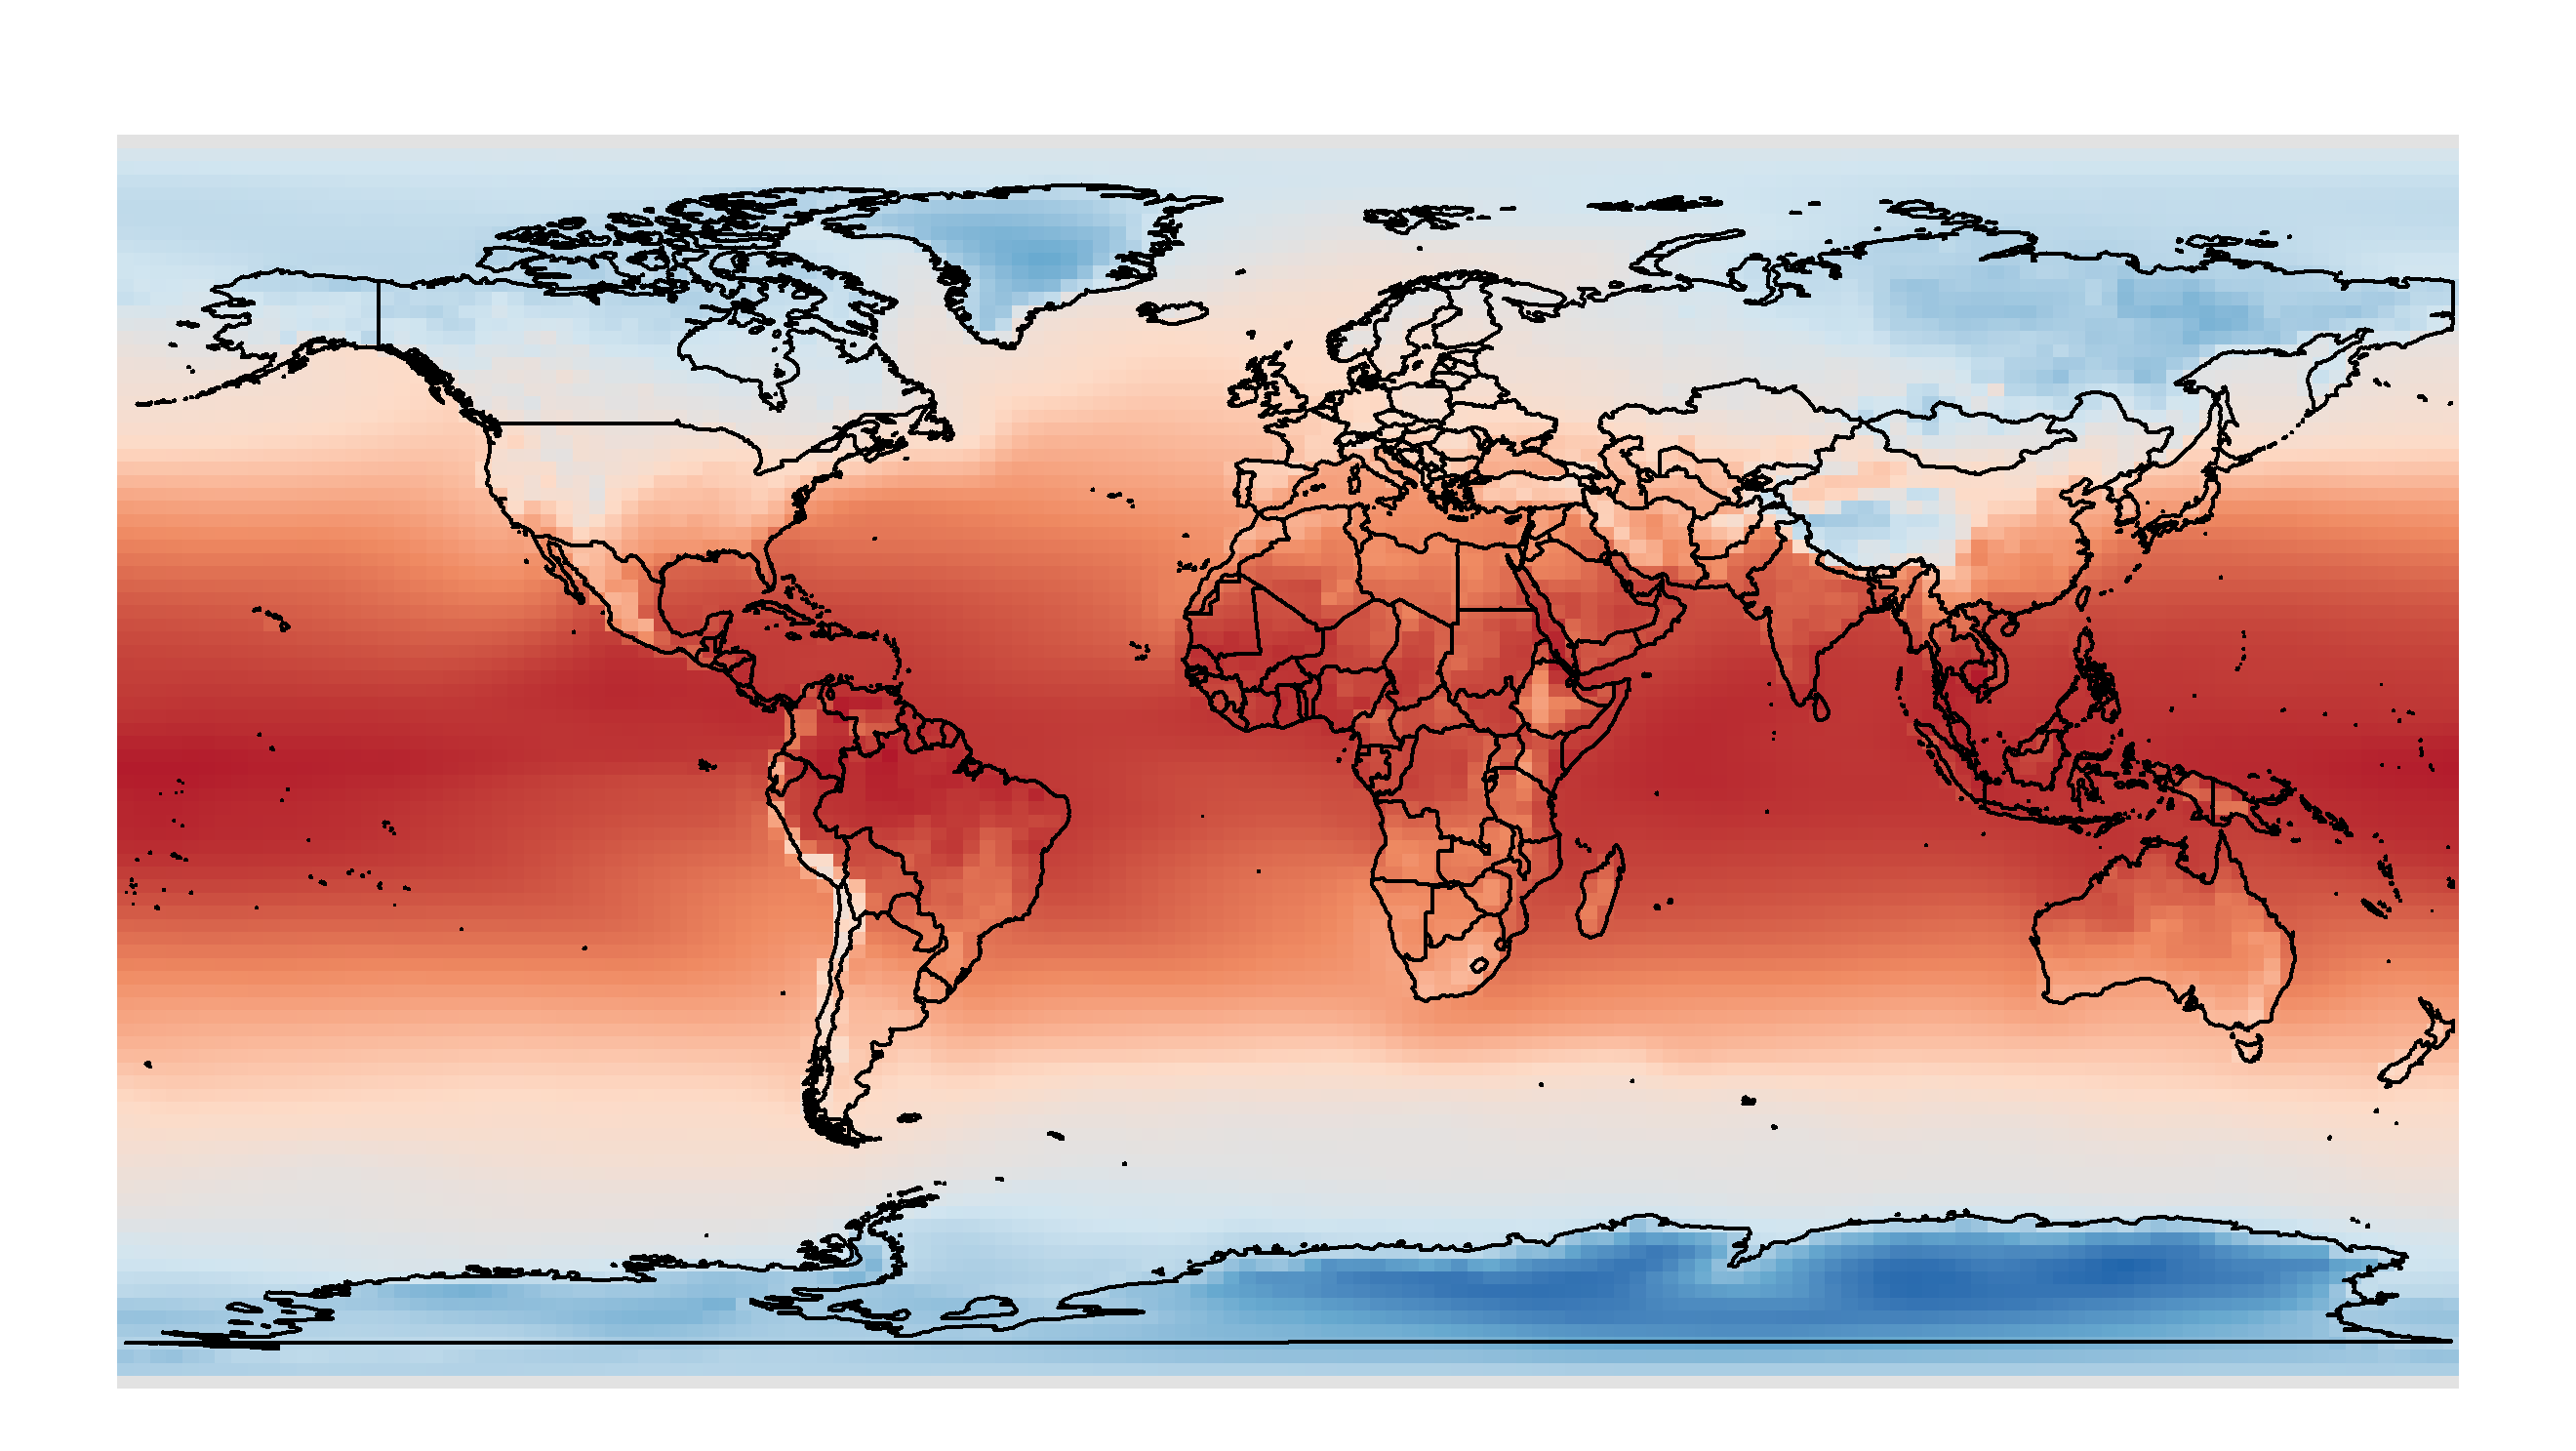
\includegraphics[width=0.45\textwidth]{misc/background.png}
  }
  \subfloat{%
    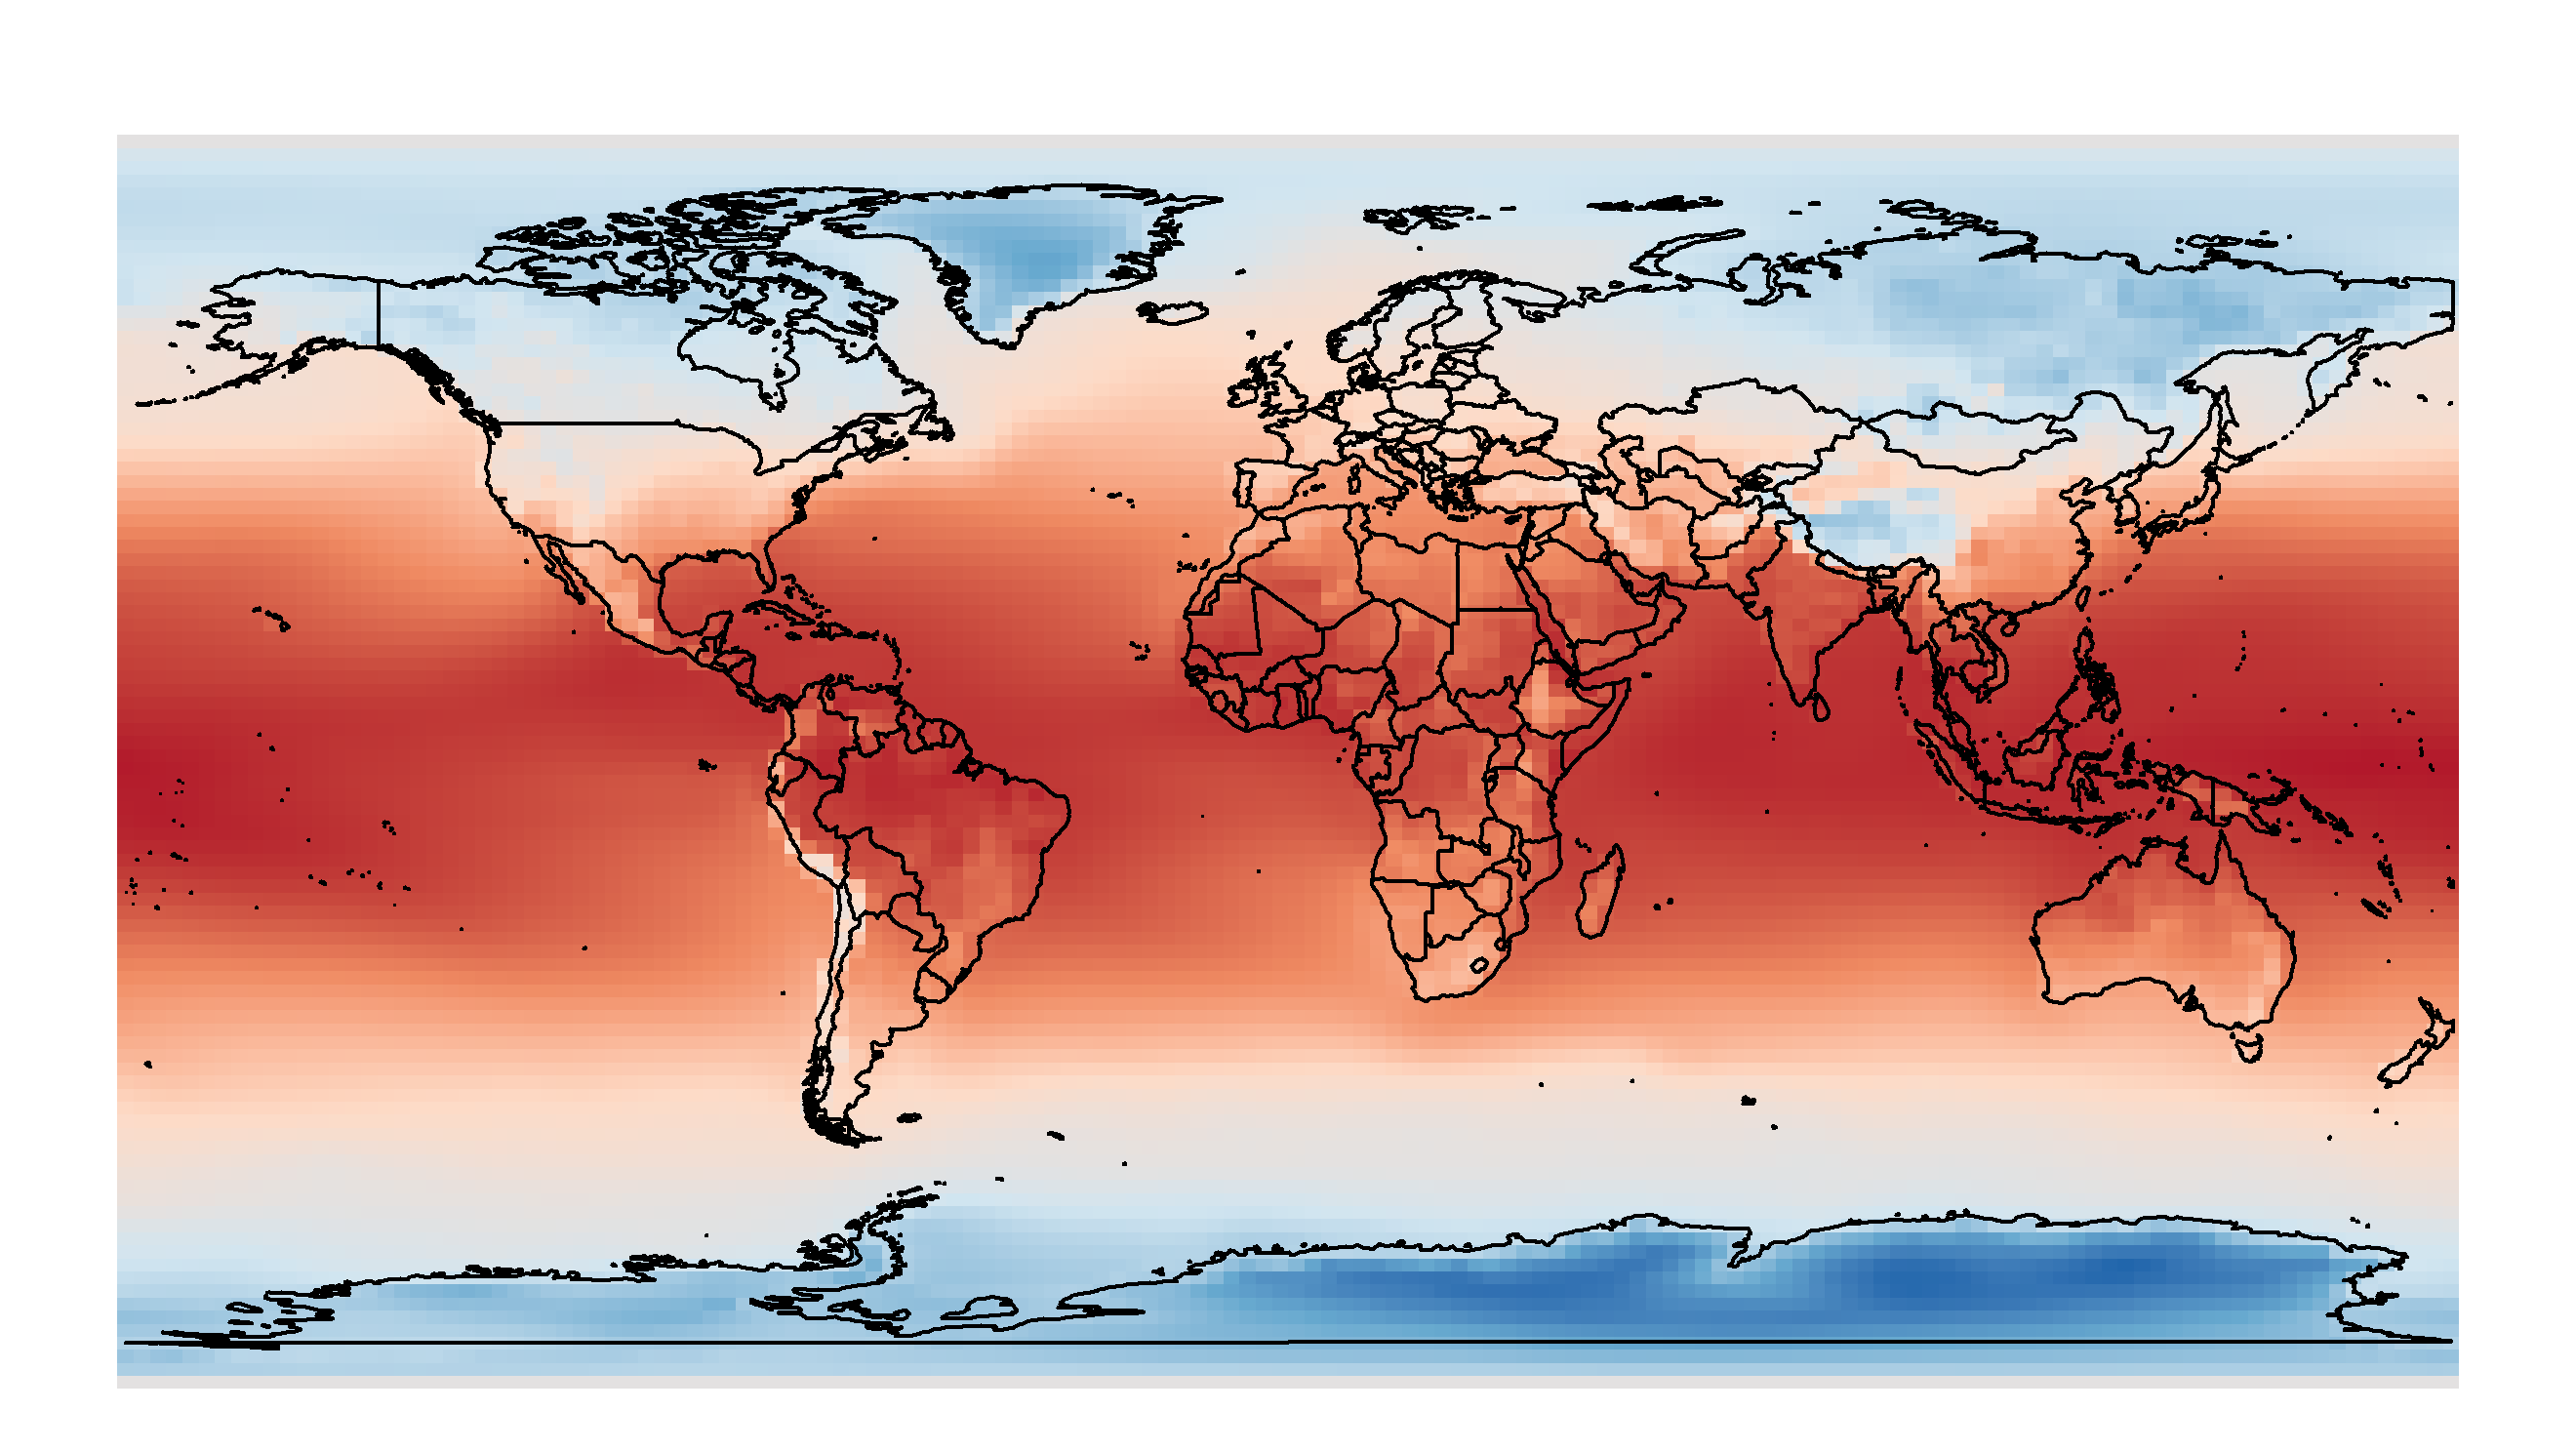
\includegraphics[width=0.45\textwidth]{misc/analysis.png}
  }
  \caption{An example of a background field from the CESM ensemble (left) and an assimilated field in the analysis ensemble (right) in 860 CE.}
  \label{fig:example}
\end{figure}

\subsection{Previous work in random fields comparison} \label{previous}
Comparing two spatial processes has been addressed in both geostatistics and functional data analysis literatures. The general strategy for all those methods is to reduce the dimension of the random process either by a low rank decomposition or  by parameterization, and then develop the test for comparison in the reduced dimension.


From the geostatistical point of view,  wavelet decomposition has been used to reduce the stochastic process to a finite number of  wavelet coefficients and thus the comparison between two processes is transformed to evaluating the difference between two sets of wavelet coefficients \citep{briggs, shen, pavlicova}. 
 \citet{snell} and \citet{wang} extended the method of comparing two time series by evaluating their average loss differentials over the forecast error to assessing the loss function of spatial interpolations. Later \citet{hering} developed a test that can handle more arbitrary and user specified loss functions. Parametric methods have been mainly focusing on testing equality of the first and second moments. Motivated by \citet{lund} that compared two time series, \citet{li1} proposed a parametric method of jointly assessing the first two moments between two random fields. 
 
Functional data analysis approaches assume the spatial random fields to be noisy realizations of an underlying continuous function observed on a finite grid. Traditional dimension reduction methods for functional data such as functional principal component analysis are usually employed in the method development for comparing two random fields. To date, most functional approaches have focused on testing equality of the mean functions arising from two functional data sets \citep{ramsay, zhang2, horvath, staicu2}, although lately the second order structure of functional data also received its due attention \citep{zhang1}. \citet{li2} extended \citet{zhang1} to evaluate the joint difference in mean and covariance structure as well as in trend surface between two spatiotemporal random fields. A nice feature of functional data analysis approaches as opposed to geostatistical methods is that usually assumptions about distribution and model specification are relaxed though at the price of requiring replicates with functional data.  
 
All the above procedures are however inadequate to our problem, because the proxies can affect both mean and covariance structure and higher order structure of the climate field \bl{Is DA able to alter the higher order structure of climate field?}. Furthermore, the rich ensembles from both the background state and the analysis state allow us to examine more information than mean and covariance. Therefore, we aim to compare the distribution of two ensembles to identify the change caused by proxy. To take advantage of ensembles, we will employ a functional data approach that is both distribution and parameter free. Until recently the problem of comparing distribution of functions has remained relatively untouched. \citet{hall} proposed a Cramer-von Mises-like test by constructing an empirical distribution over each of the samples and measuring the $L^2$ distance between the empirical distributions. Later \citet{benko} introduced a permutation test on the leading coefficients of the common functional principal components (FPCs) and  \citet{corain} introduced three omnibus tests for combining pointwise tests on the observations of the functions. Each of these methods depends on a resampling procedure which renders them computationally prohibitive for data assimilation output.\citet{staicu} proposed a method based on marginal FPCs that does not require resampling. Their test compares the distributions of the marginal FPCs using the two sample Anderson-Darling test and a Bonferroni correction. We initially tried a method similar to theirs but found that the principal components in our data had nearly degenerate distributions and thus failed for being used as a valid test. We conjecture that this could be because the impact of proxies is only limited to local scale and therefore it is difficult for the dominant eigenfunctions to register.

The test we propose is based on the functional data analysis paradigm, but is conceptually different from previous efforts. We will use the concept of data depth to construct a nonparametric statistic for assessing the equality of distributions of two functional data sets. This manner of testing has been explored by \citet{quality} who introduced the Quality Index (QI) for comparing two multivariate distributions. The Quality index essentially measured the mean outlyingness of one sample from another using data depth. Their asymptotic results were later finalized in \citet{xuming} who proved that the asymptotic distribution of the two sample QI was Gaussian. We will extend their ideas to the functional setting and propose a modification that makes our statistic invariant to the reference distribution. The use of depth, and particularly integrated Tukey depth, ensures our test to be computationally efficient, distribution free, and invariant to location, scale, warping, and other nuisance properties that could influence the testing \citep{nagy}.


The rest of the paper will proceed as follows. Section \ref{sec:solution} formulate the problem of evaluating proxy influence into a statistic question and proposes a new test statistic for assessing the exchangeability of two sets of functions. Section \ref{sims} shows simulation results to validate the asymptotic behavior of our new test statistic  and evaluate the size and power of our proposed test. Finally in Section \ref{app} we apply it to the data assimilation model at both the regional and global level and answer the questions laid on in the introduction. Section \ref{discussion} is a small discussion on the results and some directions for future work.


% \section{Reconstruction Data}
\section{Statistical Solution} \label{sec:solution}
\subsection{Formulation of evaluating proxy influence} \label{sec:eval} 

Suppose $X$ and $Y_t$ represent the ensemble in the background state and the ensemble in the analysis state at time $t$ in our DA reconstruction, respectively.  Under our assimilation design, the proxies at time $t$ are the only contributor to the differences between the two sets of ensembles. Our goal then is to define and quantify the differences between $X$ and $Y_t$ at each year in order to quantify the proxy influence.

How much impact that proxies may have on analysis states depend on many factors including the proxy type (e.g., tree ring, ice core, coral), where proxies were collected, and the interval over which the proxies were observed \citep{steiger2018PHYDA}. As shown in Fig. \ref{fig:example}, the effects from proxies may be subtle and hard to visually detect because they may be thinly diffused over a non-contiguous area due to spatial correlations and teleconnections.
It seems unlikely that the totality of their effects would be completely described by changes in the first two moments of the climate field. A more comprehensive approach would instead be to test for changes in the distributions of $X$ and $Y_t$. We thus formulate our problem into the following sequence of hypotheses (\bl{sounds multiple testing is involved}): 
\begin{align}\label{eq:test1}
    H_0: X \stackrel{D}{=} Y_t; \ \ H_A: X \stackrel{D}{\neq} Y_t,
\end{align}
where $\stackrel{D}{=}$ means equality in distribution.
In addition to the outcome of these hypothesis tests at each time $t$, we are also equally interested in the pattern to those outcomes at $t$ increases. Since proxies are progressively added into the background states, we may expect that differences between the two distributions increase over time. 
%In section \ref{global} we affirmatively answer this and find a steadily increasing separation between the background and analysis ensembles. In section \ref{regional} we further partition the fields into oceanic and continental regions and observe a similar effect at the regional level.


% \subsection{Data Depth -- MERGE INTO ABOVE OR DELETE}
% Data depth is a statistical concept for quantifying the ``centralness'' or ``outlyingness'' of observations with respect to a population or finite sample. Many different depth functions have been proposed 

% The depth function, which quantifies centralness, is typically based on a distance function or empirical probability measure and must meet several criteria to be considered a proper depth. See \citet{zuo} for multivariate depth and \citet{mosler} for functional depth. Meeting these criteria ensures that a given depth function is measuring centralness in a logical and consistent way. 

% Today there are a wide variety of depth functions for both multivariate and functional data. Multivariate depth has a longer history starting from the Half Space depth \citep{tukey} and then Simplicial depth \citep{simplicial}. Later many other depth functions were developed including the projection depth \citep{proj}, geometric quantiles \citep{geoquant}, and spatial depth \citep{spatial}. Each of these has different strengths and weaknesses with none being said to dominate the others \citep{zuo}. In \citet{muniz} the first depth function for functional data, called integrated depth (ID), was proposed. The integrated depth repeatedly projects the functions into $\mathbbm{R}$ and averages the univariate depths of the projections. Typically the projections are taken to be the values of the functions at each point along their collective domain. Different integrated depths are distinguished by the choice of univariate depth. Since then other types of functional depth have been developed such as the Integrated Band depth \citep{banddepth} and the Extremal depth \citep{naveen}.

% Depth has been successfully used in a variety of applications including outlier detection \citep{outliers}, classification \citep{class}, and robust location estimation. 

% More relevantly though it can be used  hypothesis testing \citep{quality}. \citet{quality} proposes a statistic called the Quality Index that used depth to measure the outlyingness of a sample from some reference distribution. The two sample Quality Index was to the best of our knowledge the first and only test statistic for the equality of two distributions using depth. This test enjoyed asymptotic normality, but it wasn't until \citet{qasymptotic} that the limiting distribution and power functions were derived in general.


%\subsection{Methods} \label{methods}
Under the functional data analysis regime we assume that the observed data are generated from continuous functions combined with additive noise, instead of from spatially correlated stochastic processes. In this framework, each ensemble member represents a single observation over a spatial domain where $144 \times 96$ grid points are embedded. This distinction allows us to consider each ensemble member as an \textit{i.i.d} realization of a stochastic process on a functional space. %This level of abstraction makes the problem analogous to that of comparing the empirical distribution of two sets of \textit{i.i.d} points.

%\subsection{Statistical Framework} \label{framework}
Suppose we observe two sets of functional data, $X = \{(s, X_i(s))_{s \in D}\}_{i = 1}^n$ and $Y = \{(s, Y_j(s)_{s \in D})\}_{j = 1}^m$, where $D$ is a compact subspace of $\mathbbm{R}^p$. For simplicity, $D$ is set to be $[0, 1]^p$ and we assume each functional data is observed on the same set of grid points in $[0, 1]^p$.  Furthermore, we assume each function $X_i$ and $Y_j$ is a univariate continuous function on the domain $[0, 1]^p$, i.e. 
$X_i : [0, 1]^p \mapsto \mathbbm{R} \hbox{ for } i \in 1,\ldots,n$; $Y_j : [0, 1]^p \mapsto \mathbbm{R} \hbox{ for } j \in 1,\ldots,m.$
In other words, each $X_i$ (or $Y_j$) is an element of the class of univariate continuous functions on $[0, 1]^p$, denoted by $C[0, 1]^p$. We therefore consider each functional data $X_i$ (or $Y_j$) as being a random sample from a process in $C[0, 1]^p$. For our data, we have $p = 2$ and $X_i(s)$ and $Y_j(s)$ respectively represent the $i$th background state and the $j$th analysis state at location $s$.

Let $P$ and $Q$ be two absolutely continuous distributions in $C[0,1]^2$ and suppose each $X_i \sim P$ and $Y_j \sim Q$. As mentioned in section \ref{sec:eval}, we are interested in testing if the functional data in $X$ and in $Y$ follow the same distribution, then (\ref{eq:test1}) is equivalent to the hypothesis
\begin{align}\label{eq:test2}
    H_0: P = Q;  \ \ H_A: P \neq Q.
\end{align}
We will use data depth to construct a two sample Kolmogorov-Smirnov type test. Other distribution free tests such as Anderson-Darling or Cramer-Von Mises test could equally have been applied. We chose Kolmogorov-Smirnov for its convenient asymptotic form and its ubiquity in testing distributions.

% Let $X = \{X_1,...,X_n\}$ and $Y = \{Y_1,...,Y_m\}$ be two collections of spatial random fields, such as the background and analysis ensembles at some time $t$ in a reconstruction. Each field $X_i$ or $Y_j$ might then represent some climate variable like surface temperature or the precipitation index over the Earth's surface during a particular year. Our goal is to define and quantify the differences between $X$ and $Y$ and asses the significance of those differences. Most comprehensively we would compare the distribution of $X$ with the distribution of $Y$. We do not want to impose any parametric form on the random fields, so that any differences in the distributions are learned directly from the data. We adopt the functional data analysis approach and represent each random field $X_i$ and $Y_j$ as a continuous random surface on the domain $[0, 1]^2$.\, i.e. 
% \begin{align*}
%     X_i &: [0, 1]^2 \mapsto \mathbbm{R} \quad \forall i \in 1,..,n \\
%     Y_j &: [0, 1]^2 \mapsto \mathbbm{R} \quad \forall j \in 1,..,m.
% \end{align*}
% In other words we say that each $X_i$ and $Y_j$ is an element of the class of continuous functions on $[0, 1]^2$, denoted $C[0, 1]^2$. Therefore, we will consider absolutely continuous distributions on the function space $C[0, 1]^2$, instead of joint distributions over the points in each field.

% Let $P$ and $Q$ be two unknown distributions on $C[0,1]^2$ and suppose $X \sim P$ and $Y \sim Q$. A functional representation allows us to use the aforementioned functional data depth to indirectly characterize differences between the processes $P$ and $Q$. This has most prominently been used in the multivariate setting as justification for depth-depth or DD-plots \citep{ddplots} and as the basis for the Quality Index \citep{quality}. They demonstrate how differences in the moments of $P$ and $Q$ manifest themselves as differences in the depths computed with respect to $P$ and $Q$. We lift this idea to function spaces by swapping in a functional depth and using it to construct a hypothesis test for $P = Q$.

\subsection{Data depth and integrated Tukey depth} \label{depth}
Data depth is a statistical concept for quantifying the ``centralness'' or ``depth'' of the observed data points with respect to a reference distribution. The closer an observation is located to the median of the distribution the more central it is and hence the higher its depth value. Since the reference distribution is typically unknown the depth has to be estimated via depth functions. Many depth functions have been developed for functional data including the integrated band depth \citep{banddepth}, extremal depth \citep{naveen}, and various integrated depths \citep{muniz}. Each of these depth functions has its own strengths and weaknesses but none dominates the others in all aspects, see \citet{cuevas} and \citet{nagy} for a review. We choose the integrated depth as the basis of our test for its simplicity, computational tractability, and highly desirable theoretical properties. 

Integrated depths are a well studied class of functional data depth measures that are first introduced by \citet{muniz} and then studied extensively by \citet{cuevas} and \citet{nagy}. Integrated depths are defined in two stages. First, a univariate depth function is defined over a collection of one dimensional ``projections" of the data which often refers to the observed values of the functions at each location $s \in D$. The univariate depth is then integrated over these projections to yield the integrated depth. Among all the univariate depths the Tukey and the simplicial depth are perhaps the two most popular ones. They are closely related and both their integrated versions come with strong theoretical guarantees. We opted to use the Tukey depth but the simplicial depth would have been equally effective since the orderings they induce are nearly identical.

The integrated Tukey depth is defined as follows. Let $u$ be an element of $\mathbbm{R}$ and let $F$ be an absolutely continuous distribution on $\mathbbm{R}$. The univariate Tukey depth of $u$ with respect to $F$ is 
\[
D_T(u, F) = \min \{F(u), (1 - F(u-))\}.
\]
To enforce the depth function $D(u, F)$ within the range of $[0, 1]$, we scale $D_T(u, F)$ by 2 and define the scaled depth as
\[
D(u, F) = 2D_T(u, F) = 1 - |1 - 2F(u)|
\]
for a continuous $F$. We can further allow $F$, and consequently $D(\cdot, F)$, to depend on the location $t$. Let $X \in  C[0, 1]^p$, the univariate Tukey depth of $X$ at $t \in [0, 1]$ thus immediately follows as 
\[
D(X(t), F_t) = 1 - |1 - 2F_t(X(t))|,
\]
where $F_t$ is the distribution of $X(t)$. We then define the integrated Tukey depth of $X$, with respect to $P$ in (\ref{eq:test2}), as
\[
D(X, P) = \int_0^1D(X(t), F_t)dt.
\]

To ensure that this depth function is proper we refer to the desirable criteria proposed by \citet{zuo} and later by \citet{mosler}. In \citet{nagy} it was shown that the integrated Tukey depth satisfies translation invariance, function scale invariance, measure-preserving rearrangement invariance, maximality at the center, continuity, and quasi-concavity of the induced level sets. They also demonstrated strong universal consistency and weak uniform consistency of the sample depths. These properties broadly assure us that as a center-out ordering the integrated depth is well behaved.

\subsection{Test statistic} \label{test}
Based on the data depth we propose a test statistic $K$ for our hypothesis (\ref{eq:test2}). Basically, $K$ measures the outlyingness of either $P$ over $Q$ or $Q$ over $P$, give that  $P$ and $Q$ may not always appear mutually outlying from each other as depth only measures centrality. For example, if one of the distributions is nested inside the other then the nested distribution will not appear outlying.

%As in section 2.1 let $X = \{(s, X_i(s))_{s \in D}\}_{i = 1}^n$ and $Y = \{(s, Y_j(s)_{s \in D})\}_{j = 1}^m$ be two sets of curves and suppose that $X_i \sim P$ and each $Y_j \sim Q$. 
Denote $P_n$ as the empirical estimate of $P$ based on the sample $X$ and $Q_m$ the empirical estimate of $Q$ based on $Y$. We start by considering $P_n$ fixed and measuring the outlyingness of $Q_m$ over $P_n$. This proceeds with first defining the following two empirical measures for any given $X_k \in X$:
\begin{align}
  \widehat{F}_n(X_k) &= \frac{1}{n}\sum_{i=1}^n \mathbbm{1}(D(X_i, P_n) \leq D(X_k, P_n)) \label{eq:Fn}\\
    \widehat{G}_m(X_k) &= \frac{1}{m}\sum_{j=1}^m \mathbbm{1}(D(Y_j, P_n) \leq D(X_k, P_n)) \label{eq:Gn}.
\end{align}
%We repeat this calculation for each $X_k \in X$ to obtain $ \widehat{F}_n(X_k)$ and $\widehat{G}_m(X_k)$ for $k=1,\ldots, n$. 
Essentially, $\widehat{F}_n(X_k)$ is a rescaling of the depth of $X_k$ such that $\widehat{F}_n(X_k)=1/n$ if $D(X_k, P_n)$ is the smallest,  $2/n$ if the depth is the second smallest, and so until it reaches 1 when the depth becomes the largest. It acts as the empirical cumulative distribution function of the depths of $X_k$ and thus naturally follows \bl{approximate?} a uniform distribution.  
The second quantity $\widehat{G}_m(X_k)$ can be considered as a transformation of the depths of $Y$ with respect to the depths of $X$.
Under $H_0$ in (\ref{eq:test2}), $\widehat{G}_m$ should be approximately uniform so a deviation of $\widehat{G}_m$ from the uniform distribution indicates an outlyingness of $Q_m$ from $P_n$. The introduction of $ \widehat{F}_n(X_k)$ and $\widehat{G}_m(X_k)$ allows us to reduce the problem of comparing two sets of random fields to assessing the difference in distribution between two sets of random variables, $\widehat{F}_n(X_k)$ and $\widehat{G}_m(X_k)$ for $k=1,\ldots, n$. The latter can naturally be quantified using the Kolmogorov distance over the set $X$ \bl{Is below correct? not sure $X_k$ is placed correctly},
\begin{equation}\label{eq:KPn}
K_{P_n}(X, Y) = \max_{X_k \in X}|\widehat{F}_n(X_k) - \widehat{G}_m(X_k)|.
\end{equation}

To measure the outlyingness of $P_n$ over $Q_m$, we now fix $Q_m$ rather than $P_n$. Following the same scheme, we define the two empirical measures for any given $Y_k \in Y$ as
\begin{align*}
    \widetilde{F}_n(Y_k) &= \frac{1}{n}\sum_{i=1}^n \mathbbm{1}(D(X_i, Q_m) \leq D(Y_k, Q_m)) \\
    \widetilde{G}_m(Y_k) &= \frac{1}{m}\sum_{j=1}^m \mathbbm{1}(D(Y_j, Q_m) \leq D(Y_k, Q_m)).
\end{align*}
 These two quantities exactly mirror $\widehat{F}_n$ and $\widehat{G}_m$ except that now $\widetilde{G}_m$ becomes \bl{approximately?} uniform and $\widetilde{F}_n$ the indicator for the outlyingness of $P_n$ from $Q_m$. We again take Kolmogorov distance, but now over the set $Y$, as the measure of outlyingness,
\[
K_{Q_m} (X, Y) = \max_{Y_k \in Y}|\widetilde{F}_n(Y_k) - \widetilde{G}_m(Y_k)|.
\]

To define the overall test statistic $K$ we take the maximum of the two distances:
\begin{equation}\label{eq:ts}
K(X, Y) = \max\{K_{P_n}(X, Y) \text{, } K_{Q_m}\}.
\end{equation}
The test statistic $K(X, Y)$ attains a level of symmetry by making the test invariant to the reference distribution. It is strictly non-negative and it equals 0 only under $H_0$ in the hypothesis (\ref{eq:test2}). Thus the originally stated hypothesis (\ref{eq:test1}) can be tested by evaluating how significantly $K(X, Y)$ is greater than 0. 
We expect $K(X, Y)$ to detect the difference between $P$ and $Q$ in either mean, scale, or correlation structures, for both situations where there are global shifts in the parameters as well as where parameters change randomly over the domain. The biggest difference between our test statistic $K(X, Y)$ and the Quality Index ($QI$) in \bl{reference} is that our test does not depend on a reference distribution while $QI$ requires to take the distribution of one of the two samples as reference. Our test computes the outlyingness of two samples from each other and aggregates the results into one single test. This is a more efficient use of the two samples and enables to detect a larger range of alternative hypothesis, such as the nesting situation mentioned above. We discuss the critical values of $K(X, Y)$ in the following section. 

 
%To test for significant differences, $K$ need only be compared with the critical values of its asymptotic distribution. Resampling is not necessary but there may be reasons to prefer resampling when the data is very noisy and sample sizes are small, see Figures \ref{crit} and \ref{size2d}.


%%%%% Critical Values
\subsection{Computing critical values} \label{critical}
Deriving the asymptotic distribution of $K(X, Y)$ is nontrivial since $K(X, Y)$ explicitly depends on two non \textit{iid} processes, $D(X_k, P_n)$ and $D(Y_k, Q_m)$. This renders standard results on the Kolmogorov-Smirnov test inapplicable. Nevertheless, we posit without formal proof that $K(X, Y)$ follows the same limiting distribution as the regular Kolmogorov-Smirnov two sample statistic, i.e.
\[
\sqrt{\frac{nm}{n+m}} K(X, Y) \xrightarrow{D} K',
\]
where
\[
P(K' < t) = 1 - 2\sum_{j=1}^{\infty}(-1)^je^{-2j^2t^2}.
\]
Although we are unable to prove this general results, we consider two special cases below and both are shown to conform to the conjecture. Our extensive simulation studies also demonstrate this general convergence. 

%We were able to show a similar result for the one sample version of the test where $P$ is known. We also have a partial result on the two sample test when $n \gg m$ and a simulation study demonstrating that convergence likely holds for the full two sample test. 

We first consider a special case where $P$ is known and we are interested in testing if  $Y_j\sim P$ for $j=1,\ldots, m$. In such case $\widehat{F}_n(X_k)$ in (\ref{eq:Fn}) becomes a random variable $t\sim$uniform$[0, 1]$ and thus $\widehat{G}_m(X_k)$ in (\ref{eq:Gn}) becomes $\widehat{G}_m(t)$. Then $K_{P_n}(X, Y)$ in (\ref{eq:KPn}), which is the test statistics for this special case,  reduces to 
\[
K_{P}(t) = \sup_{t \in [0, 1]}|t - \widehat{G}_m(t)|. 
\]
Since $\widehat{G}_m(t)$ is an empirical distribution of the i.i.d random variables $\{D(Y_1, P), \dots, D(Y_m, P) \}$, $K_{P}(t)$ is exactly the one sample Kolmogorov-Smirnov statistic for testing the uniformity of $\widehat{G}_m(t)$. Therefore,
\[
\sqrt{m} K_P(t) \xrightarrow{D} K.
\]

%We first consider the one sample case where $P$ is known and we want to test if a sample $Y = \{Y_1,...,Y_m\}$ follows $P$. The test $K$ just becomes $K_P$ since there is no second sample to form a second reference test. The set of all $D(x, P)$ becomes $[0, 1]$ and so $K_{P}(P, Q)$ reduces to 

We further consider another special case where $P$ and $Q$ are both unknown but with either $n \gg m$ or $m \gg n$. We can show that $K_{P_n}(X, Y)$ (or $K_{Q_m} (X, T)$) converges to Kolmogorov distribution under $n \gg m$ ($m \gg n$).  
%Combining the two would not be possible since proving the convergence of the combined test would require $n \gg m$ and $m \geq n$ simultaneously. 
We encapsulate this result in the following proposition.
\begin{proposition} \label{asymptotic}
Suppose that $n \gg m$, then under the null hypothesis,
\[
\sqrt{\frac{nm}{n+m}} K_{P_n}(X, Y) \xrightarrow{D} K'
\]
where $K'$ follows the Kolmogorov distribution.
\end{proposition}
The proof is deferred to the Appendix. 
Generalizing the results of special cases to more general setting is challenging. This issue was noted in \citet{quality} where the authors conjectured that their two sample $QI$ asymptotically followed a normal distribution, as its one sample version. Their conjecture was only later proven in \citet{xuming} after substantial theoretical development. The techniques that emerged from the proof in \citet{xuming} relied heavily on $QI$ being an expectation, making them largely inapplicable to our context that involves suprema.
In lieu of an asymptotic distribution we may consider using permutation to find critical values for $K(X, Y)$ \bl{add a reference for purmutation}. Permutation works well for small samples or sparsely observed functions, however it quickly becomes computationally infeasible on large volumes of data, such as our reconstruction data. For this reason, the conjectured Kolmogorov distribution is more appealing in practice. 


%%%%%% SIMULATIONS
\section{Simulation Study} \label{sims}
Simulation studies are conducted to assess the convergence of $K(X, Y)$,  and size and power of the test. 
%Each of these properties were evaluated using both one and two dimensional functional data since our main application considers time series and spatial fields. 
Each of these properties is evaluated using two dimensional functional data since our main application considers ensembles of spatial fields. All functional data in the simulation are generated from Gaussian random processes with an exponential covariance function $C(x, x') = \exp\{-\|x - x'\|/r \}$, where the range parameter $r$ governs how quickly the correlation decays between observations. A small (larger) $r$ indicates a weak (strong) correlation and consequently a rough (smooth) functional data.  We could instead use Mat\'ern covariance function \bl{add reference} to control the smoothness \bl{by looking at the definition of smoothness in http://anson.ucdavis.edu/~mueller/Review151106.pdf and the mean square differentiability in my spatial class notes, it looks Matern may be more appropriate?}
In each simulation we consider the sample $X$ as the baseline and $Y$ as the sample to be varied. 

\subsection{Convergence} \label{sec:conv}
We use simulations to validate the conjectured asymptotic Kolmogorov distribution of our test statistic \ref{eq:ts} under the null hypothesis. The main idea is to evaluate how well the permutation distribution is approximated by the Kolmogorov distribution, even at moderate sample size.  The functional data $X$ and $Y$ are generated with mean $\mu = 0$ and standard deviation $\sigma = 1$ on spatial domain $[0, 20] \times [0, 20]$. Since the integrated Tukey depth is invariant to location and scale, we only vary the range parameter $r$ to be 5, 10, 15, and 20 as well as the number of replicates $n$ to be 25, 50, 100 and 150 in studying the convergence of the asymptotic distribution of the test statistics. 
Unbalancing sample sizes enabled much faster convergence since $K(X, Y)$ would behave more like either of its one sample versions \bl{Is this shown in Figure 2 and 3?}. 
The permutation distribution was constructed by recomputing $K(X, Y)$ on 2000 permutations of the generated $X$ and $Y$ samples. Then we calculate the $L^2$ distance between the permutation distribution and the Kolmogorov distribution. In addition, we also calculate the difference in critical values derived from either the Kolmogorov or the permutation distribution at three common significance levels: 0.01, 0.05 and 0.10. 
We run simulation 100 times for each combination of $r$ and $n$ to obtain the boxplots in Figures \ref{rmse} and \ref{crit}.

\begin{figure}
	\begin{center}
    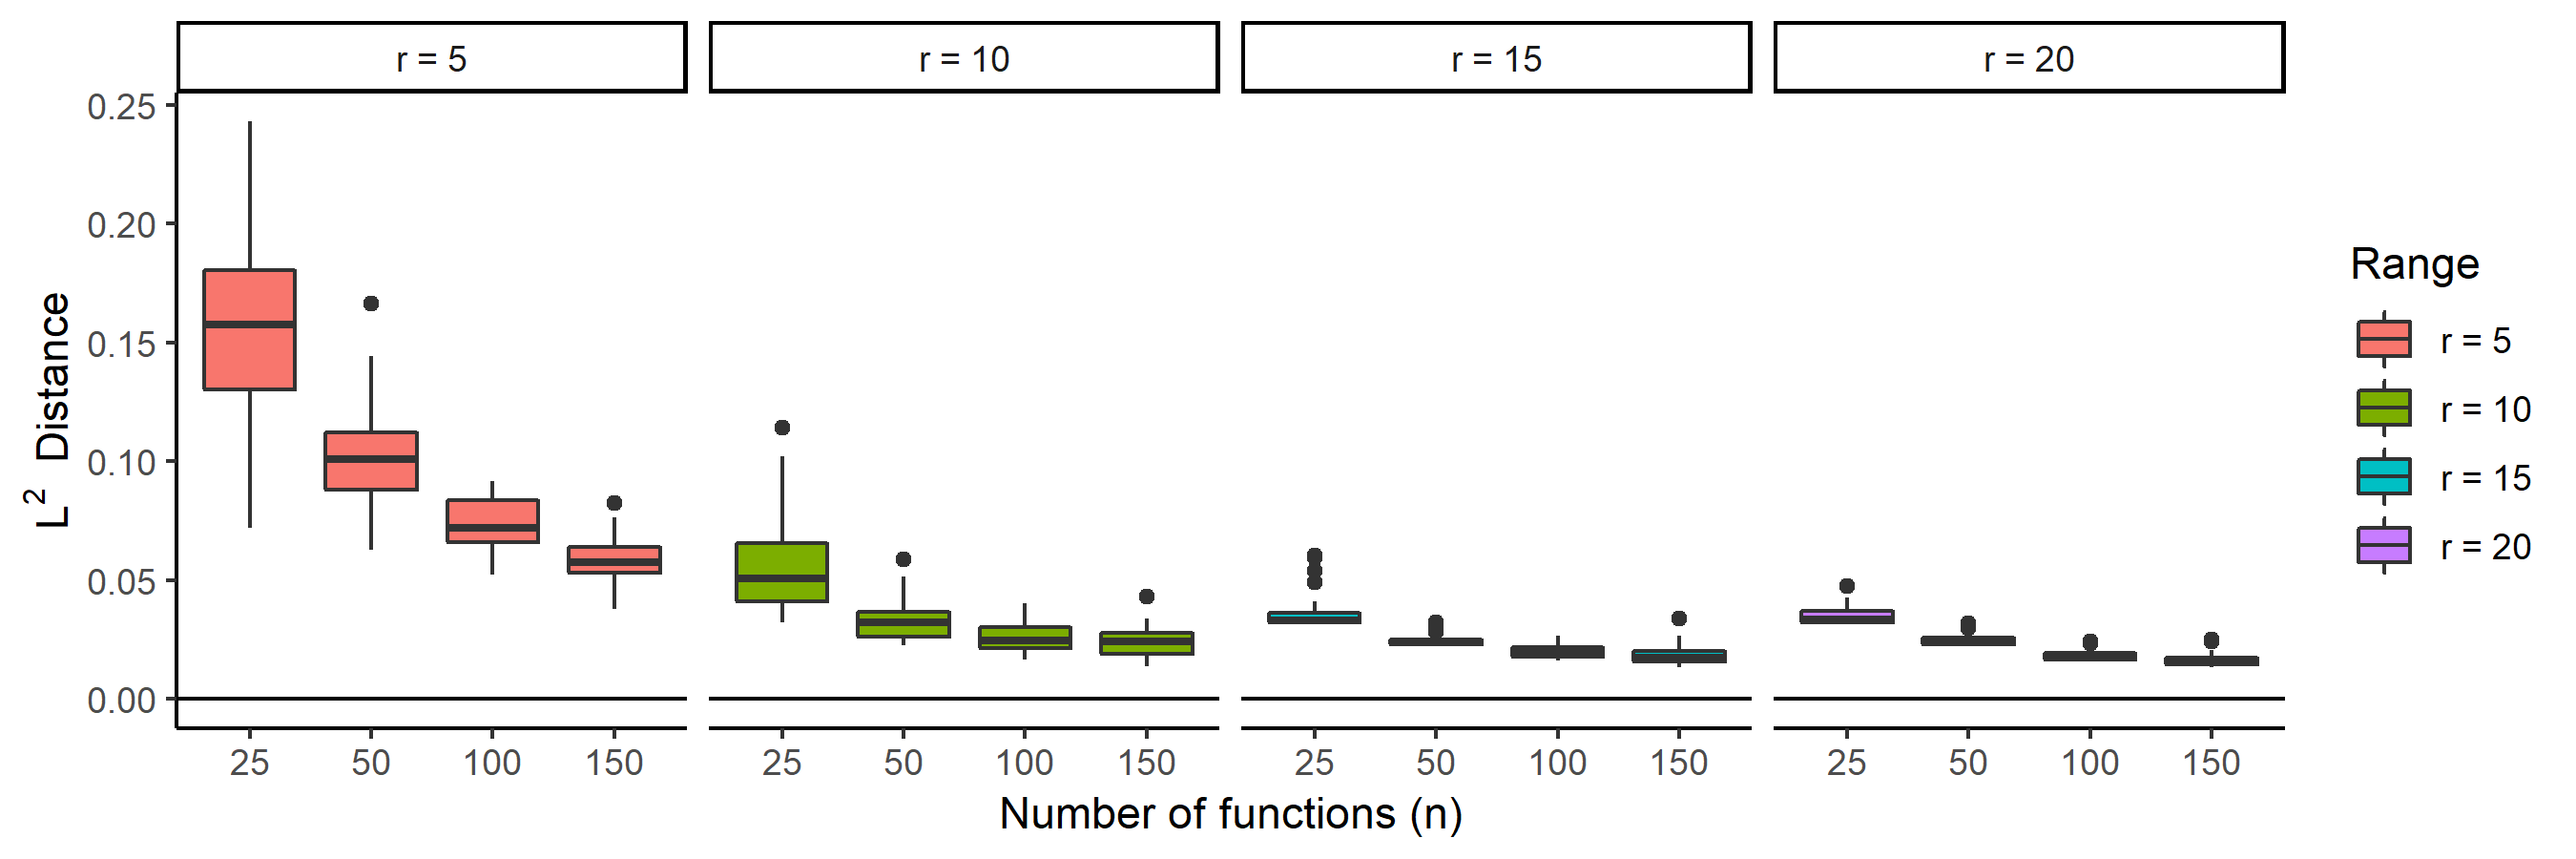
\includegraphics[width=0.80\textwidth,valign=c]{conv/conv1.png}
    \caption{$L^2$ distance between the permutation distribution and the Kolmogorov distribution under 16 different range and sample size settings.}
    \label{rmse}
    \end{center}
\end{figure}

Figure \ref{rmse} demonstrates convergence of the permutation distribution to Kolmogorov in $L^2$. For even small sample sizes such as $n = 25$, the distance between the two distributions is already vanishingly small for smooth data ($r= 10, 15, 20$). The $r \leq 5$ case is typically not an obstacle in practice because functional data would usually be preprocessed with a smoothing step. In all cases the $L^2$ distance decays rapidly with an increasing sample size so even noisy data can be compensated for if the sample size is large enough.

Figure \ref{crit} evaluates the convergence of two sets of critical values at three common significance levels: 0.01, 0.05 and 0.10. This figure aims to answer the question of   how much bias if any in making decisions with the asymptotic Kolmogorov distribution and the permutation, even if the two distributions are not in exact agreement. 
Again, a sufficient amount of smoothness ($r > 5$) is required to have well behaved critical values. If the data is not sufficiently smooth the Kolmogorov distribution tends to have smaller critical values than its corresponding permutation distribution. The size will therefore be slightly inflated by using Kolmogorov and so the permutation distribution should be preferred when computationally feasible. Once a sufficient level of smoothness has been reached, in this case $r \geq 10$, the critical values of the permutation distribution become highly agreeable to the Kolmogorov's. The observed differences are minuscule so any decision reached using the Kolmogorov distribution is likely to be same as if the permutation distribution were used.

\begin{figure}
	\begin{center}
    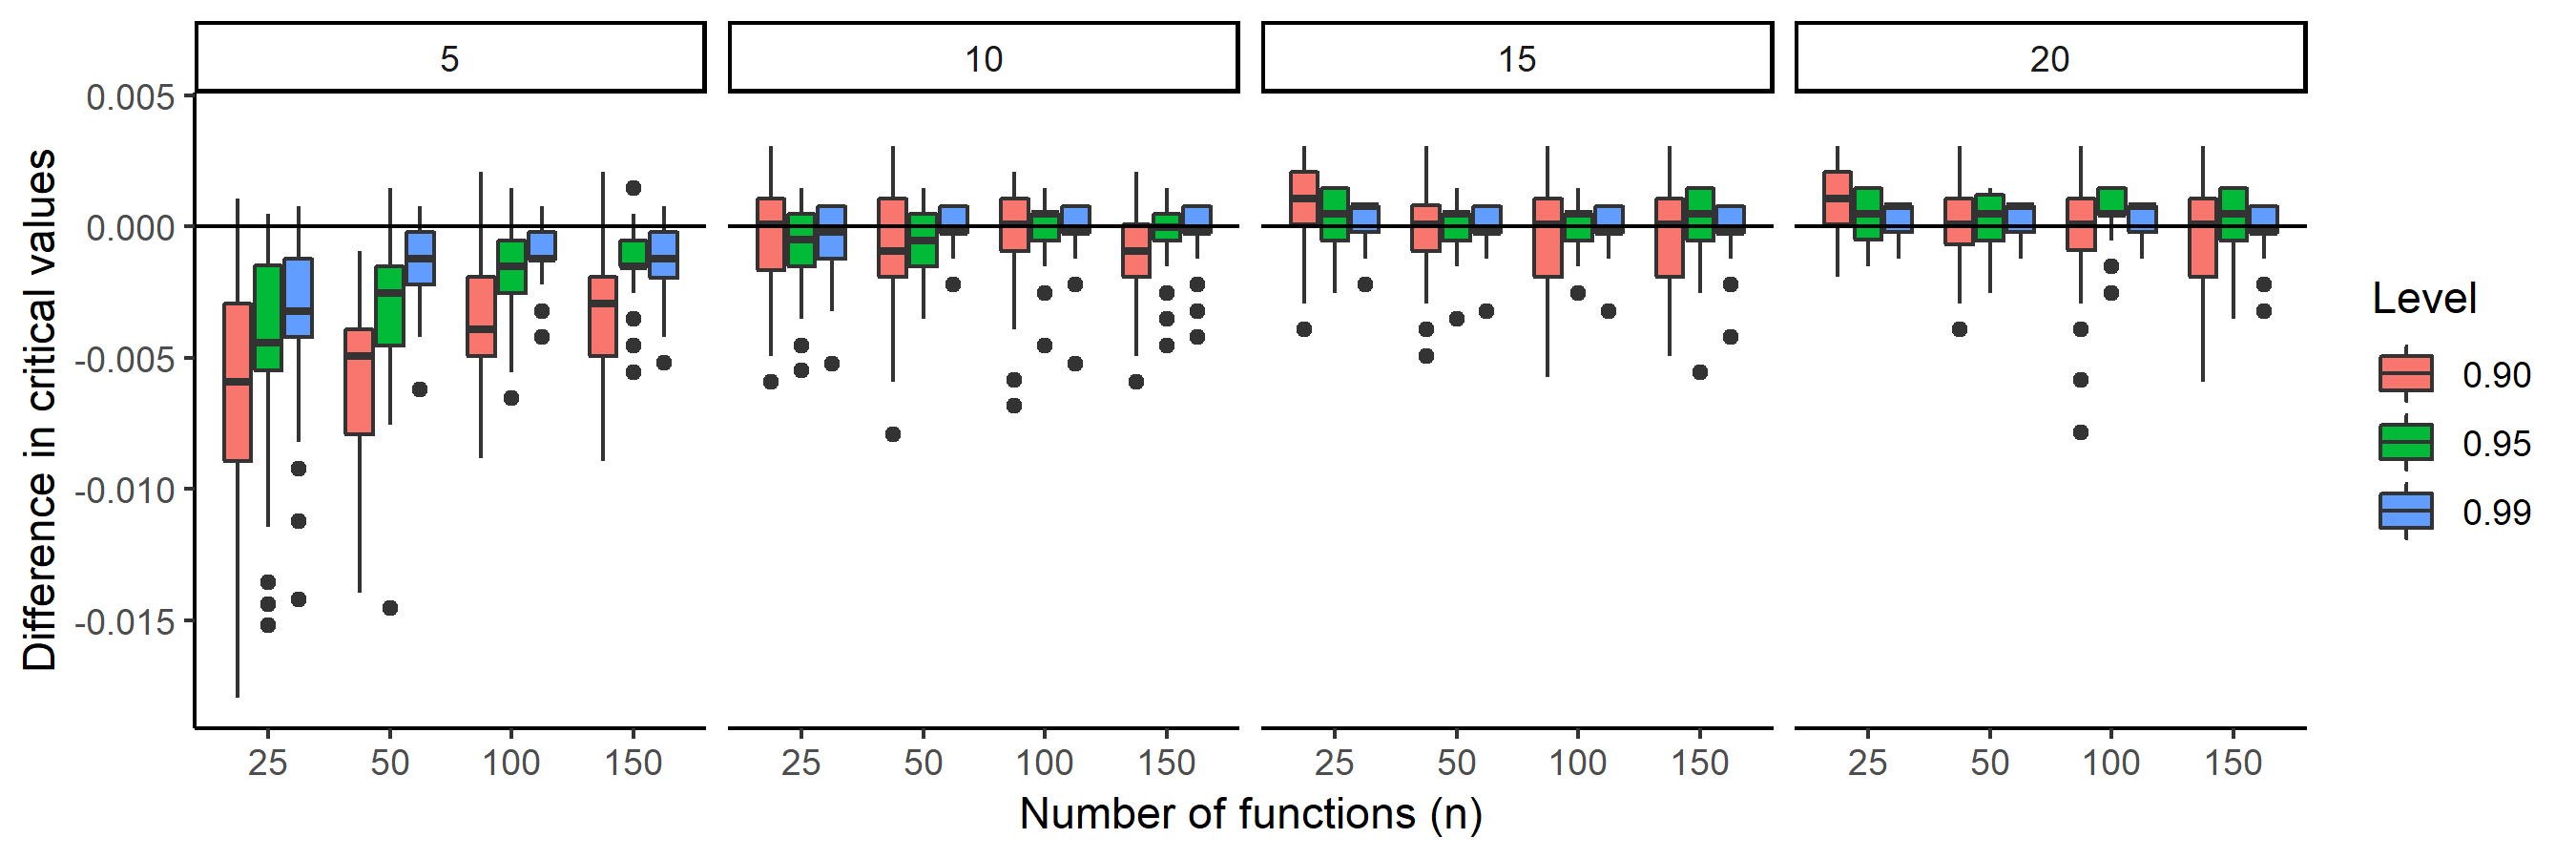
\includegraphics[width=0.80\textwidth,valign=c]{conv/conv2.png}
    \caption{Kolmogorov critical values minus permutation critical values at three common test levels: 0.90, 0.95. 0.99 under 16 different range and sample size settings.}
    \label{crit}
    \end{center}
\end{figure}

\subsection{Size and power} \label{size}
Using the same data generating process as in \ref{sec:conv},  we evaluate the size of our test using critical values from the asymptotic Kolmogorov distribution and also compare our size to the $QI$ test. 
Again only the range $r$ and sample size $n$ will be varied. The size under each combination of $r$ and $n$ was estimated 50 times \bl{How to get size 50 times for each simulation?} using 1000 simulations apiece; the results of which are summarized in Figure \ref{size2d}.  
Our simulations show that for even a small sample such as $n = 50$, our test is able to control the size near the prescribed level if $r > 5$. As in the convergence simulation this smoothness condition is not all that impactful in practice since functions are typically smoothed before analysis. For functional data with $r \geq 10$, the size of our test is controlled very near the nominal level even for small sample sizes. Moreover, the range no longer seems to play a role beyond a threshold between 5 and 10 for the spatial domain $[0, 20] \times [0, 20]$. The $QI$ test appears to inflate the size in all cases compared to our test. 

\begin{figure}
	\begin{center}
    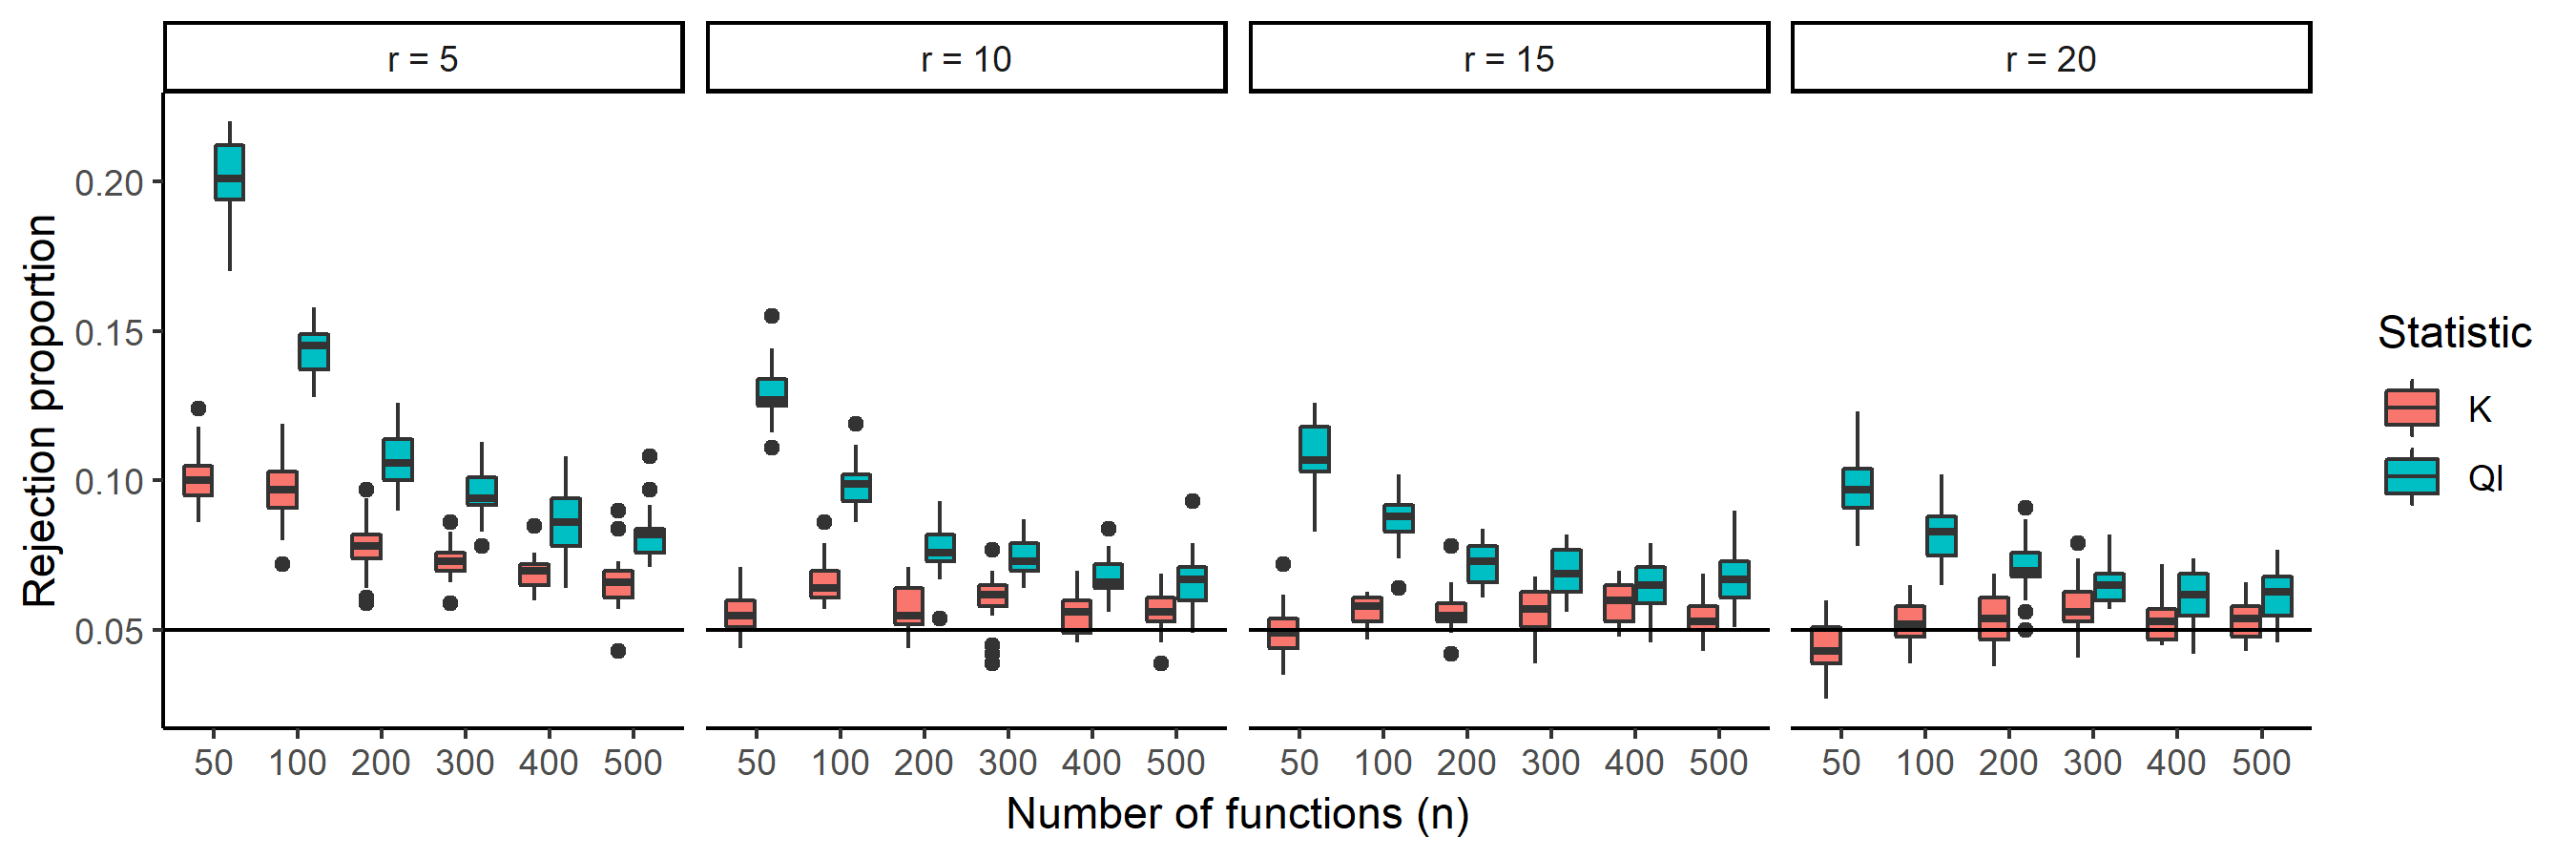
\includegraphics[width=0.8\textwidth,valign=c]{size/size2d2.png}
    \caption{Size for $K$ and $QI$ under 16 different combinations of range and sample size ordered from noisiest (r = 5) to smoothest (r = 20). Black line at 0.05 designates the nominal level of the test.}
    \label{size2d}
    \end{center}
\end{figure}



% We also compared the empirically attained sizes of $K$ and $QI$ on one dimensional functional data, Fig. \ref{size1d}. This time $X$ and $Y$ were sampled from a one dimensional Gaussian process with mean $\mu = 0$, standard deviation $\sigma = 1$, and covariance function $\gamma(x, x') = \exp\{-(x - x')^2/r \}$. Functions were sampled on the domain $[0, 50]$ and were not smoothed or interpolated further. Again only the range $r$ and the sample size $n$ were varied and for each combination of $r$ and $n$ the rejection proportion was estimated 50 times using 1000 simulations each. The results are similar to those obtained under the two dimensional setting and are summarized in figure \ref{size1d}. The proportion of rejections are controlled more closely to the nominal level than the two dimensional functions, since the same value of $r$ implies stronger correlation in 1D data than it would in equivalently sampled 2D data.

% \begin{figure}
% 	\begin{center}
%     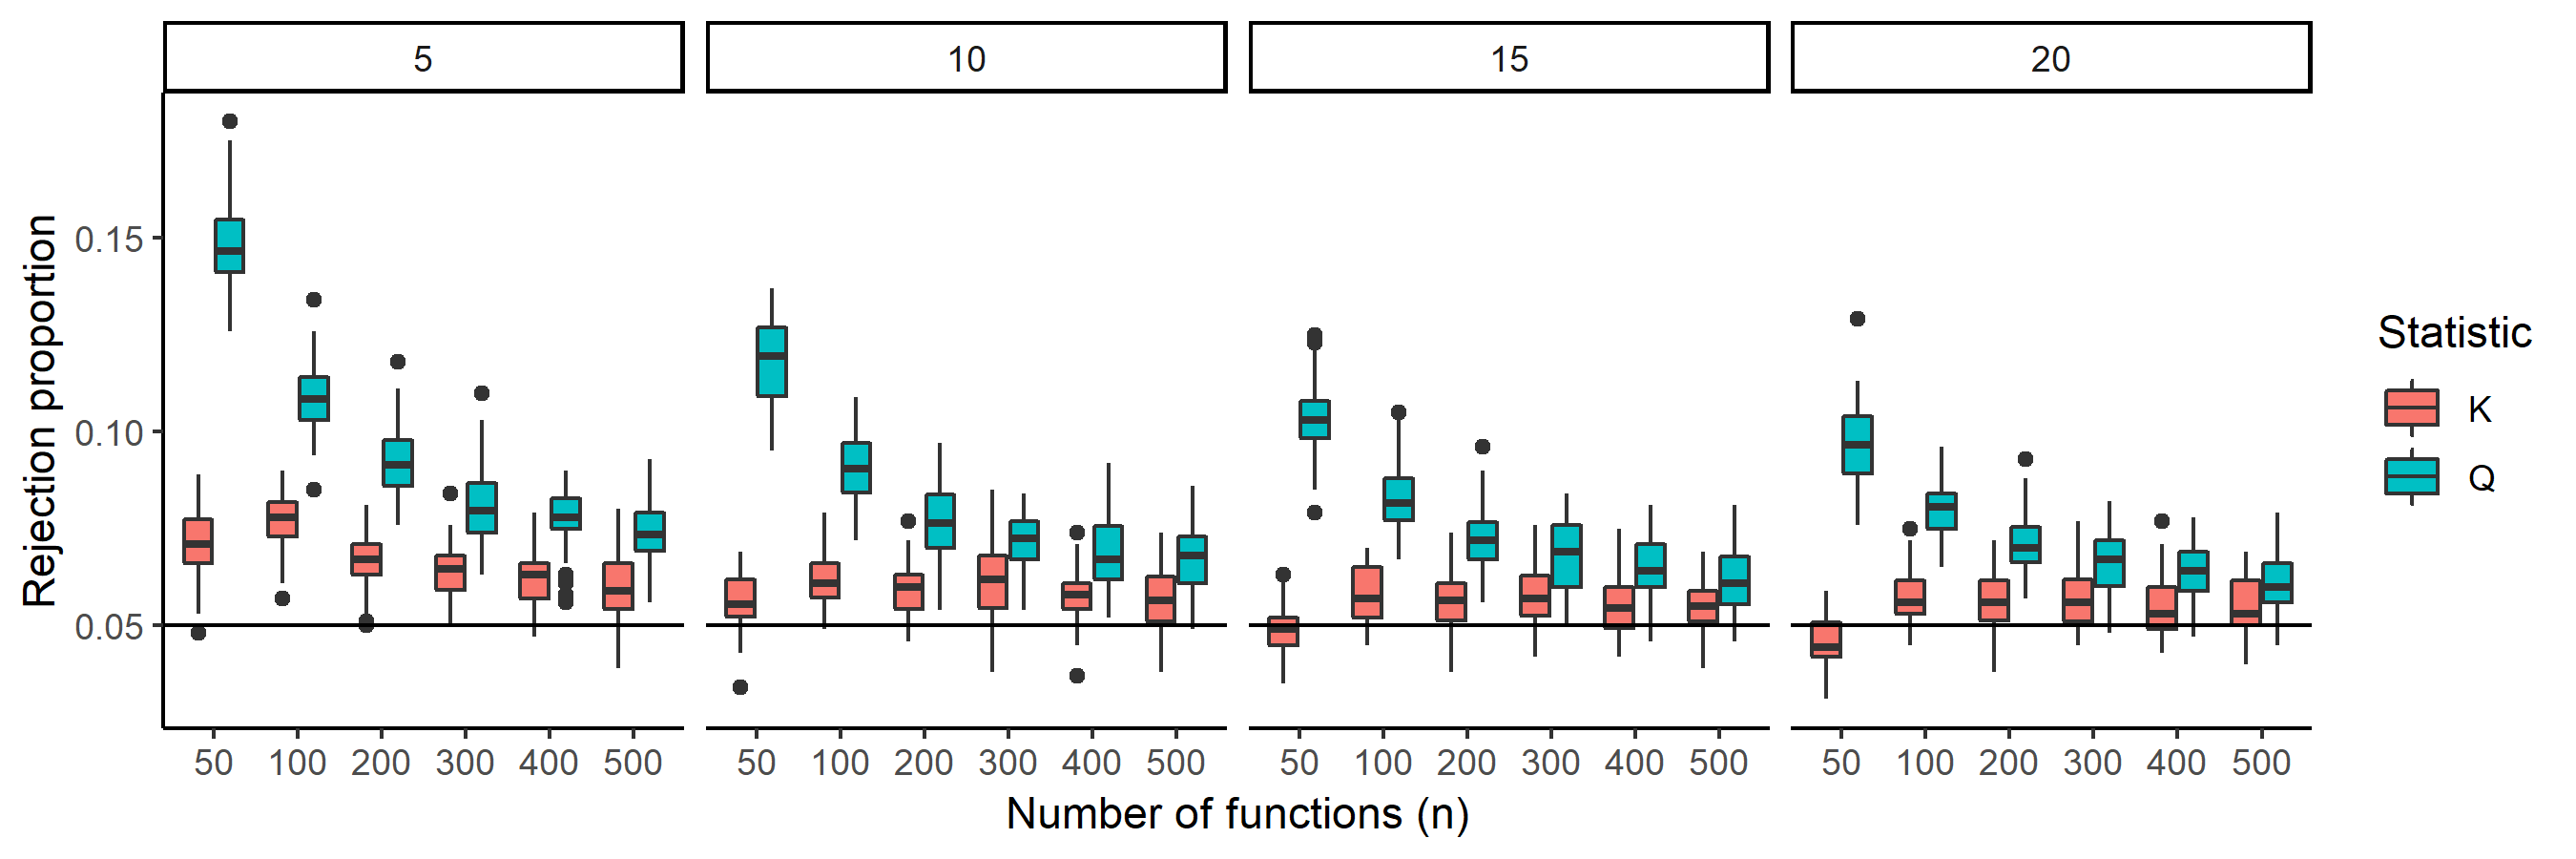
\includegraphics[width=0.8\textwidth,valign=c]{size/size1d2.png}
%   \caption{\textbf{One Dimensional:} Empirical size estimates for $K$ and $QI$ under 16 different range and sample size settings ordered from noisiest (r = 5) to smoothest (r = 20). Black line at 0.05 designates the specified type one error rate.}
%     \label{size1d}
%     \end{center}
% \end{figure}

%Overall these simulations demonstrate that the size of $K$ is well controlled at the nominal level under the Kolmogorov distribution. The most important factor for controlling size was found to be the smoothness of the data; up until some threshold is reached. In the simulations presented here an $r$ value between 5 and 10 was sufficient to control the size of $K$ for data observed on the domain $[0, 20] \times [0, 20]$. This held even when the sample sizes were quite small, i.e. between 50 and 100. If the data were observed on a larger domain, such as the data assimilation output, then a larger degree of smoothness would perhaps be required. 


%\subsection{Power} \label{power}
Then we compare the power of our test and $QI$ test in detecting changes in the three parameters $\mu$, $\sigma$, and $r$ which govern the underlying Gaussian process in our data generation. For power calculation, the sample size was fixed at $n = m = 400$ functions per sample so that $K$ and $QI$ would have comparable type I error rates\bl{why?}. The functions in $X$ are still generated from the Gaussian process with $\mu = 0$ and $\sigma = 1$ while $r$ set to four different values: 5, 10, 15 and 20. This yields four baseline models for $X$ at different smoothness levels. We then generate $Y$ samples corresponding to each baseline model by setting the parameter of interest to different values. In order to examine the power curve we vary the mean of $Y$ from -1 to 1, the standard deviation from 0.5 to 1.5 and the range from 5 to 80. 
We compute the power of our test to detect changes from each of these four baseline models in all three parameters, and then compare to the $QI$ test. Each power is calculated from 500 simulation runs \bl{why the number of simulation runs keeps changing?}  


\begin{figure}
	\begin{center}
    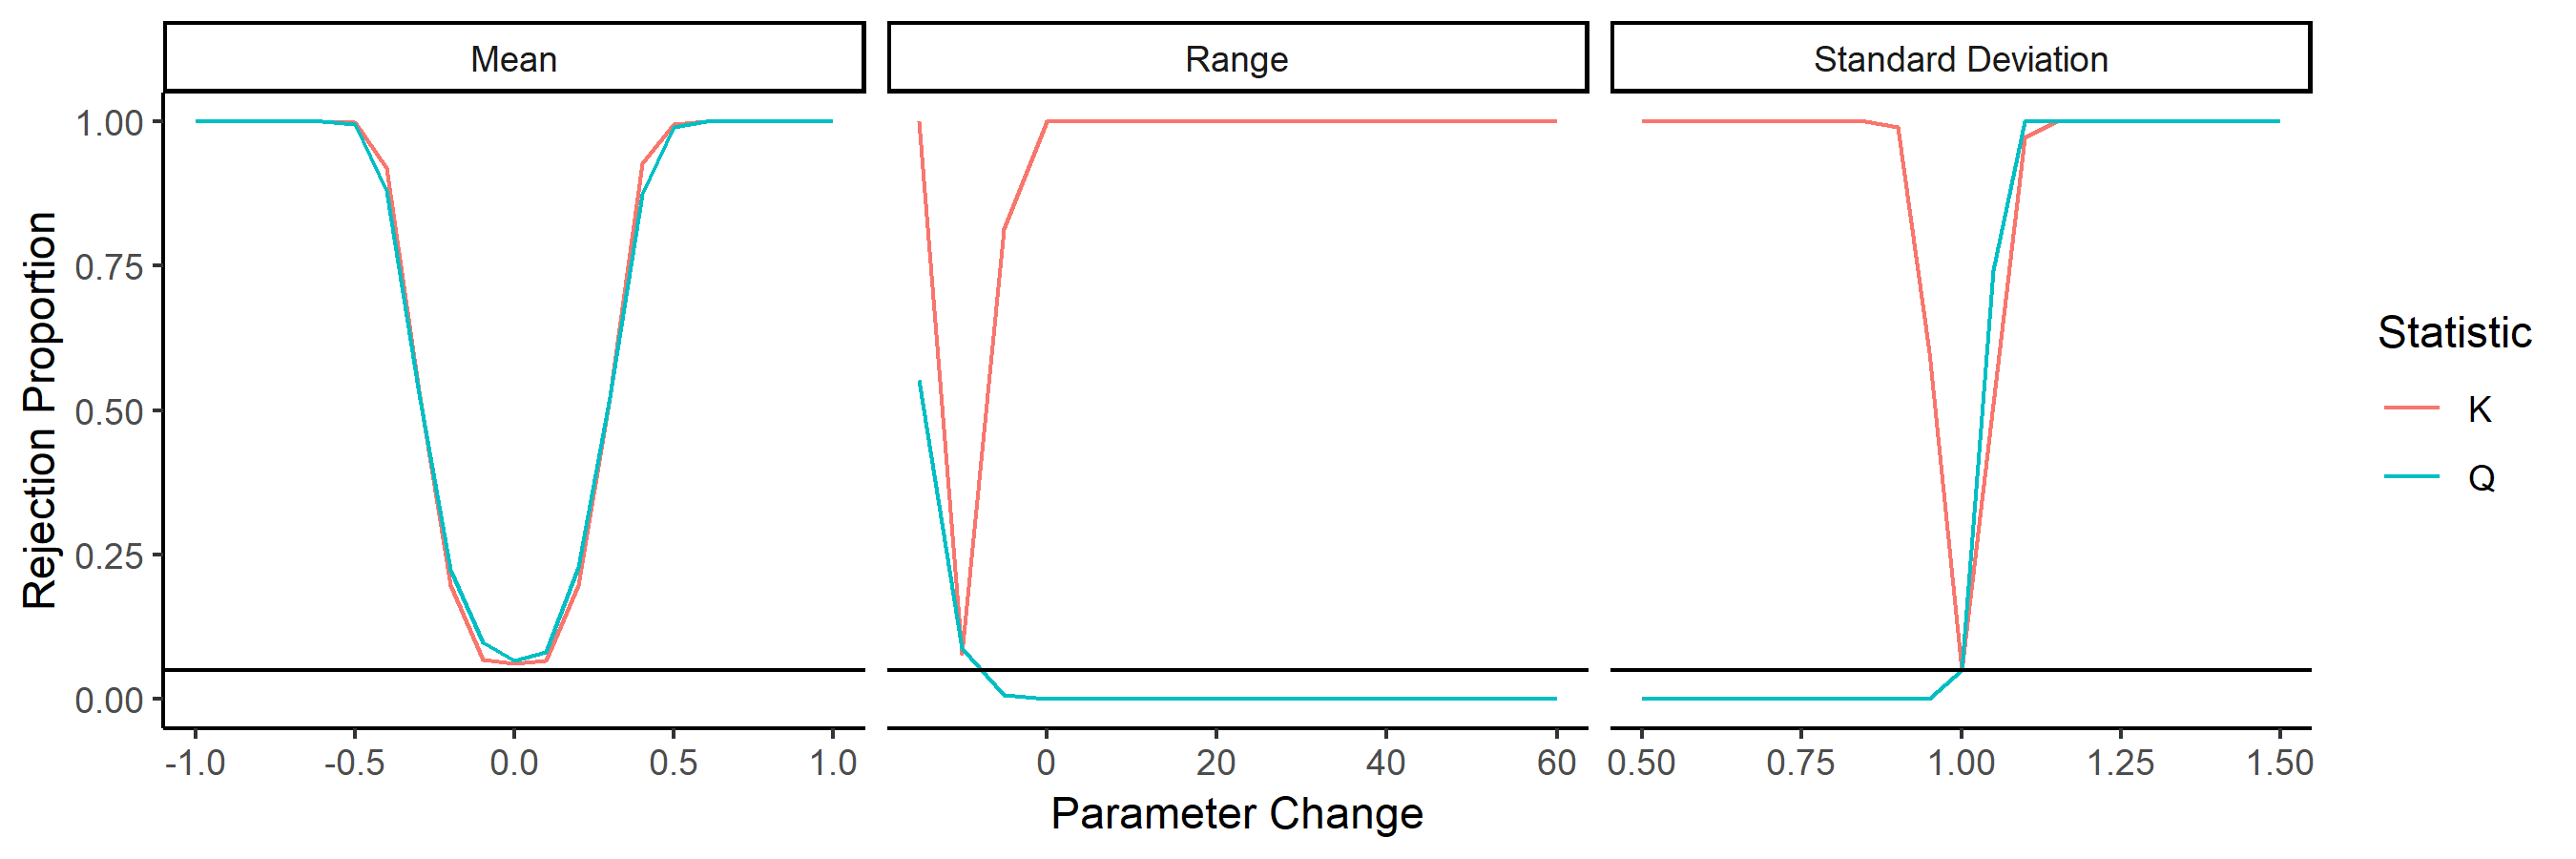
\includegraphics[width=0.8\textwidth,valign=c]{power/multi2d2.png}
    \caption{Power of $K$ and $QI$ in detecting changes in the three parameters in Gaussian process. Mean and Range are presented as shifts of parameters in $Y$ from $X$. Standard Deviation is presented as a multiple of standard deviation in $X$.}
    \label{power2d2}
    \end{center}
\end{figure}

% \begin{figure}
% 	\begin{center}
%     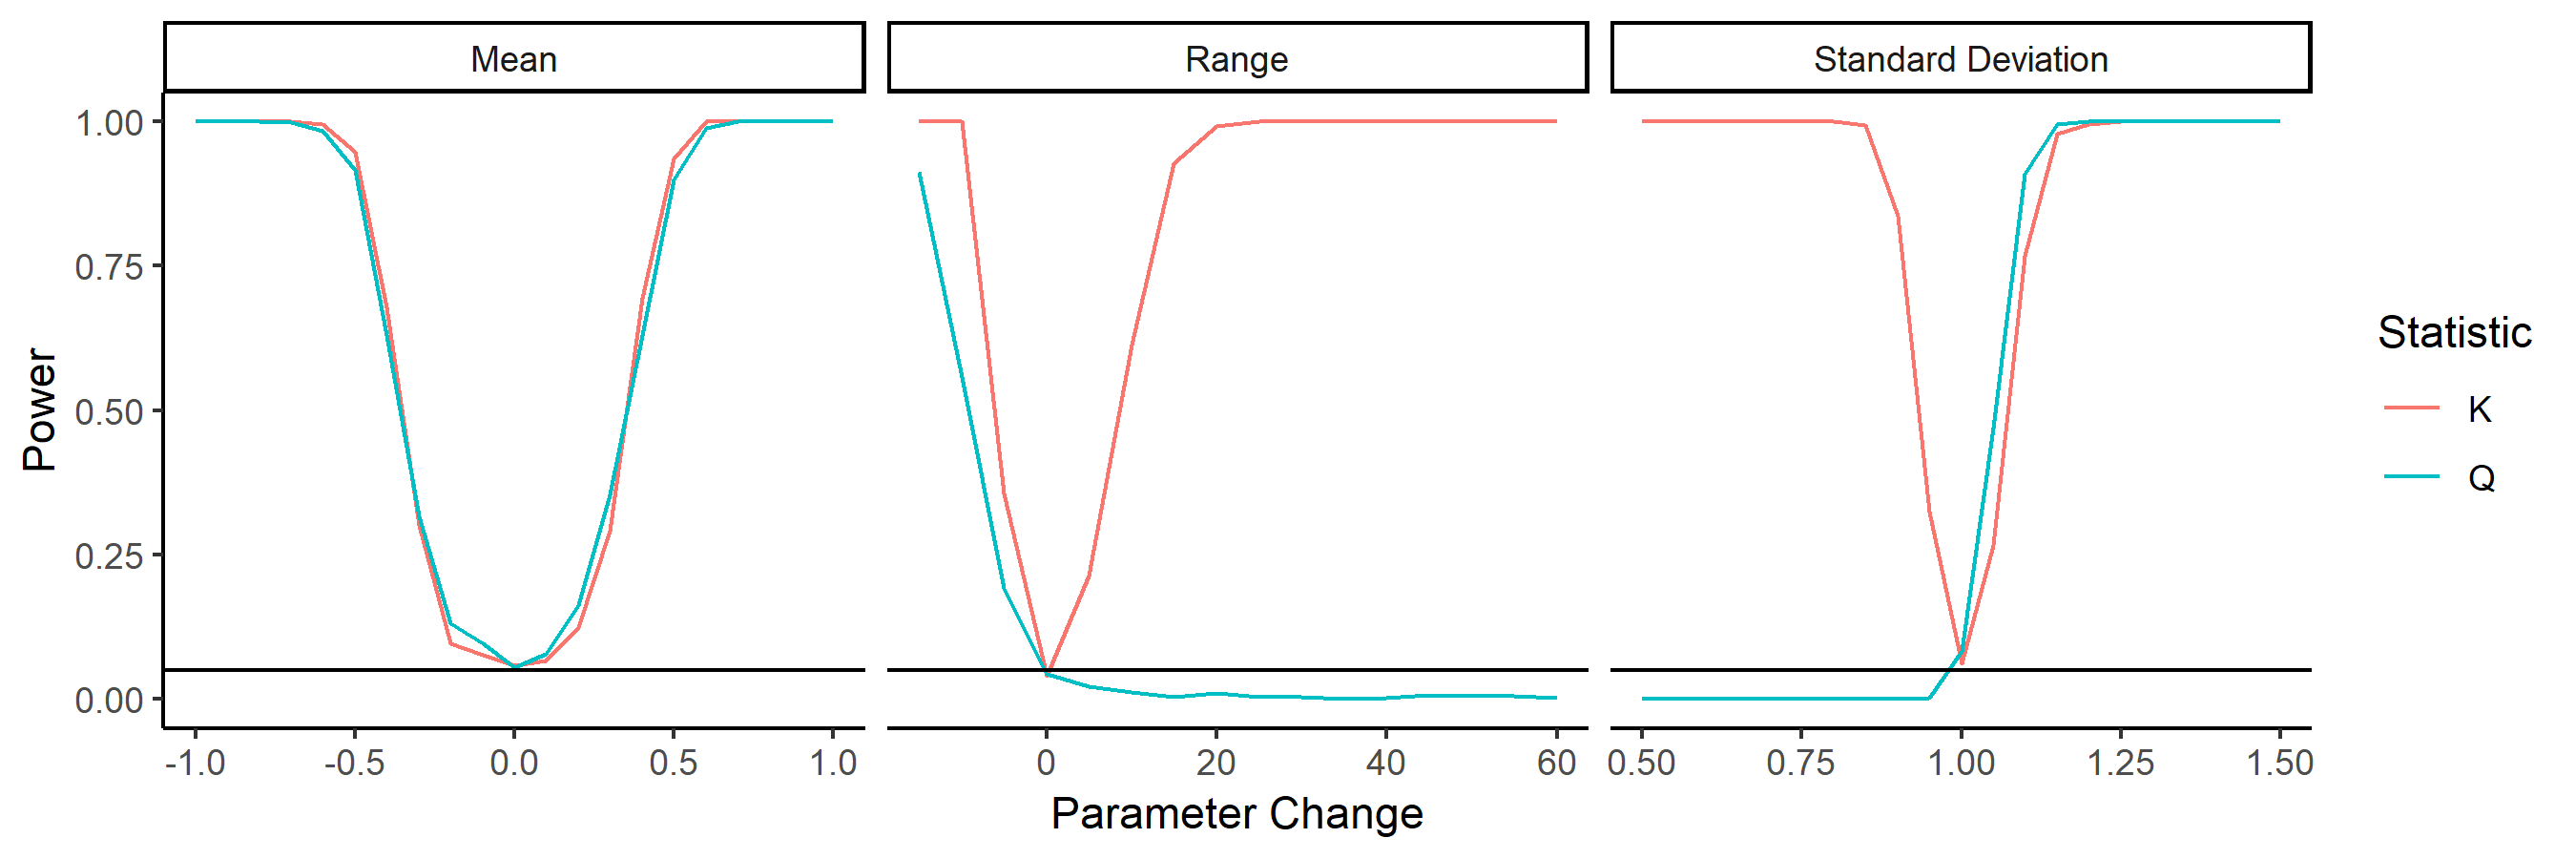
\includegraphics[width=0.8\textwidth,valign=c]{power/multi2d.png}
%     \caption{Power of $K$ v.s. $QI$ to detect changes in the three Gaussian process parameters on 2D data. Mean and Range are presented as shifts in $Y$'s corresponding parameter from $X$. Standard Deviation is presented as a multiple of $X$'s standard deviation.}
%     \label{power2d}
%     \end{center}
% \end{figure}

Figure \ref{power2d2} shows power functions for each parameter when $X$ has $r = 10$. Full results can be found in the Appendix.  Essentially, increasing the smoothness only flattens the power function slightly. Both $K(X, Y)$ and $QI$ are almost equally powerful in detecting changes in mean, decreases in range, and increases in standard deviation. However, $K(X, Y)$ shows improvement over $QI$ in detecting increases in range or decreases in standard deviation. It should be noted that $QI$ was explicitly designed to ignore decreases in standard deviation, since in their application a drop in standard deviation was desirable.

The situation where the mean or variance is shifted uniformly over the entire domain of the function may be a little too simplified. A more realistic scenario is that the mean, variance, and other aspects of the distribution differ heterogeneously; higher in some regions and lower in others. To study this situation we conduct another set of simulations where the mean and variance are both allowed to vary non-uniformly over the domain, though the range is kept constant throughout at $r = 20$. More specifically, we  generate the mean and standard deviation of $Y$ as two dimensional sine waves centered about 0 and 1, respectively.  Then we slowly increase the amplitude of sine waves to make $X$ and $Y$ deviate more in their parameters. The two sine waves were generated as follows:
\begin{align*}
    \mu(s) &= t \sin \left( 2 \pi \frac{s_1}{20} \right) \otimes t \sin \left( 2 \pi \frac{s_2}{20} \right)\\
    \sigma(s) &=  t \sin \left(2 \pi \frac{s_1}{20} \right) \otimes t \sin \left(2 \pi \frac{s_2}{20} \right) + 1,
\end{align*}
\bl{why there are four equations?}
\begin{align*}
    \mu(s) &= \left(0.8 t \cos \left(\pi \frac{s_1}{20} \right) + 1 \right) \otimes \left(0.8 t \cos \left(\pi \frac{s_1}{20} \right) + 1 \right) - 1 \\
    \sigma(s) &=  \left(0.8 t \cos \left(\pi \frac{s_1}{20} \right) + 1 \right) \otimes \left(0.8 t \cos \left(\pi \frac{s_1}{20} \right) + 1 \right), \\
\end{align*}
where $s = (s_1, s_2)$ and $t$ was varied from 0.05 to 1 in increments of 0.05. We fixed the sample size to $n = 500$ and used 1000 simulations per $t$ value to estimate the power at $t$.

Figure \ref{power2dstoch} shows the power functions of $K$ and $QI$ under heterogeneous mean and standard deviation changes. For detecting mean changes, both $K$ and $QI$ maintain comparable powers although our test indeed carries more power than the $QI$ test at certain range of mean change. It is worth noting that the power curves in this setting appear to be similar to those under the homogeneous mean change which indicates no serious power loss when the mean change is heterogeneous. However, huge difference between $K$ and $QI$ is observed when the standard deviation change is heterogeneous. Basically, $K$ still completely maintains its power while $QI$ fails. 

 

% This time we view the process $X$ as having a constant mean function $\mu = 0$ over its whole domain and instead of shifting the mean of the $Y$ process by some fixed increment we sample Gaussian processes with progressively larger variances. The Gaussian process used to generate $Y$'s mean had a $\mu = 0$, $r = 20$ a $\sigma$ that was allowed to vary from 1 to 2 in increments of 0.05. The random mean was then centered at $1$ so that the increase in $\sigma$ would correspond to more variability in the mean function of $Y$. The rejection proportion for $K$ and $QI$ were the computed and plotted them against the $L^2$ distance between their means, Fig. \ref{power2dstoch}. This time we fixed the sample size to $n = 200$, the range $r  = 20$, and the number of simulations per setting to $1000$. The power function for $K$ remains largely unchanged from the constant shift case, but there is a slight drop in power for $QI$.

% Simulating non uniform standard deviation changes took a little more care. This time we greatly increased the correlation in the Gaussian process which generates $Y$'s standard deviation function by setting $r = 200$. Because of the correlations within the functions of $Y$, small irregular changes in variance are washed out so a noisy Gaussian process for $\sigma$ centered at 1 will be undetectable. Persistent changes in variance are detectable though which is what increasing the range parameter accomplishes. Figure \ref{power2dstoch} shows the power functions of $K$ and $QI$ against the $L^2$ distance between $X$ and $Y$'s variance functions. Again we fixed the sample size to $n = 200$, the range $r  = 20$, and the number of simulations per setting to $1000$. Figure \ref{power2dstoch} reports the associated rejection proportions of $K$ and $QI$. $K$ maintains its power under the non constant change regime but $QI$ experiences a total loss in power.

\begin{figure}
	\begin{center}
    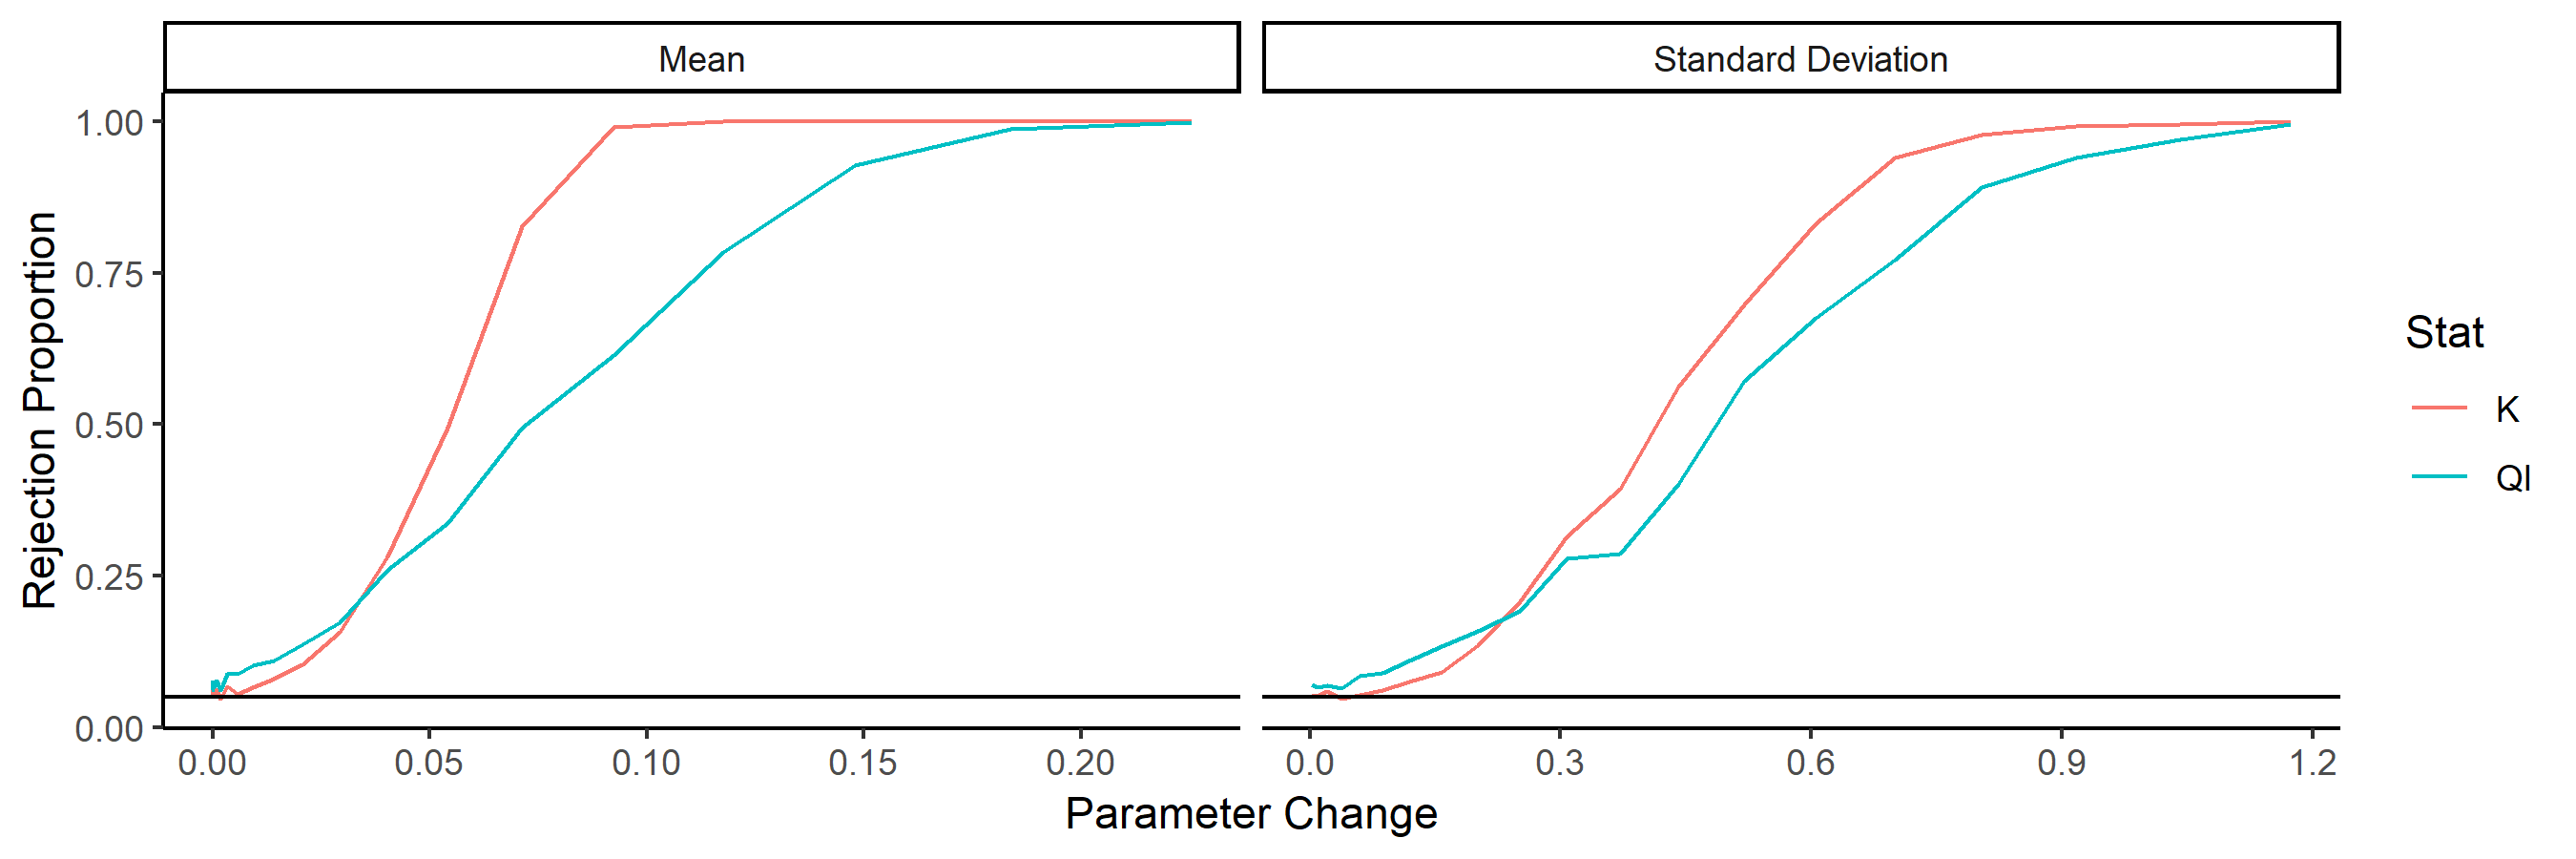
\includegraphics[width=0.8\textwidth,valign=c]{power/multi_het.png}
    \caption{Power functions for $K$ and $QI$ under heterogeneous differences in the mean and standard deviation between $X$ and $Y$. Powers were plotted against the $L^2$ distance in the mean and standard deviation between $X$ and $Y$.}
    \label{power2dstoch}
    \end{center}
\end{figure}


% \begin{figure}
%   \subfloat{%
%     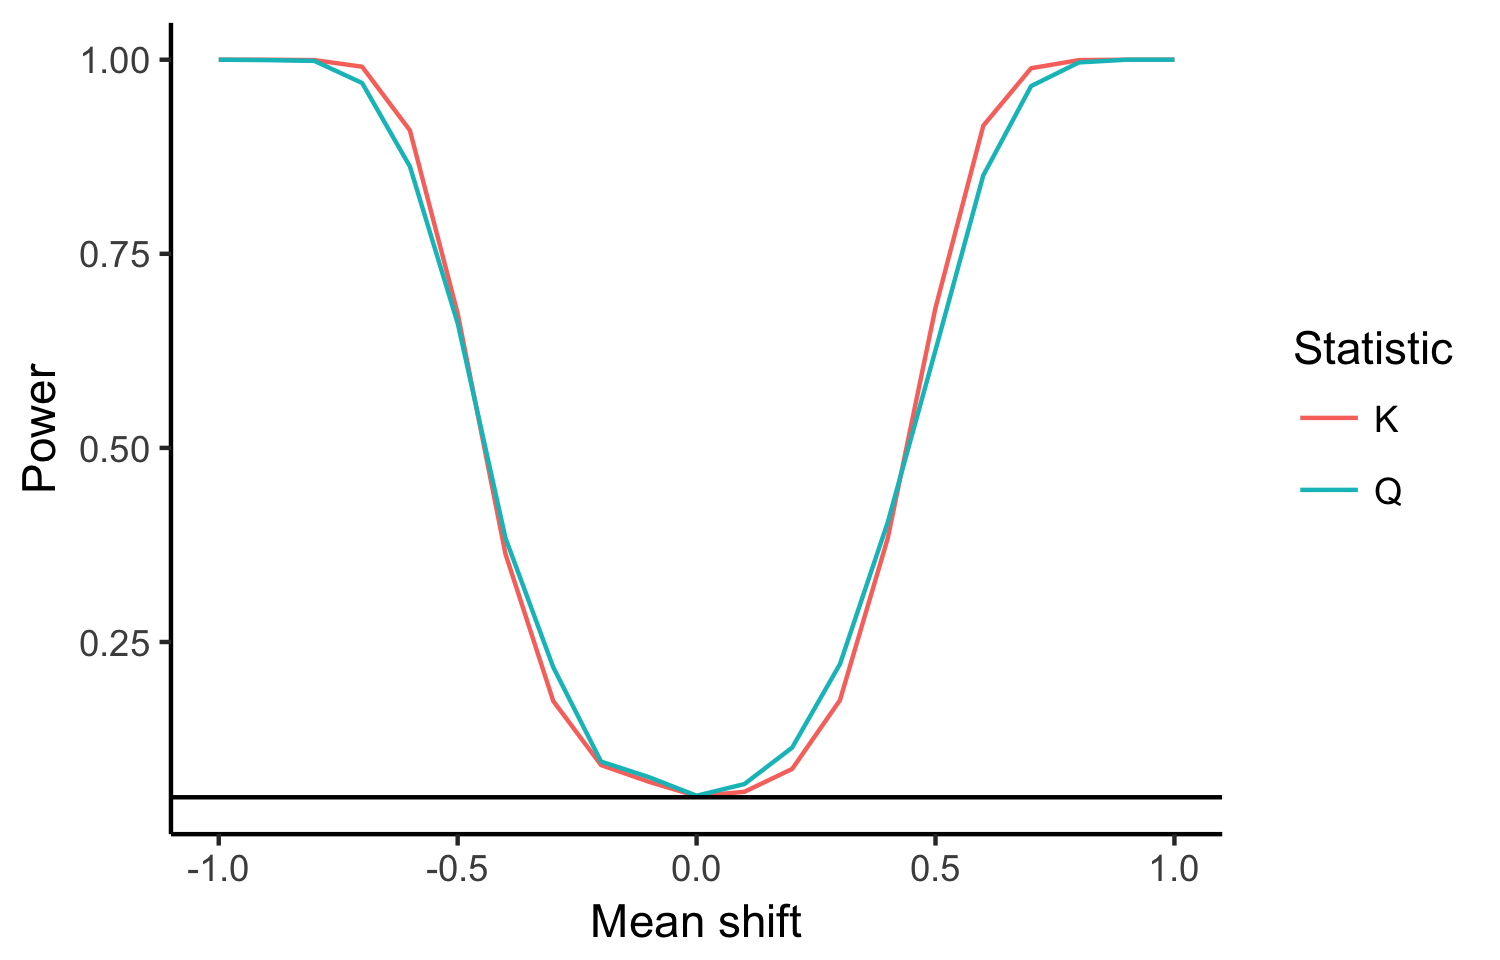
\includegraphics[width=0.50\textwidth,valign=c]{power/location1d.png}
%   }
%   \subfloat{%
%     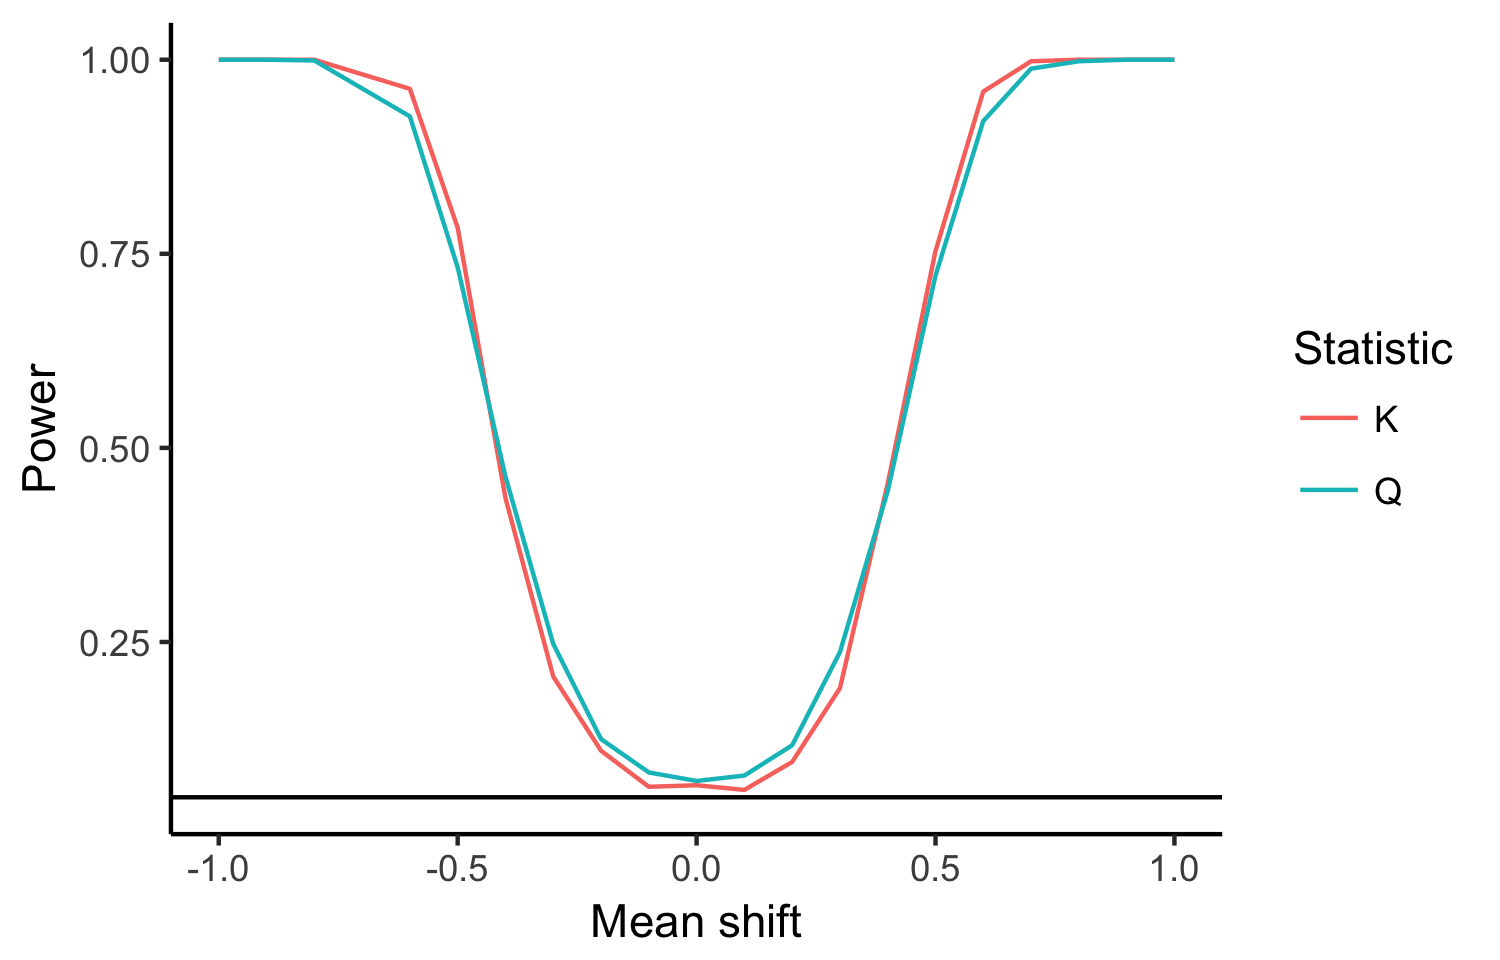
\includegraphics[width=0.50\textwidth,valign=c]{power/location.png}
%   }
%   \caption{Power (mean) for 1D functions (left) and 2D functions (right)}
% \end{figure}

% \begin{figure}
%   \subfloat{%
%     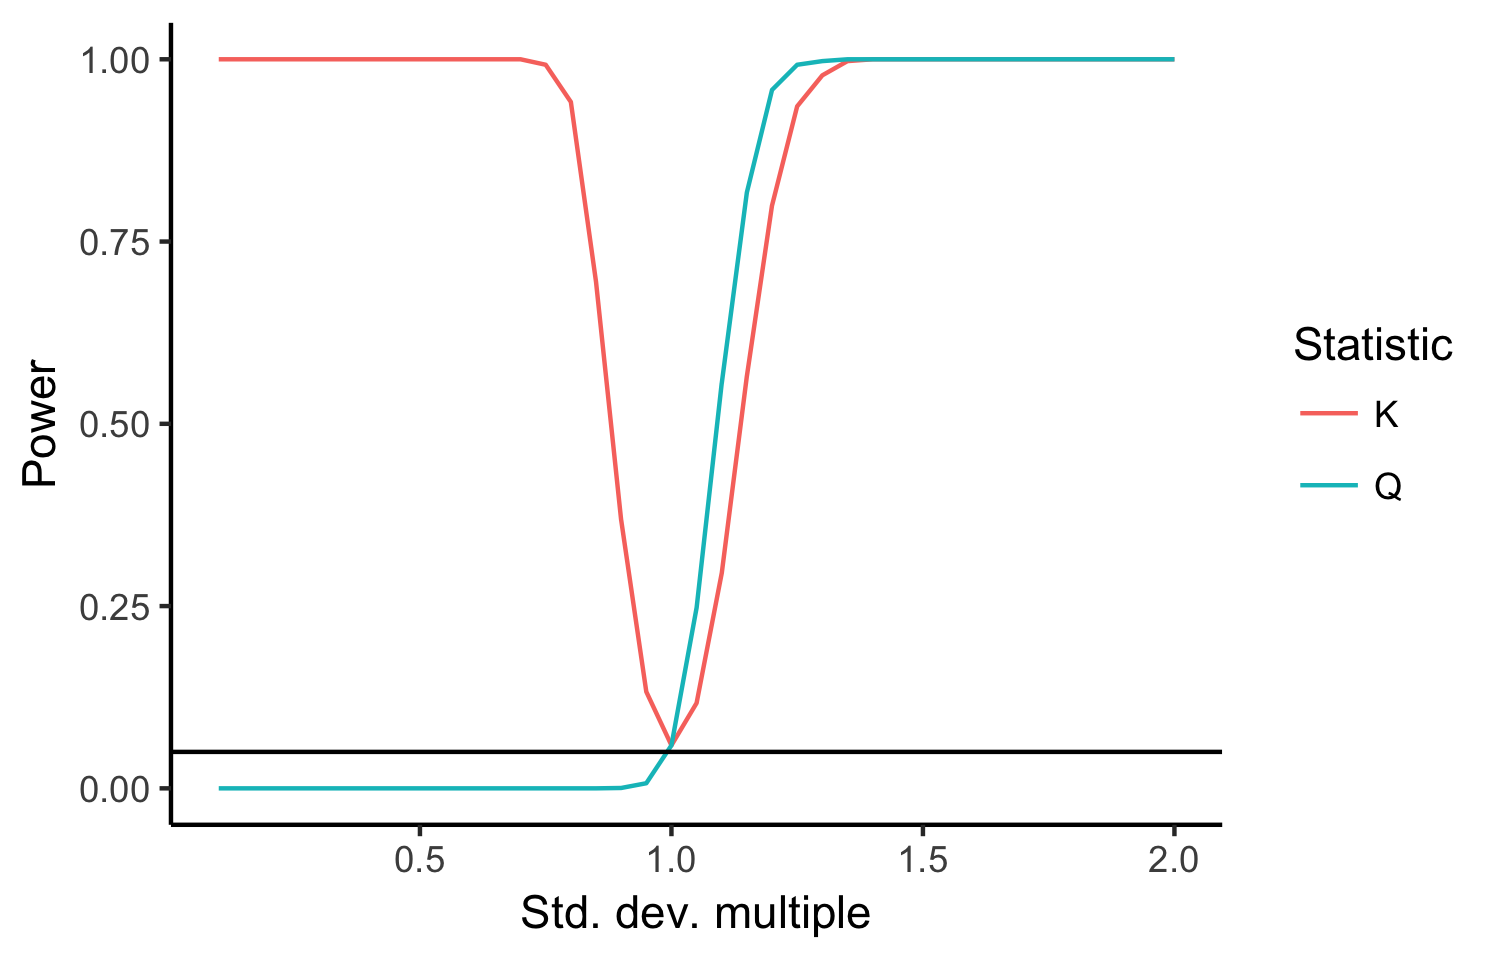
\includegraphics[width=0.50\textwidth,valign=c]{power/scale1d.png}
%   }
%   \subfloat{%
%     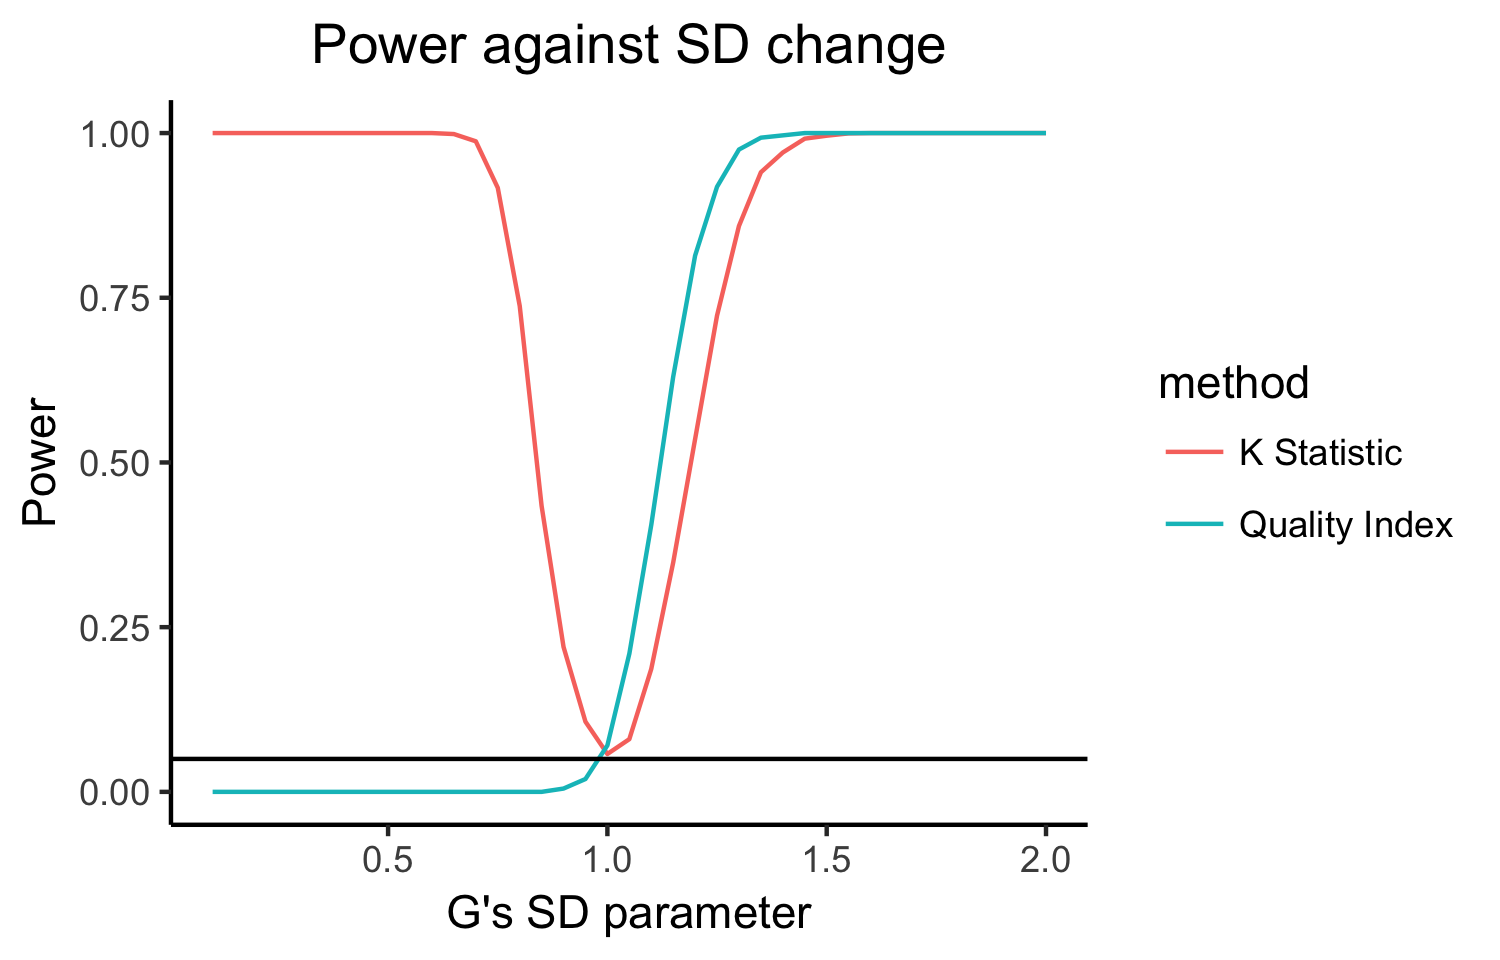
\includegraphics[width=0.50\textwidth,valign=c]{power/scale.png}
%   }
%   \caption{Power (scale) for 1D functions (left) and 2D functions (right)}
% \end{figure}

% \begin{figure}
%   \subfloat{%
%     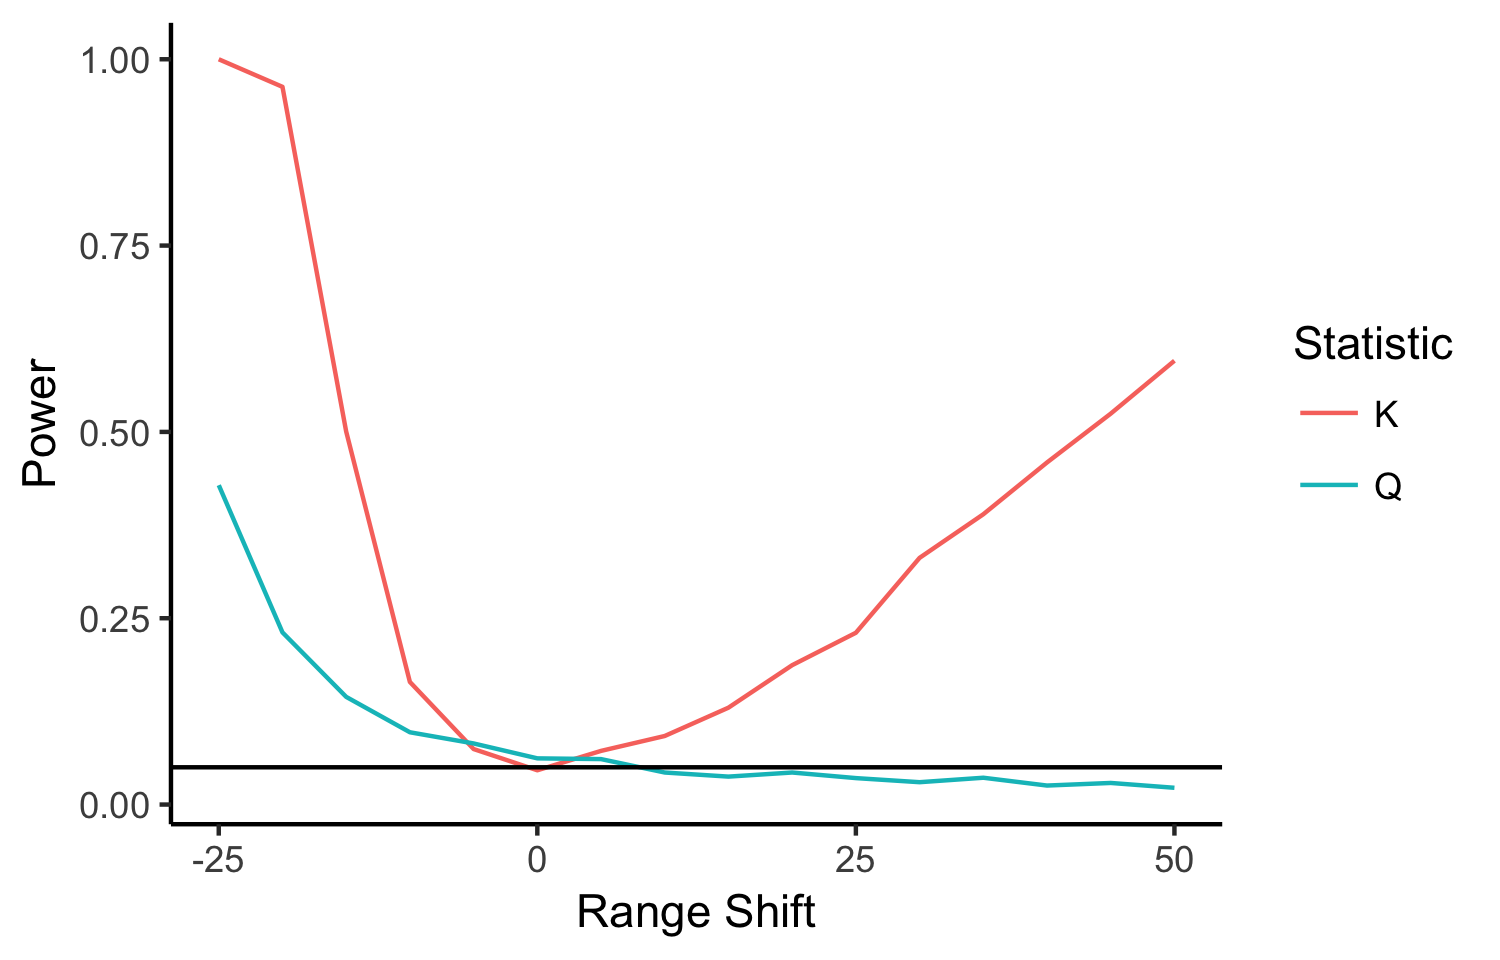
\includegraphics[width=0.50\textwidth,valign=c]{power/correlation1d.png}
%   }
%   \subfloat{%
%     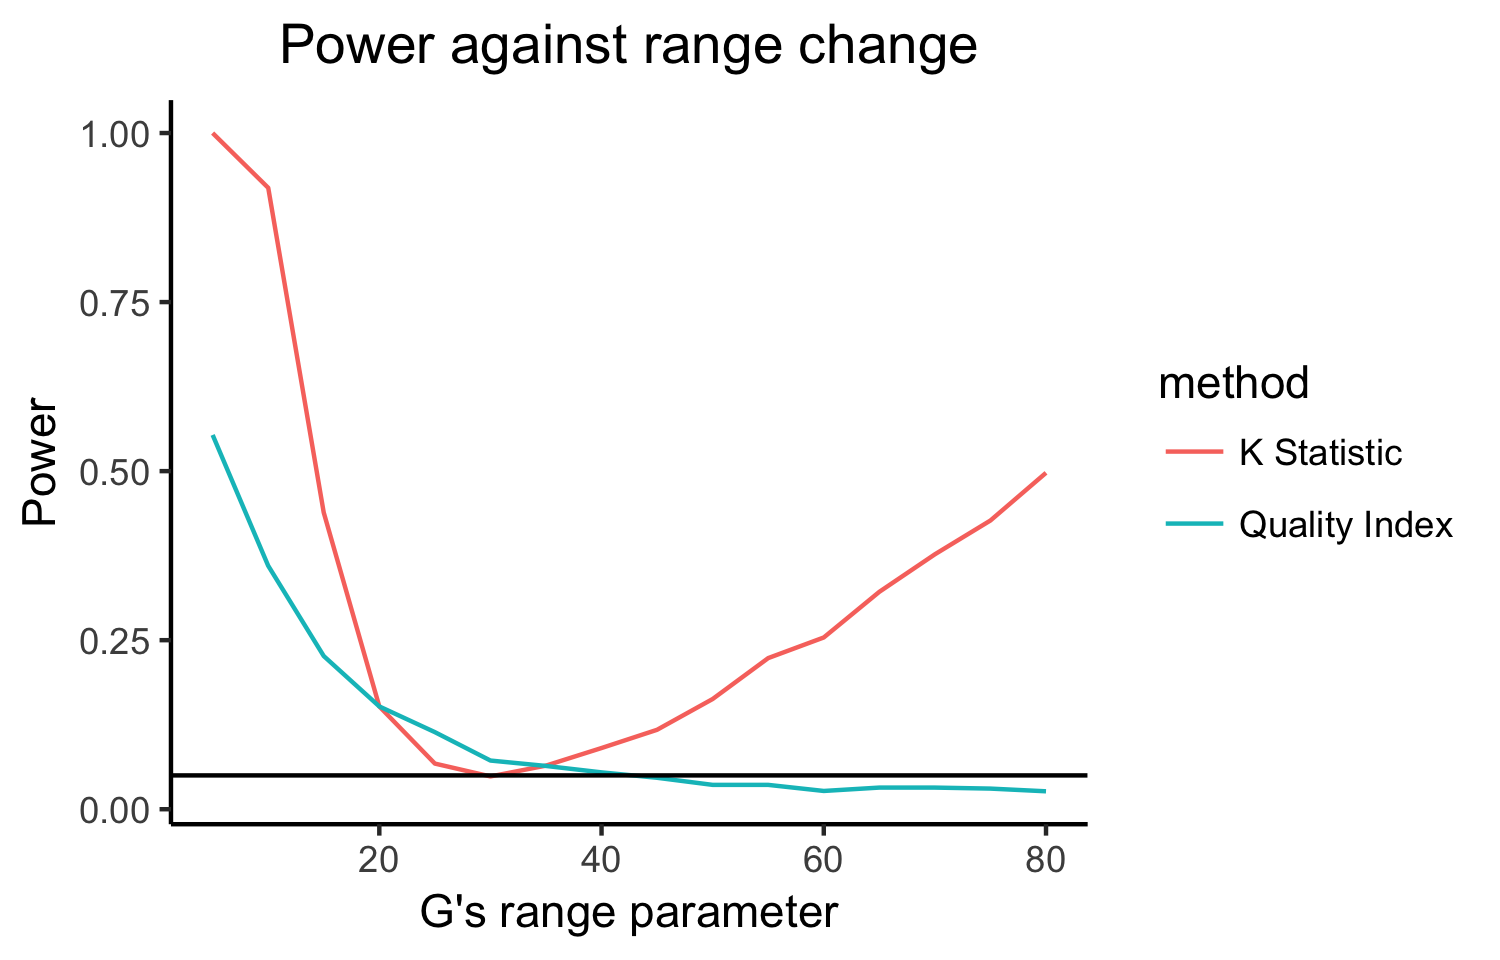
\includegraphics[width=0.50\textwidth,valign=c]{power/correlation.png}
%   }
%   \caption{Power (correlation) for 1D functions (left) and 2D functions (right)}
% \end{figure}


% \begin{figure}
%   \subfloat{%
%     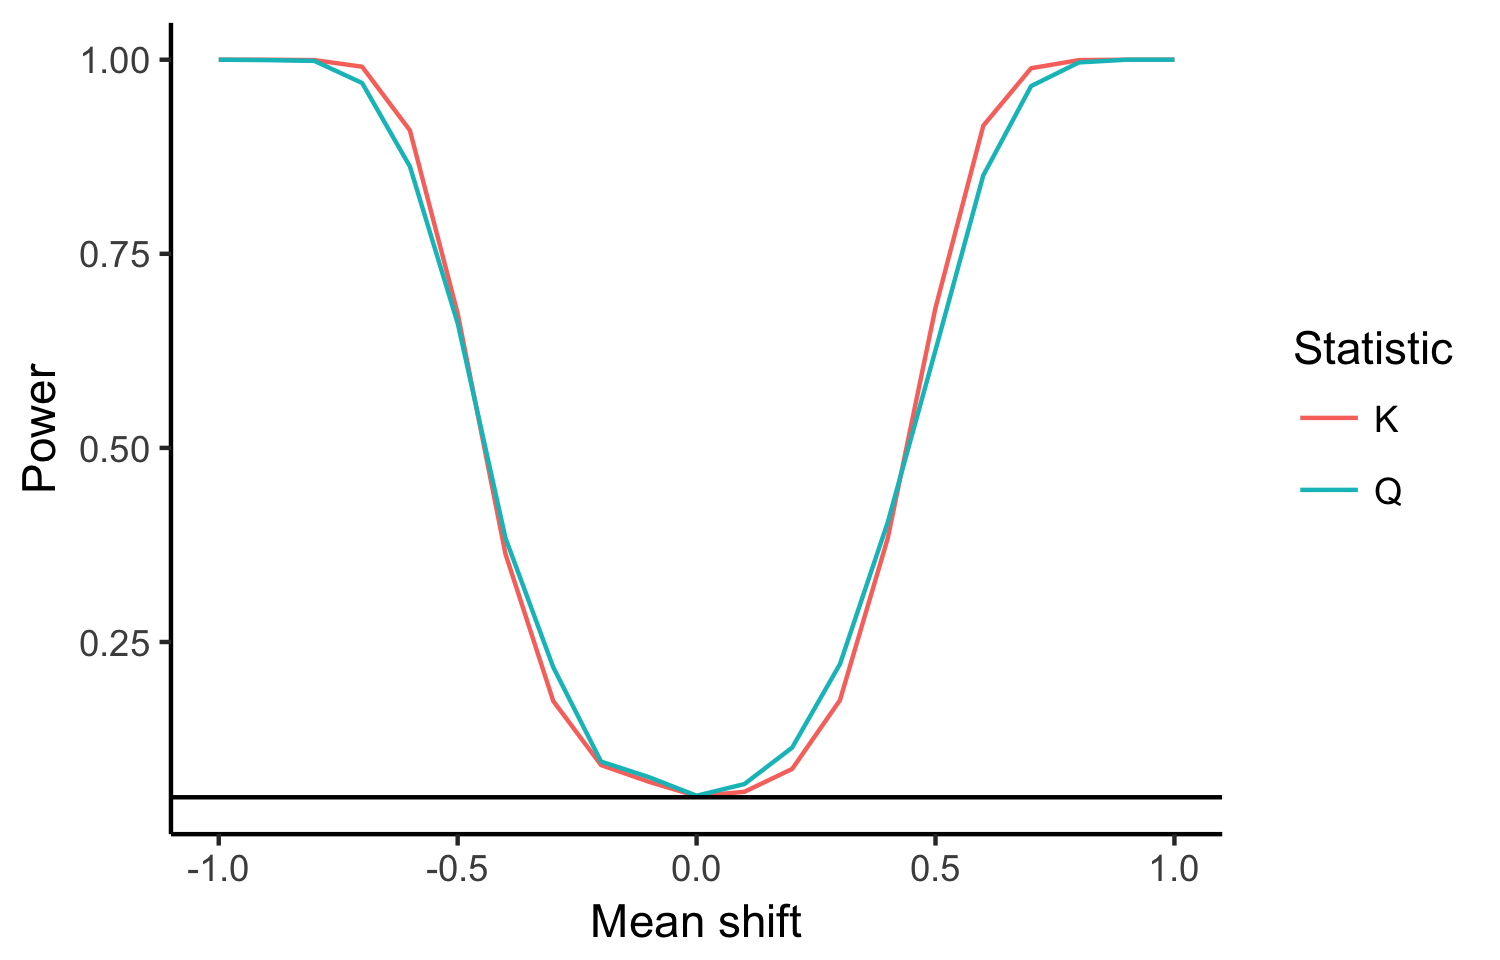
\includegraphics[width=0.3\textwidth,valign=c]{power/location1d.png}
%   }
%   \subfloat{%
%     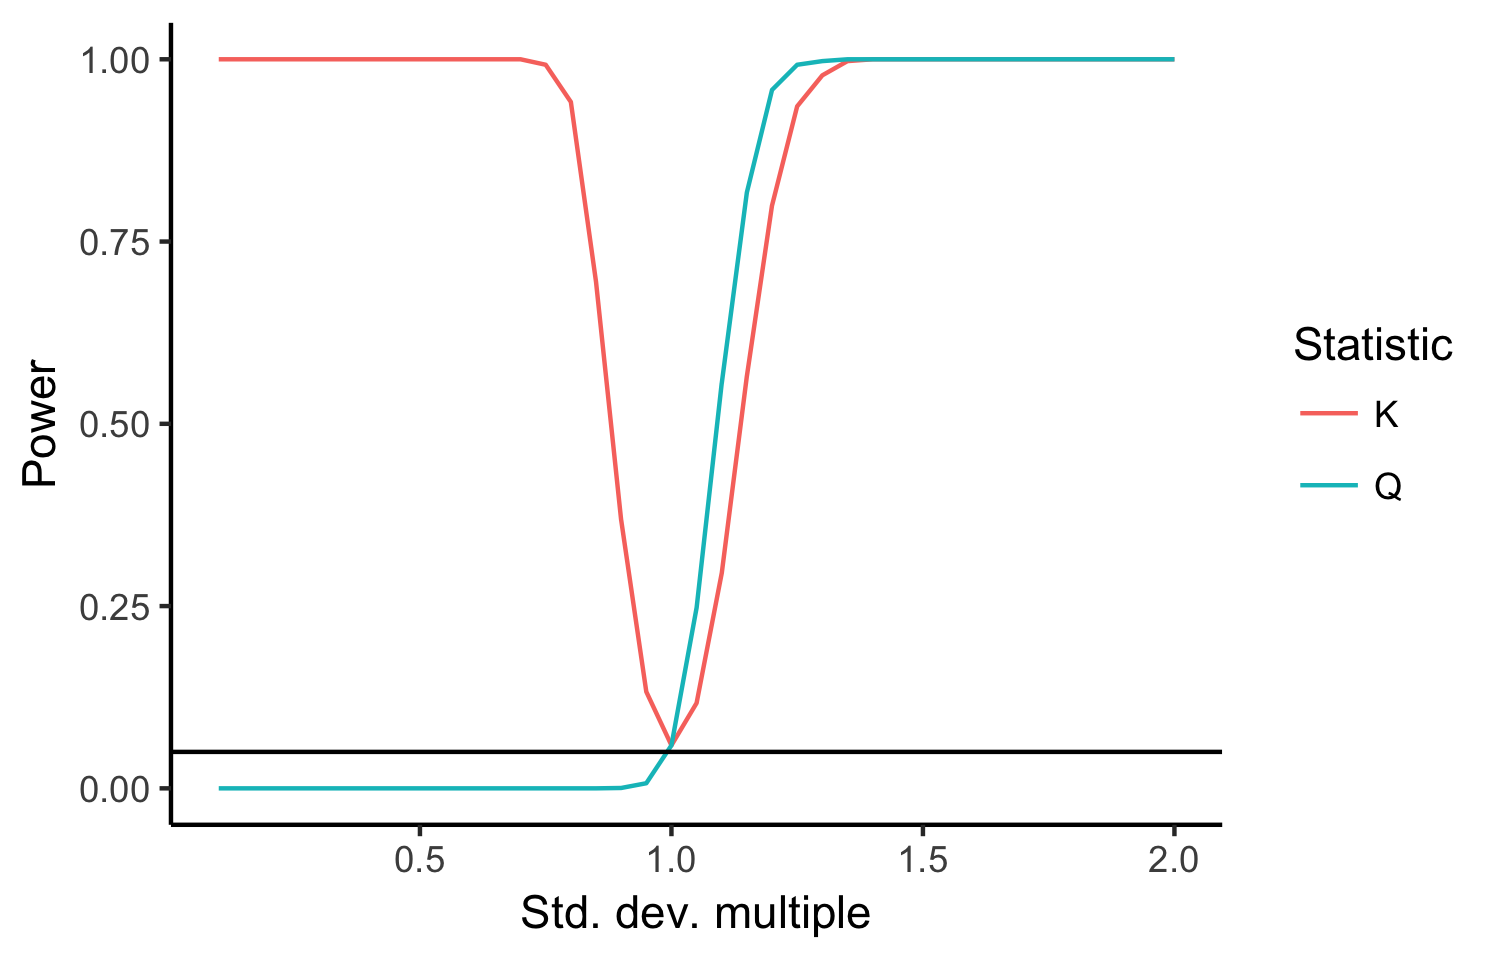
\includegraphics[width=0.3\textwidth,valign=c]{power/scale1d.png}
%   }
%   \subfloat{%
%     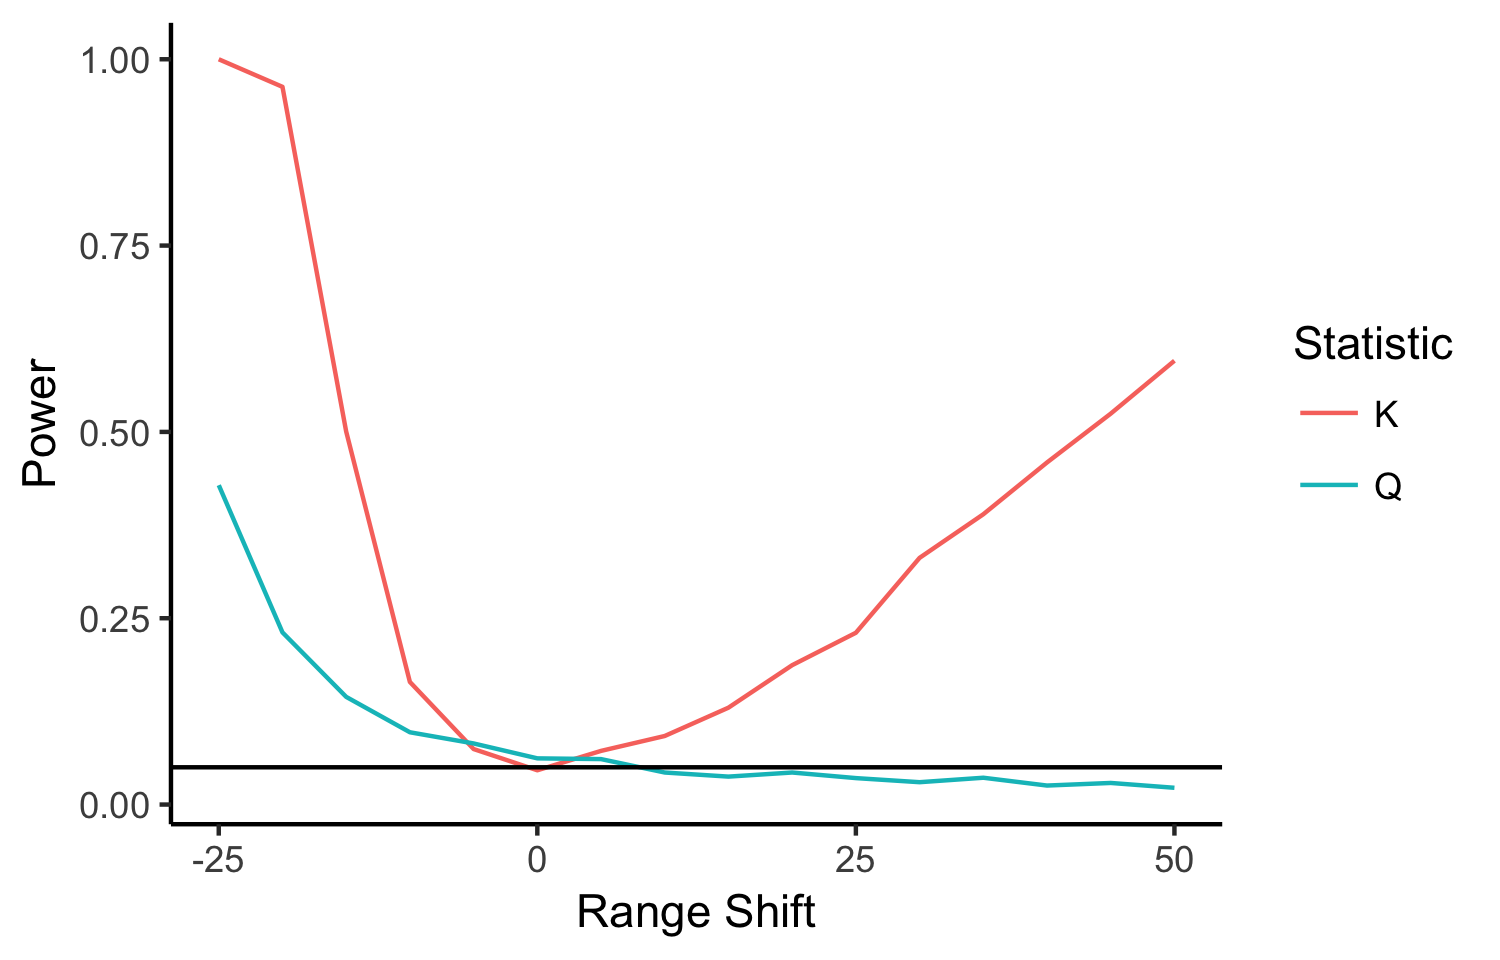
\includegraphics[width=0.3\textwidth,valign=c]{power/correlation1d.png}
%   } \\
%   \subfloat{%
%     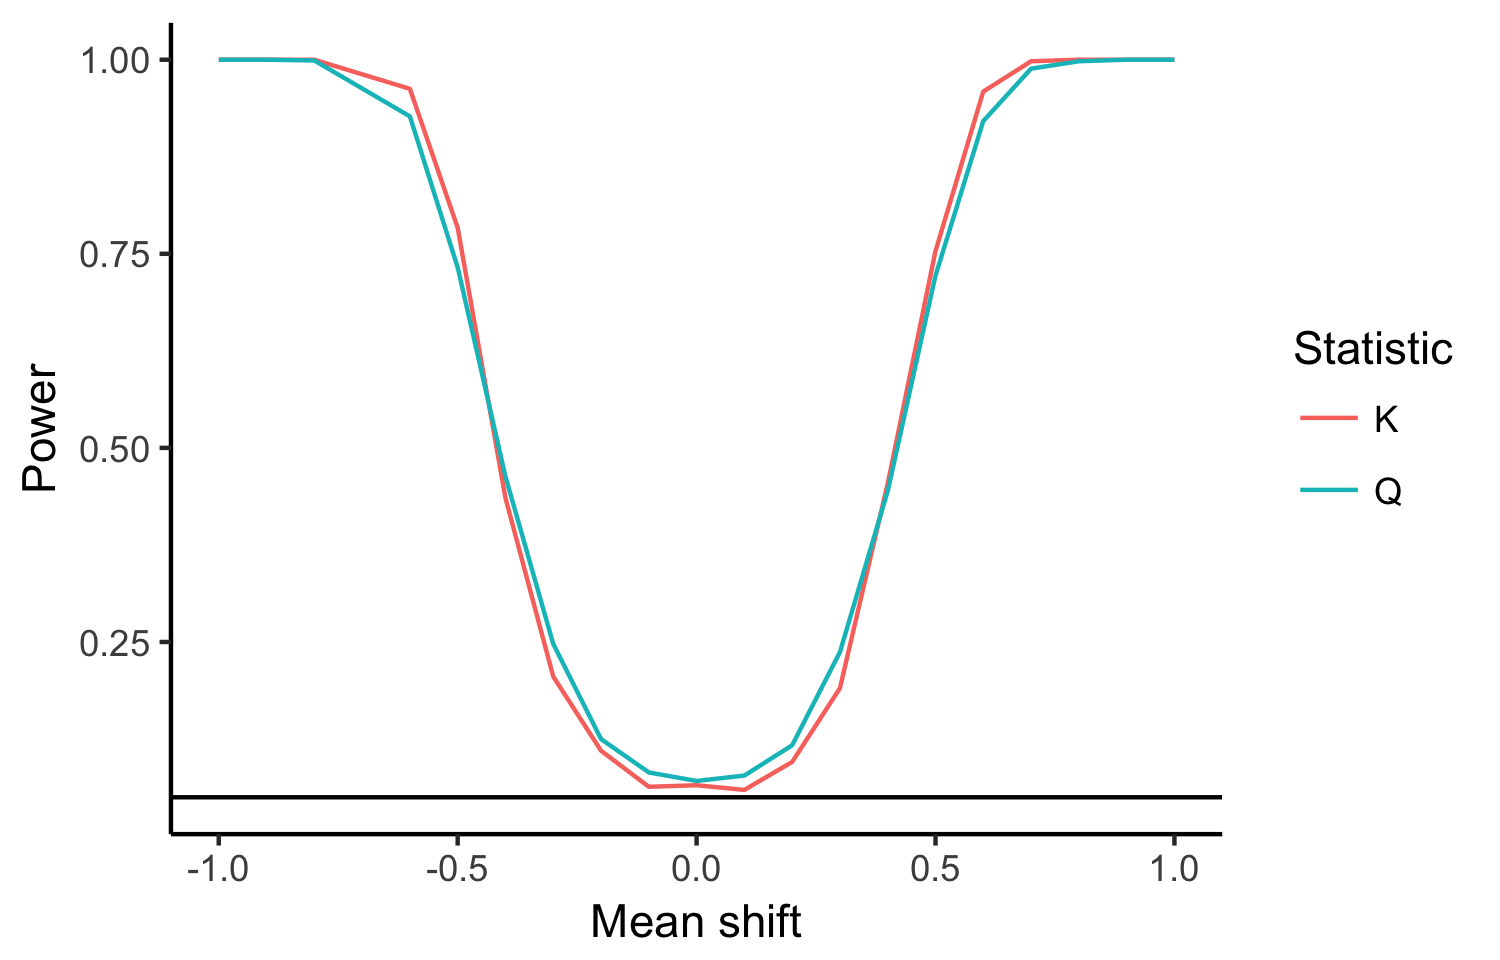
\includegraphics[width=0.3\textwidth,valign=c]{power/location.png}
%   }
%   \subfloat{%
%     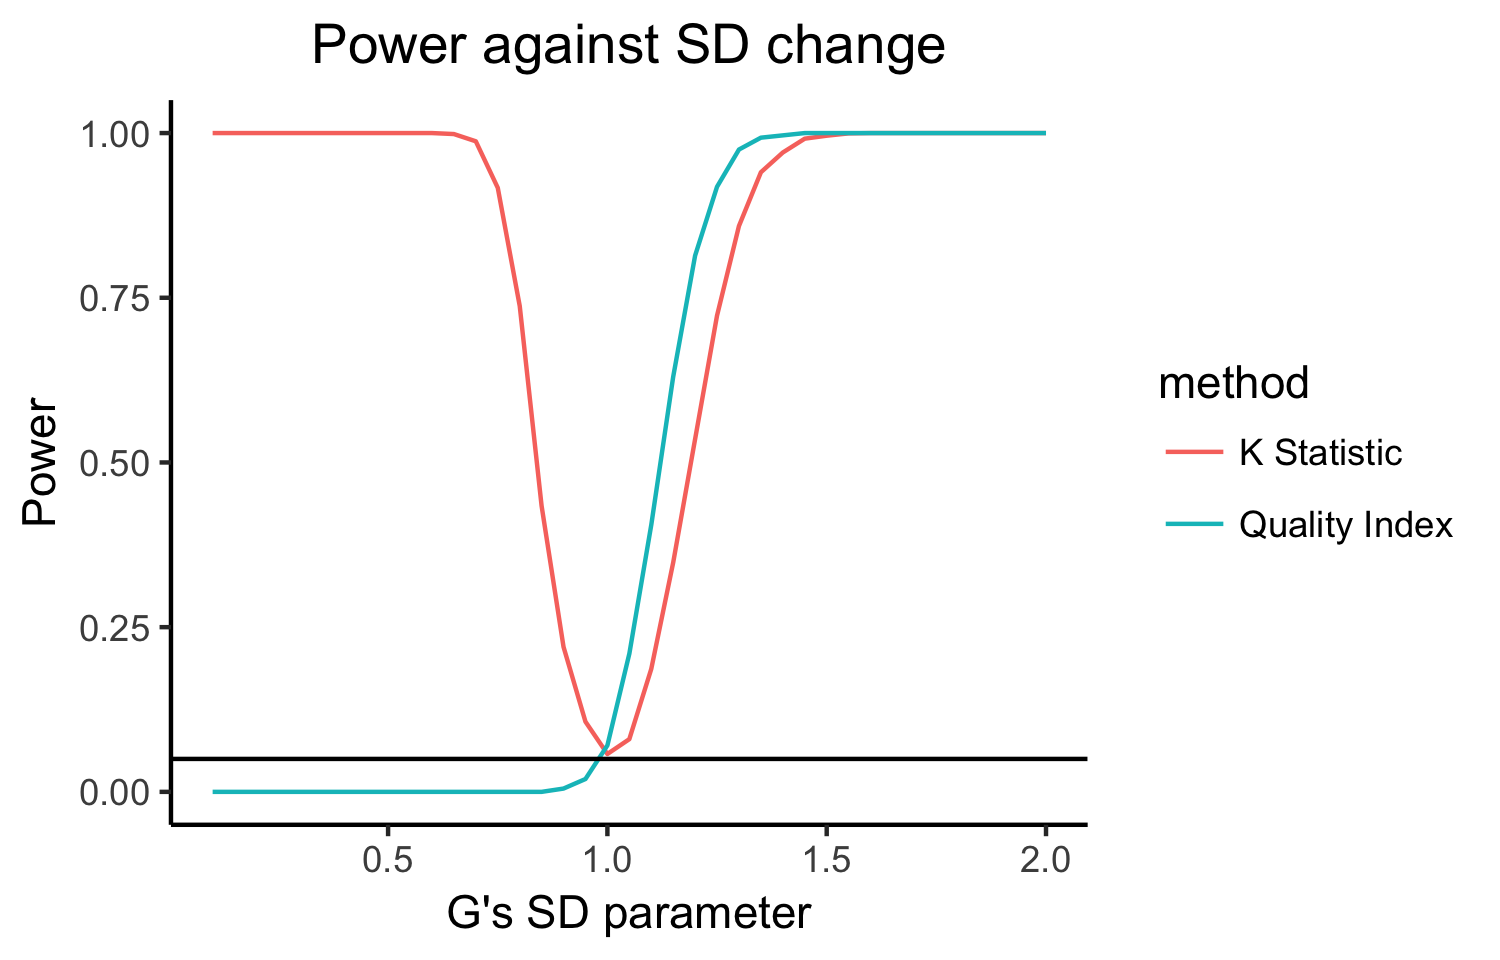
\includegraphics[width=0.3\textwidth,valign=c]{power/scale.png}
%   }
%   \subfloat{%
%     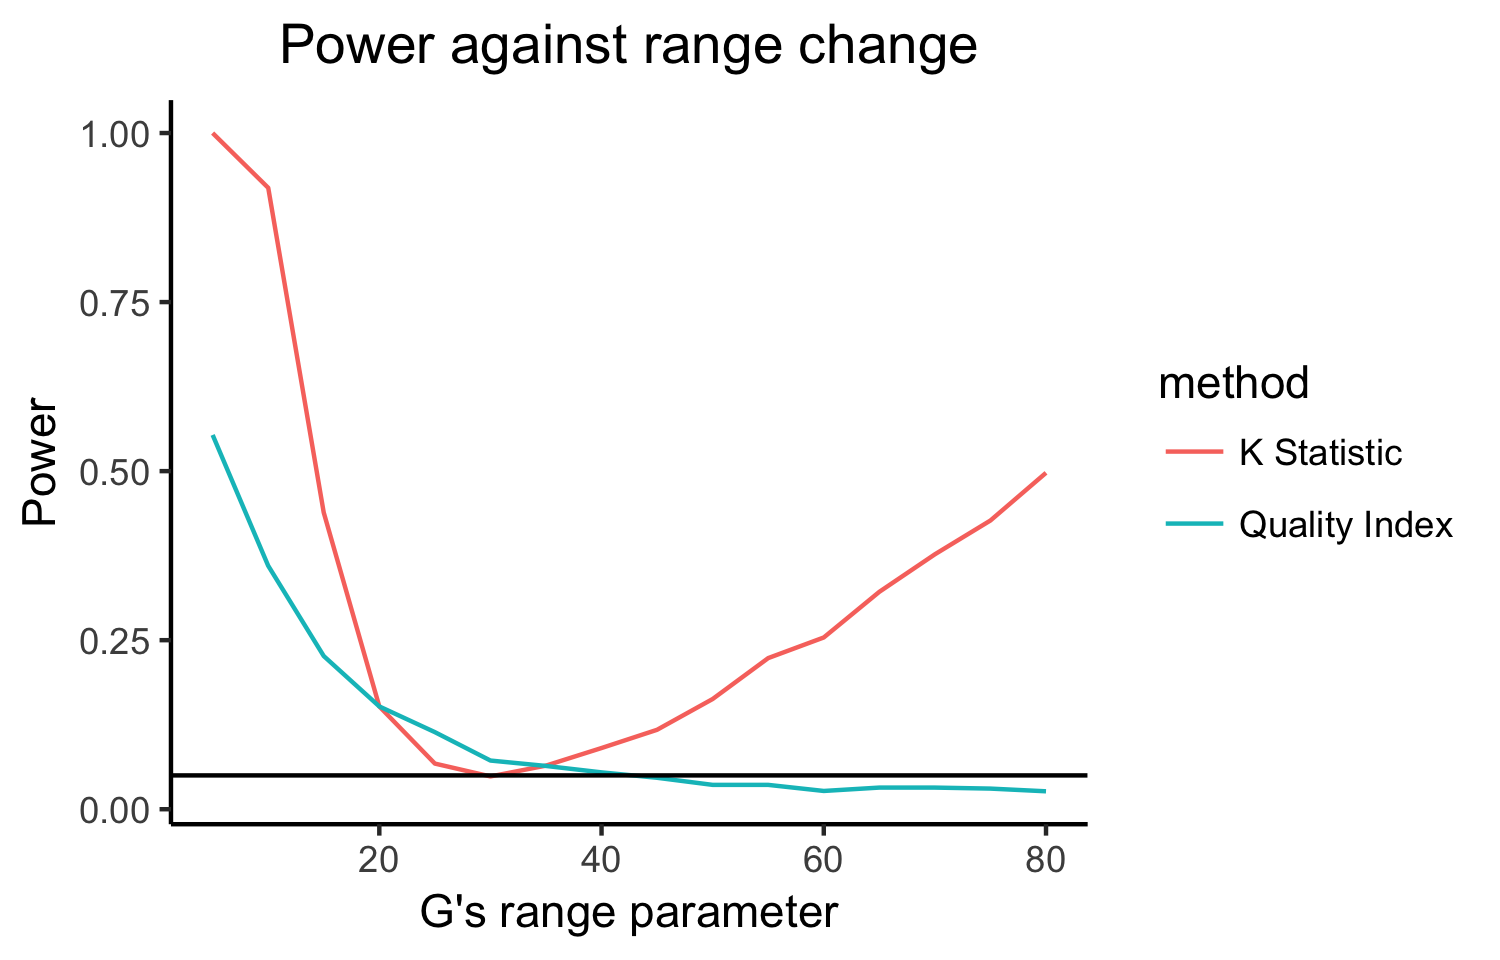
\includegraphics[width=0.3\textwidth,valign=c]{power/correlation.png}
%   }
%   \caption{Power (mean) for 2D functions (left) and 2D functions (right)}
% \end{figure}


%%%%%%%%%% APPLICATION
\section{Application to Data Assimilation} \label{app}

We used the proposed test $K$ to detect differences in the background and analysis states of the 1000 year two meter surface temperature reconstruction. Differences at the global level are investigated in section \ref{global} using the full spatial extent of the background and analysis states. In section \ref{regional} the background and analysis are partitioned into 12 regions corresponding to the 5 oceans and 7 continents. We investigate how differences at the global level distribute down to these regions and how correlation between regions may impact $K$.

\subsection{Global Reconstructions} \label{global}

\begin{figure}
  \centering
  \subfloat{%
    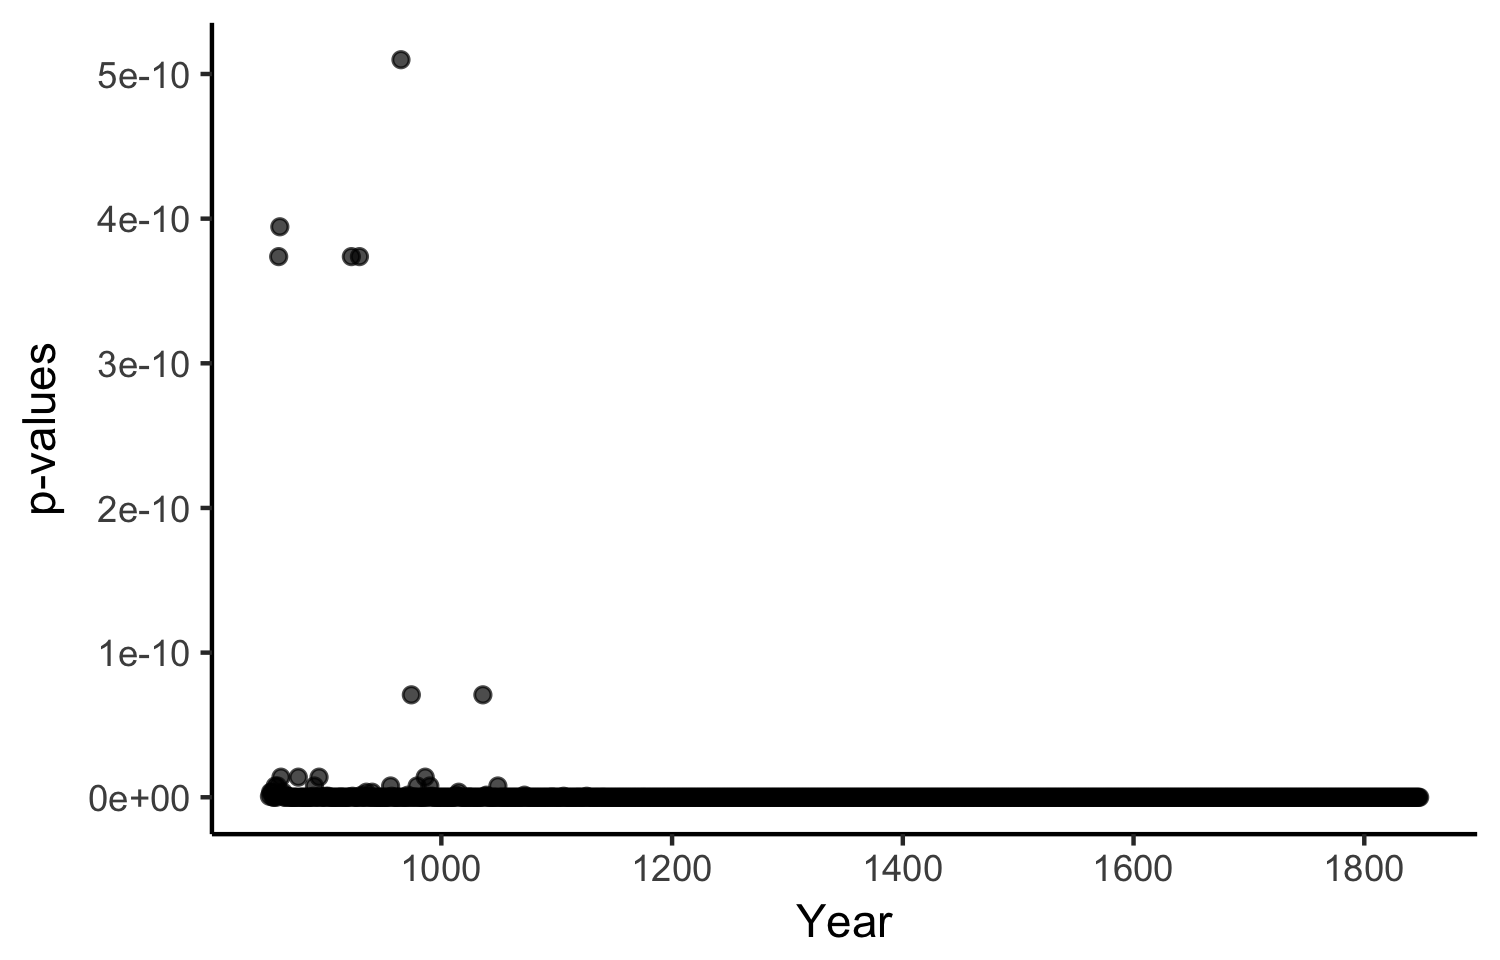
\includegraphics[width=0.45\textwidth]{results/pval_over_time.png}
  }
  \subfloat{%
    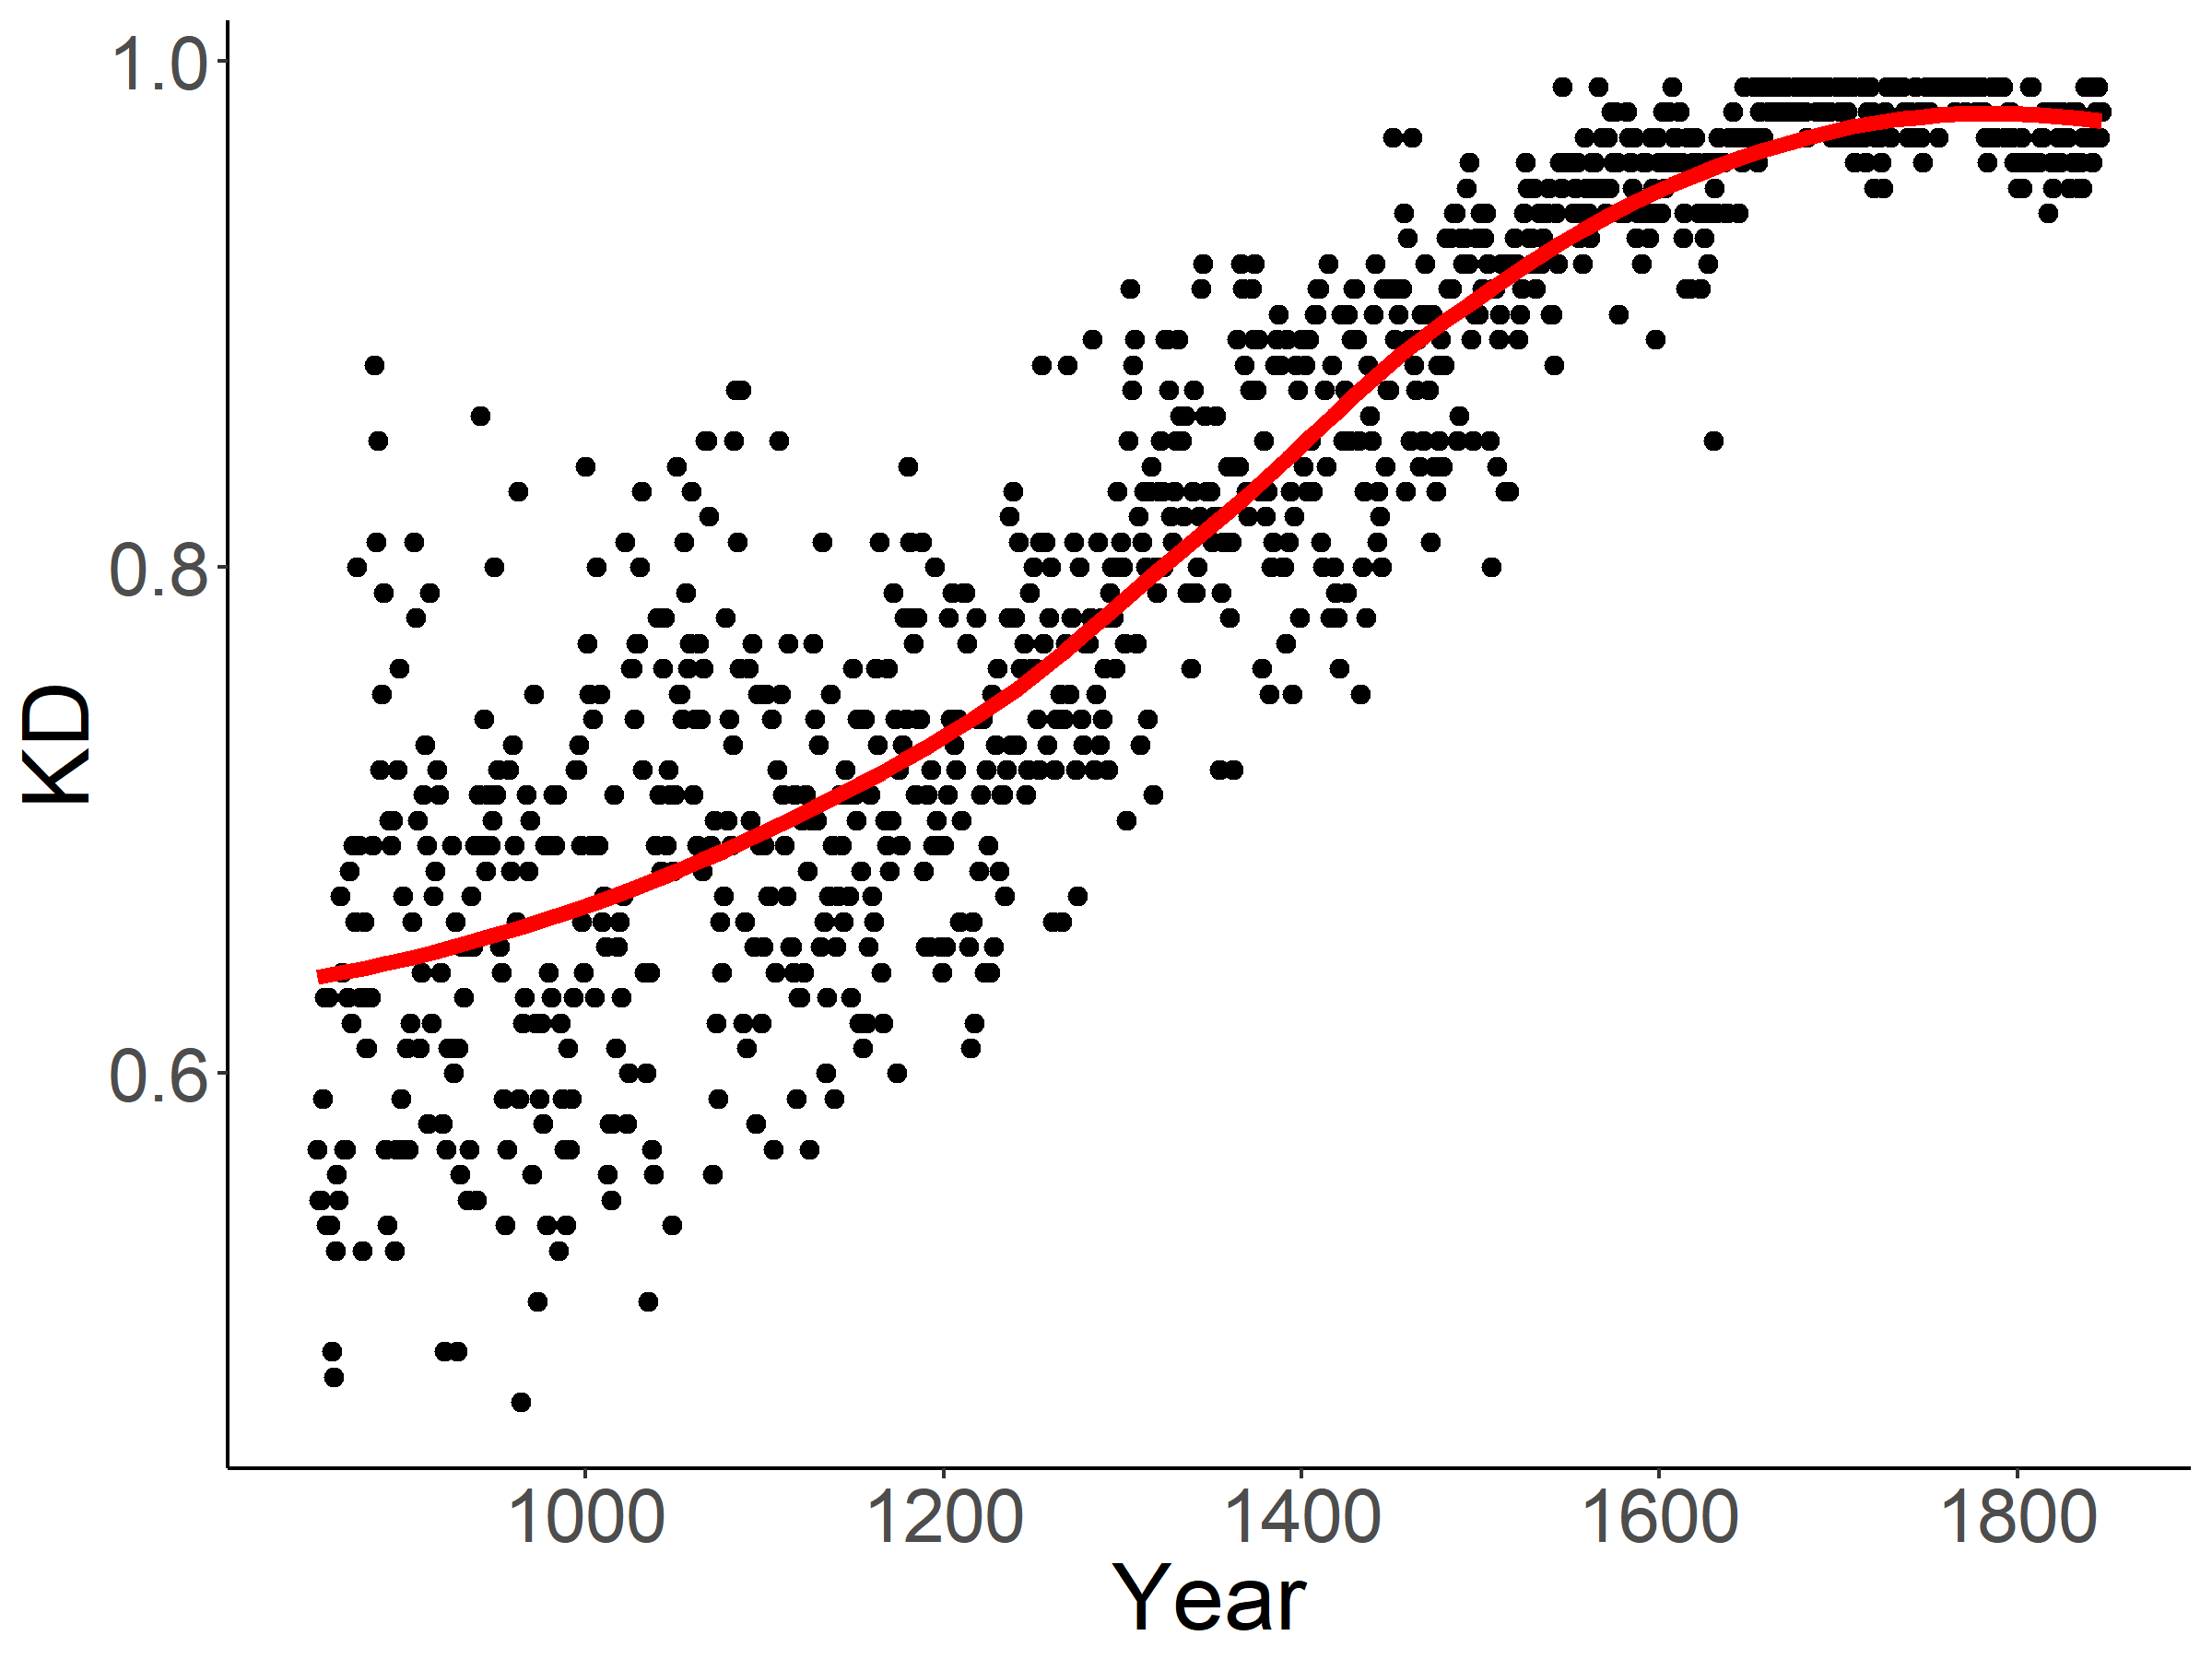
\includegraphics[width=0.45\textwidth]{results/effect_over_time.png}
  }
  \caption{Value of $K$ (left) and associated p-values (right) over the reconstruction years 850 CE to 1850 CE. Larger values of $K$ indicate large differences in distribution.}
  \label{global_results}
\end{figure}

Figure \ref{global_results} shows the magnitude of $K$ over time along with the associated p-values. The p values were adjusted by the Benjamini-Hochberg procedure to have a false discovery rate of 0.05. We interpret their near uniformity about zero as a strong indication that the background and analysis are different in distribution each year. Consequently we believe that the proxies are indeed changing the distribution of the background and hence having a material influence over the assimilation reconstructions.

The magnitudes of $K$ indicate an initial moderate separation between the background and analysis that steadily increases over time until the end of the reconstruction period. The apparent rise in separation is explained by the fact that proxy information is also steadily introduced into the model over time. As the reconstruction nears present day more proxies become available for assimilation and consequently the data assimilation fields should diverge further from the background.

% \begin{figure}
% 	\begin{center}
%     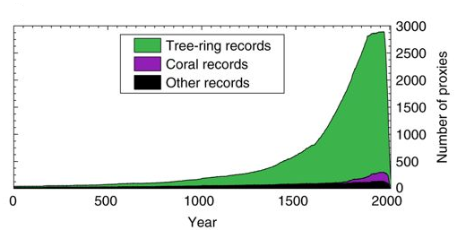
\includegraphics[width=0.50\textwidth,valign=c]{misc/proxytime.png}
%     \caption{Count of proxies used in the reconstructions over time. The sharp uptick in proxies around 1600 CE corresponds to a sharp uptick in $K$.}
%     \label{proxytrend}
%     \end{center}
% \end{figure}

% increasing over time up until the present when the maximum divergence (1.0) is attained. This is the first rigorous confirmation of a long standing belief that increasing the amount of proxy information should increase the amount of separation between the background and analysis states. The PHYDA datasets utilizes a network of over 3000 proxies which are progressively updated into the model as they become temporally available.

% Further we can see that the magnitude of their effect on the distribution is steadily increasing over time. This is to be expected since more proxy information is available and included in more recent years \citet{steiger2018PHYDA}. 

% Next we look at several example years (852, 1150, 1450, 1848) in the data to see how the increasing separation between $F$ and $G_t$ manifests itself as warming or cooling over the background. Using the integrated depth $XD$, defined in section 2.1, we constructed $95\%$ central regions (CR) on the background. The $95\%$ central region estimates the region where the most central, as defined by XD, $95\%$ of the functions sampled from $F$ should fall. Interpreted another way the $95\%$ CR indicates the typical behavior of an arbitrary background field so any values outside of this region would be considered atypical for the background state. Using the background's $95\%$ central region we can visualize the strongest differences between the background and analysis by plotting the average exceedence of the analysis ensemble over (or under) the central region. Locations where the analysis ensemble exceeds the background ensemble's CR on average are warmer or cooler than the vast majority of the background fields at that location. 

% In Figure 7 we show how far on average the analysis ensembles at times 2, 300, 600, and 998 exceed the background's $95\%$ CR.  We can see that the identified regions are highly contiguous but are not consistent in their placement. While the $K$ statistic developed in section 2 is not directly related to these exceedence plots we can see how a larger $K$ tends to correspond with a greater exceedence of the analysis states over the background. However, they should not be interpreted as regions of significant warming or cooling but as guides to the locations of the biggest differences or proxy influence. 

% \begin{figure}
%   \centering
%   \subfloat{%
%     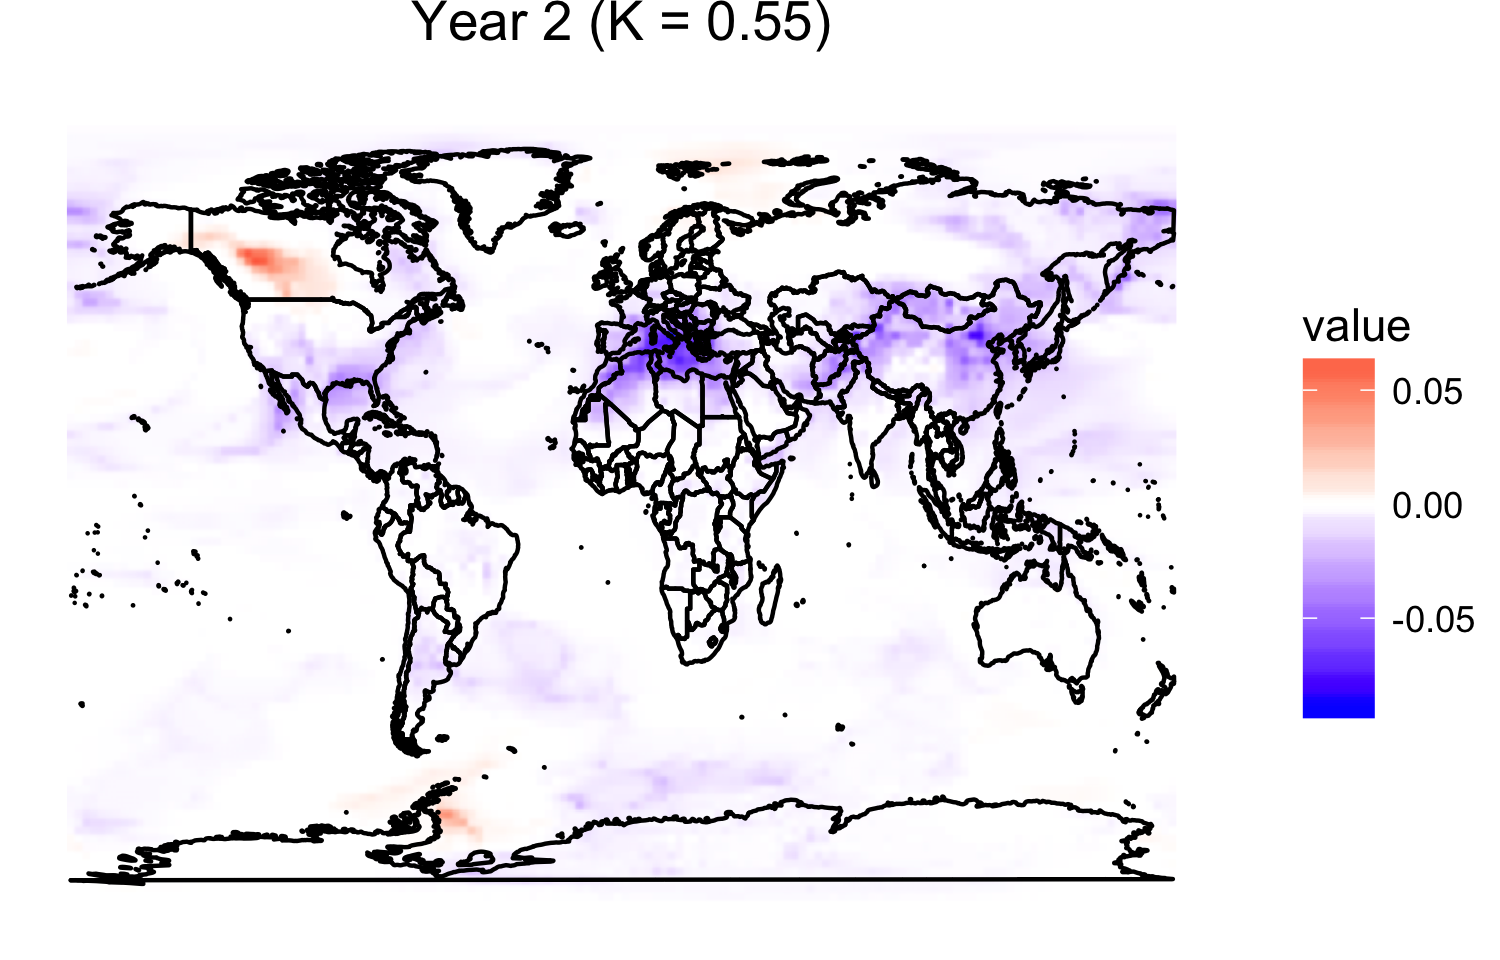
\includegraphics[width=0.45\textwidth]{results/year2field.png}%
%   }
%   \subfloat{%
%     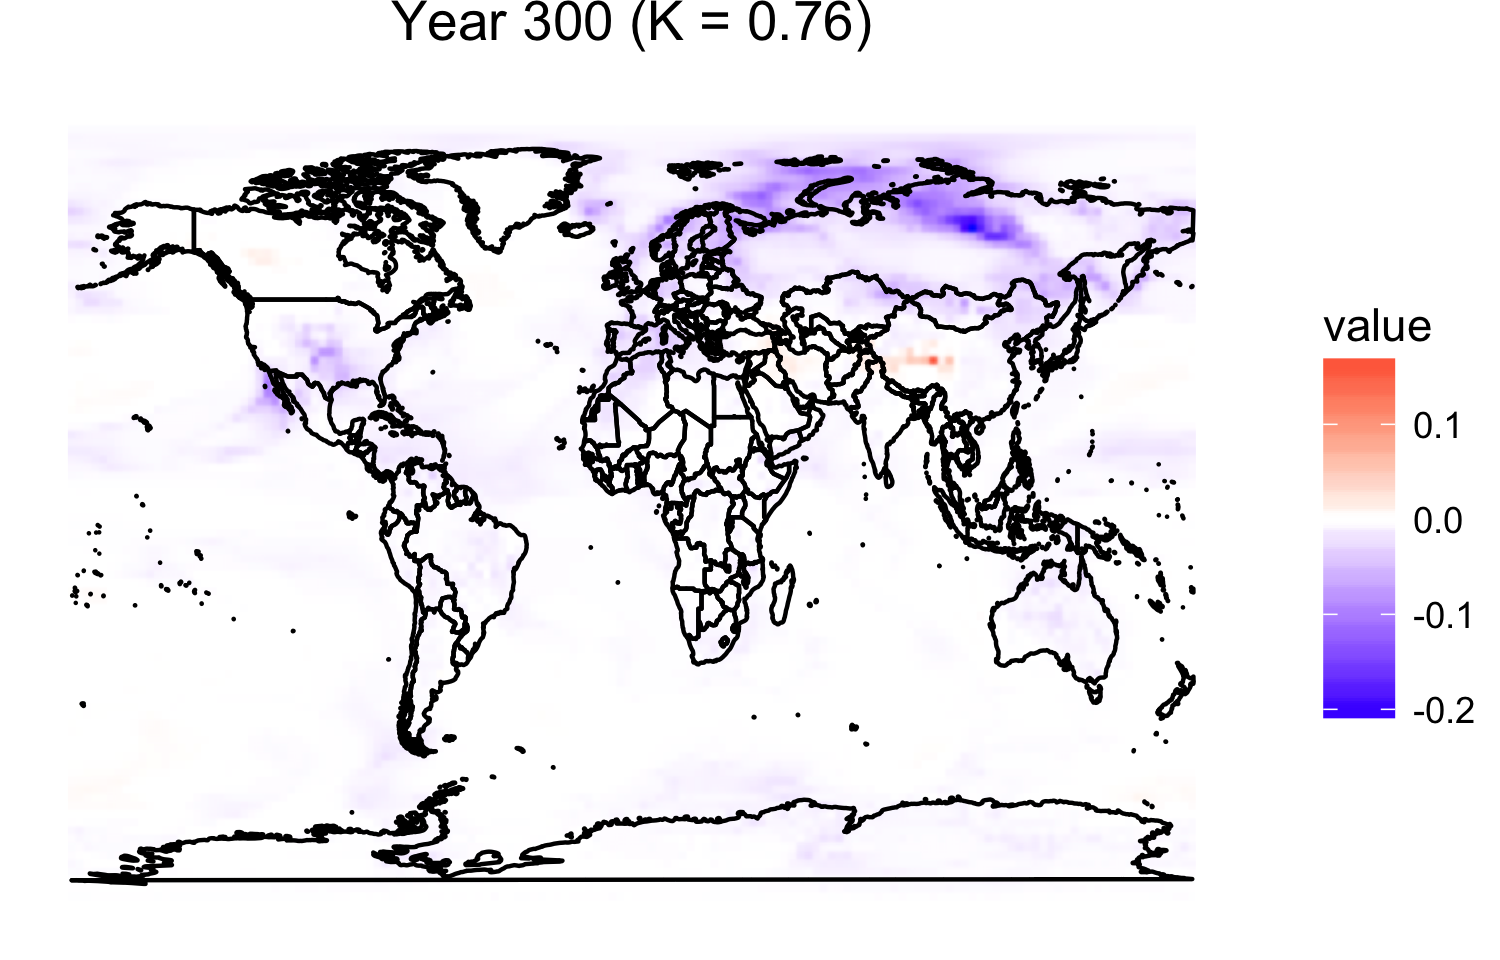
\includegraphics[width=0.45\textwidth]{results/year300field.png}%
%   } \\
%   \subfloat{%
%     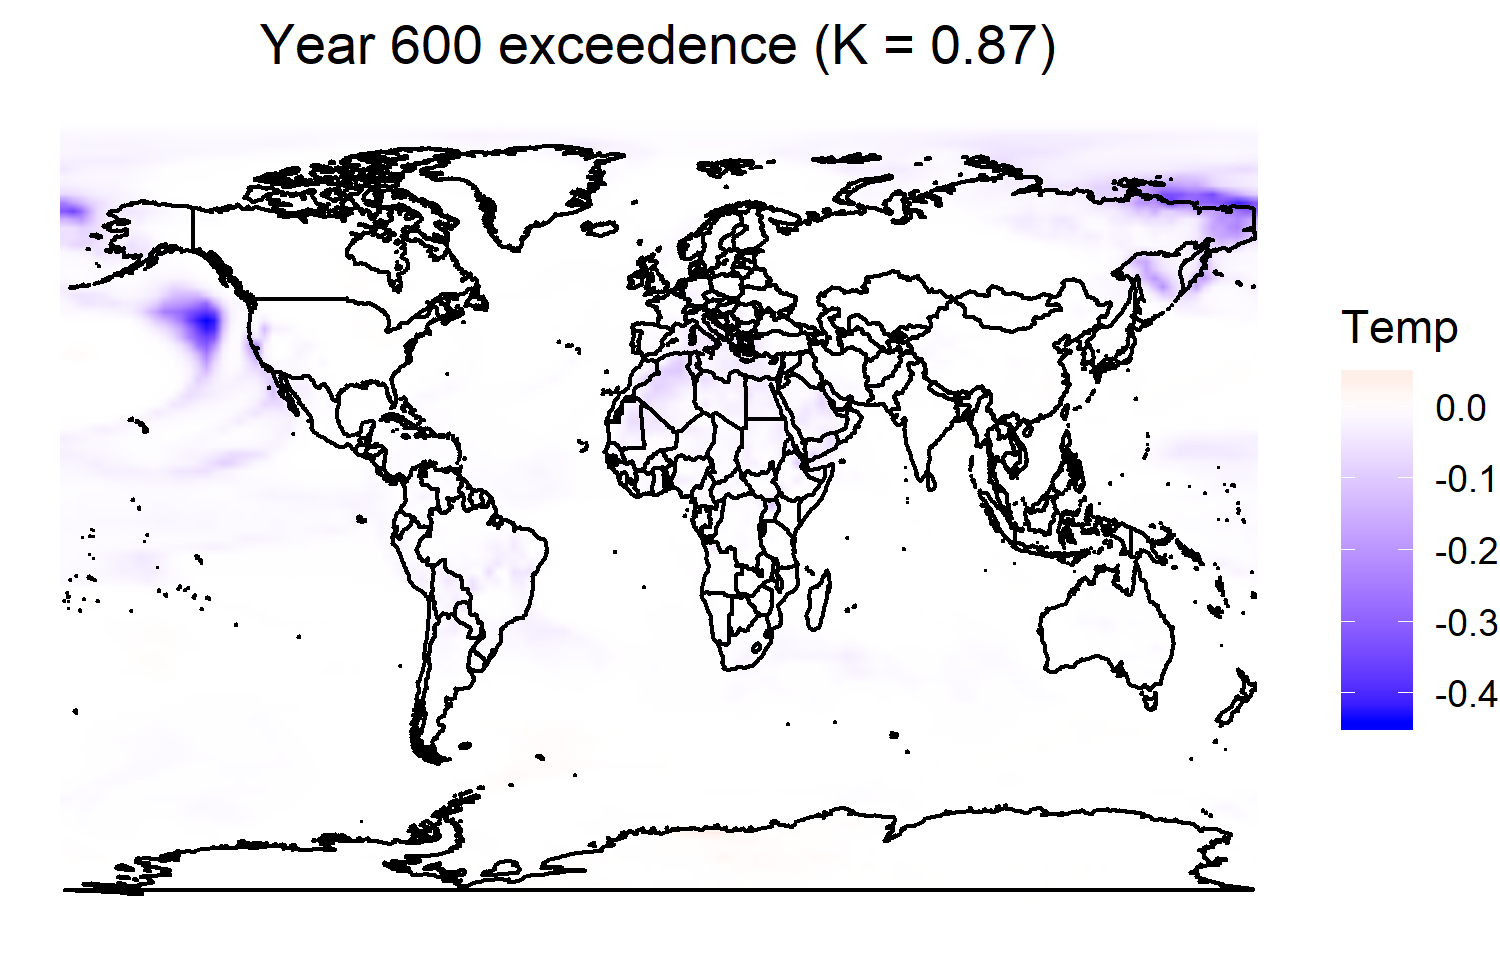
\includegraphics[width=0.45\textwidth]{results/year600field.png}%
%   }
%   \subfloat{%
%     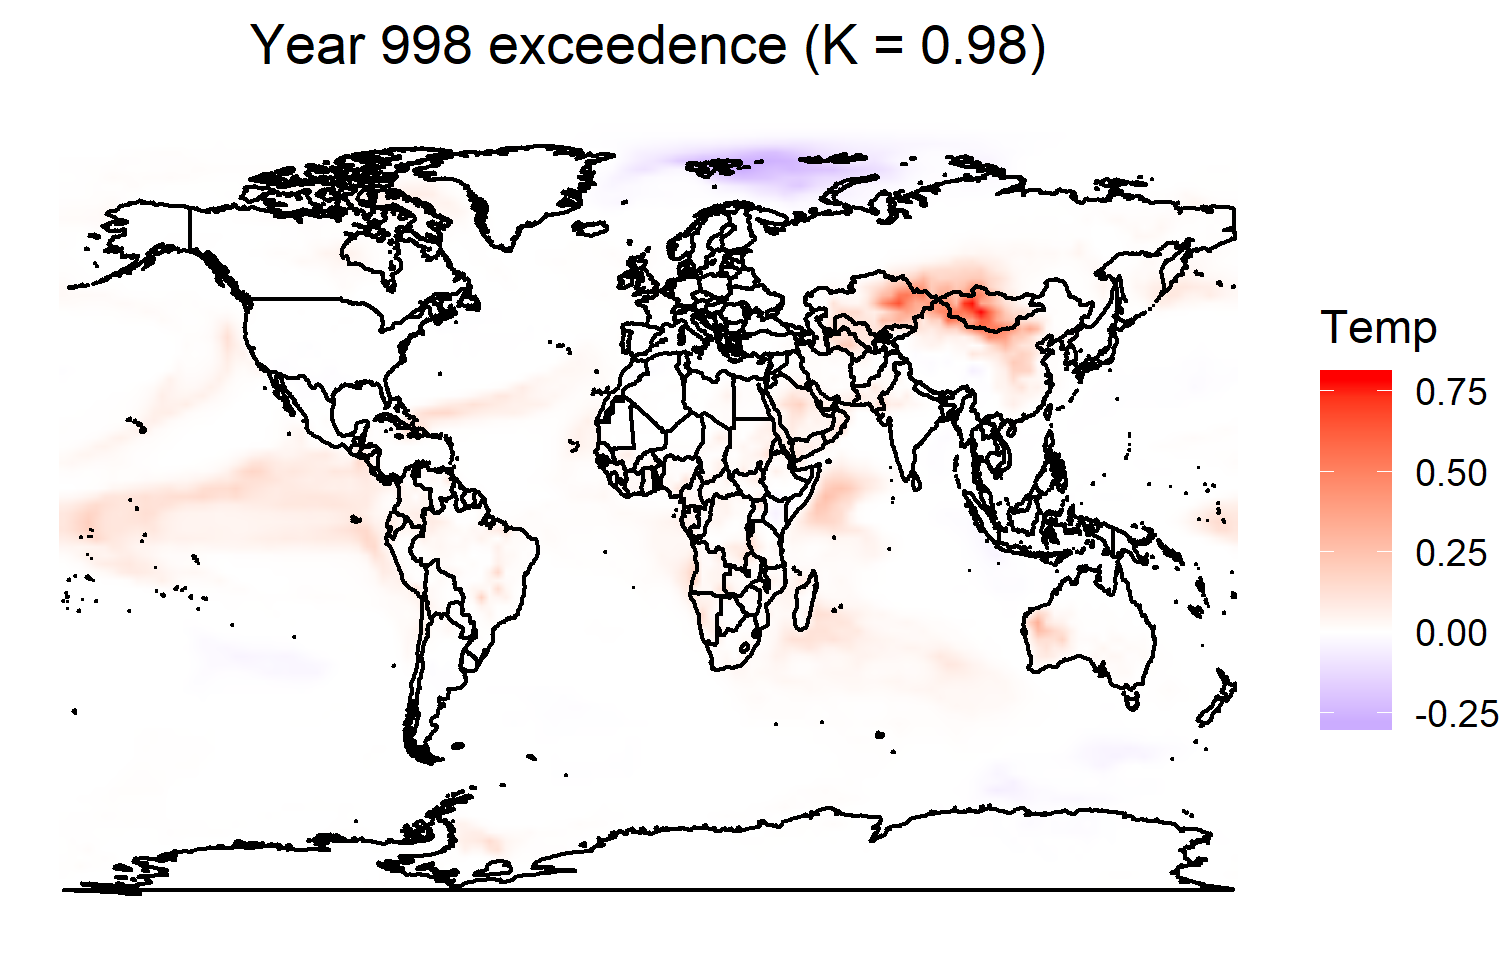
\includegraphics[width=0.45\textwidth]{results/year998field.png}%
%   }
%   \caption{Regions of large deviations between the background and analysis}
% \end{figure}

% \begin{figure}
% 	\begin{center}
%     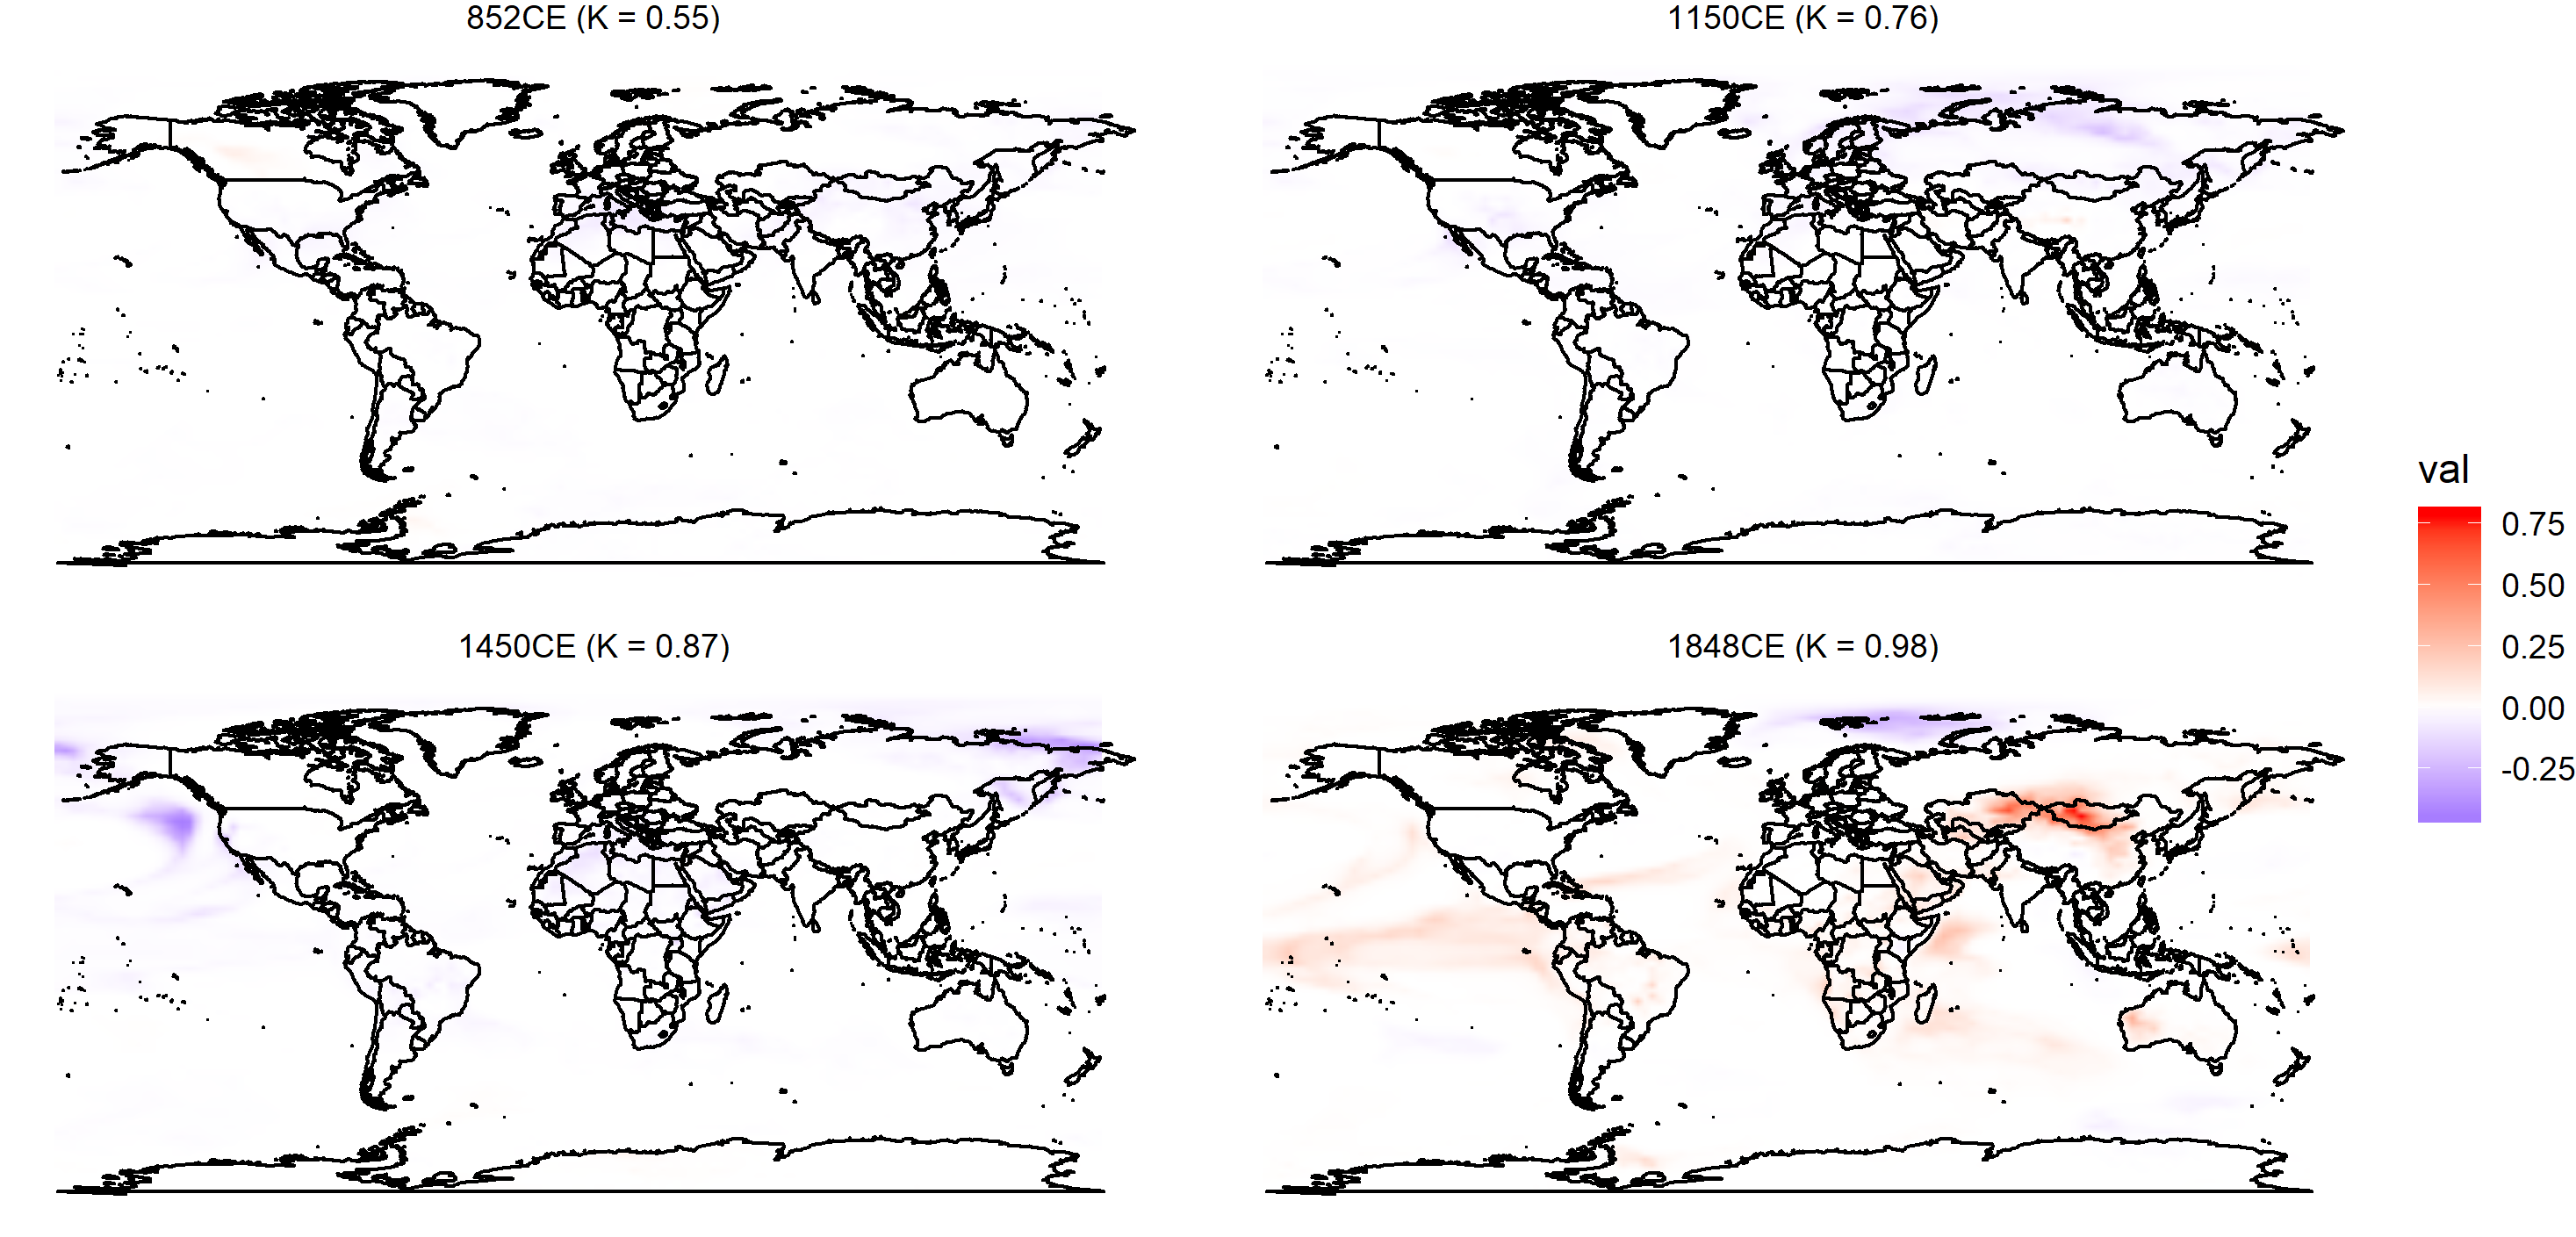
\includegraphics[width=0.90\textwidth,valign=c]{results/multiyear_fields.png}
%     \caption{Regions of large deviations between the background and analysis}
%     \end{center}
% \end{figure}


% Next we wanted to see how patterns of exceedence evolved over time, i.e. how the proxies induced warming or cooling over the baseline. We computed the average $95\%$ CR exceedence of each spatial location at each time in the dataset. In figure 8 the time series of each locations average exceedence has been overlaid to see the aggregate warming or cooling over time. The two most striking features are the strong cooling effect between 650 and 900 (1500--1750 CE) and the sudden reversal to warming following it. The cooling effect is thought to be due to the proxies registering the medieval little ice age more strongly than the GCM alone. This is consistent with the findings in \citet{steiger2014assimilation} based on similar data using the same GCM. The following warming period corresponds to the coinciding end of the ice age and the start of industrialization. By the results of our test we know that these two periods were associated with significant and strong changes in the distribution of the GCM ensemble. We therefore conclude that the proxies are significantly altering the baseline GCM's ability to fully capture centennial scale climate extremes.

% \begin{figure}
% 	\begin{center}
%     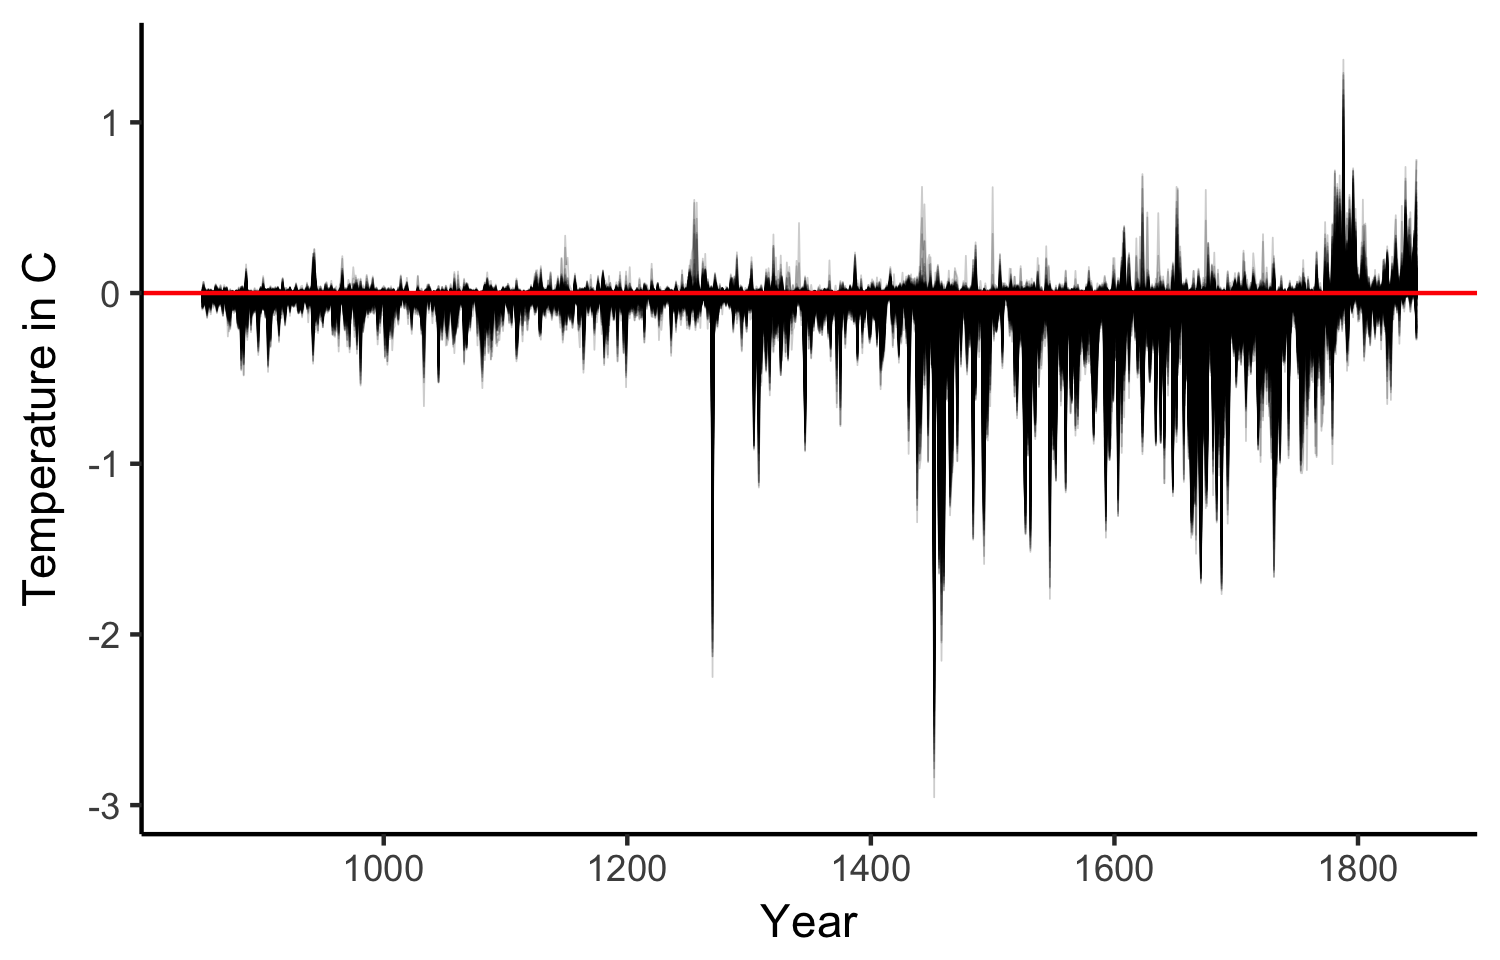
\includegraphics[width=0.60\textwidth,valign=c]{results/trend.png}
%     \caption{Pointwise exceedence trend. Each curve represents the $95\%$ CR exceedence time series for a geospatial location.}
%     \end{center}
% \end{figure}

% \begin{figure}
% 	\begin{center}
%     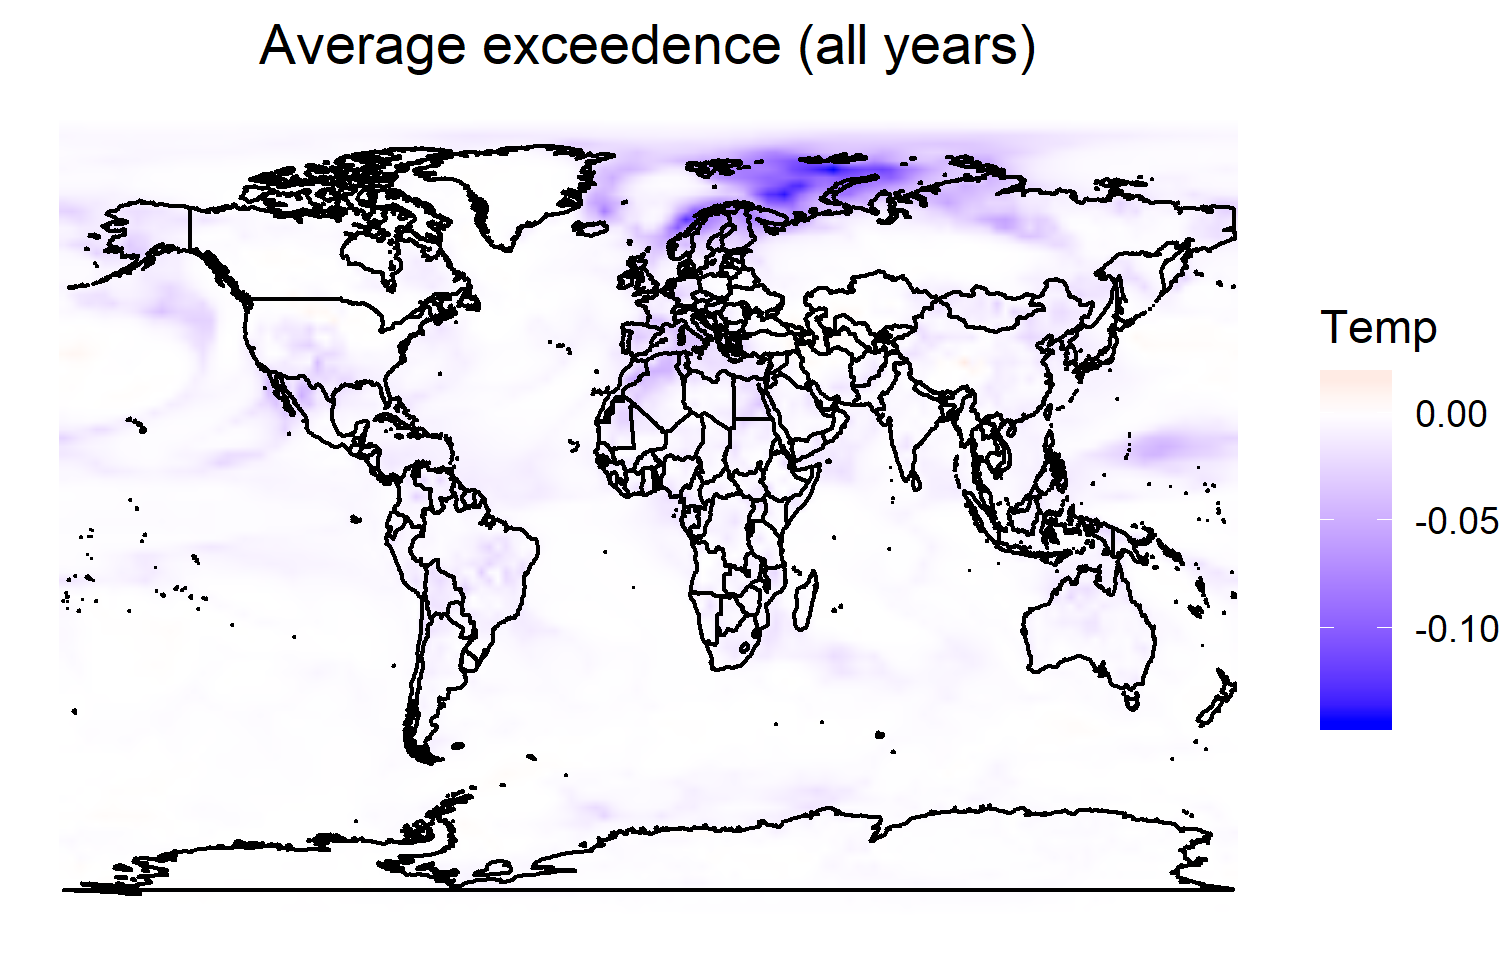
\includegraphics[width=0.60\textwidth,valign=c]{results/average.png}
%     \caption{Average exceedence}
%     \end{center}
% \end{figure}

% In fig. 7. we can see the time series of exceedence for each point in the posterior. A single curve here contains the exceedence of that point over the entire 998 year domain. We can see that most curves are tightly concentrated about 0 for the first 500 years, i.e. 850 CE to 1350 CE. Between 1350 CE and 1750 CE there is a noticeable cooling effect which is the primary driver of the Fig. 6. We postulate that because of the timing and the regions impacted that this is due to the medieval little ice age. Finally towards the end there is a definite and strong positive exceedence amongst almost all curves, indicating a mild global warming during the time period leading up to 1850 CE. \textcolor{red}{The fact that the proxies picked up on the little ice age and the model did not is interesting right?}

\subsection{Regional Variations} \label{regional}
Analysis of the global fields is important for establishing the strength of proxy influence in the model as a whole and for confirming the existence of its upward trend. A natural next step then is to consider how these effects distribute down to a regional level; namely how proxies impact climatological estimation at the continental and oceanic level. Proxies are not collected uniformly across all regions and there is a clear over representation in North America and Europe and under representation in Africa, South America and large swathes of the oceans, Fig. \ref{regions}. We would thus not expect proxies to have as strong of an effect over these latter regions as we would the former. Still, owing to a long range correlation structure evidenced between surface temperature and the proxies (Fig. \ref{corr}) we believe that these regional deficits may be somewhat mitigated. Our results provide a measure of support for this hypothesis since we see strong divergence between the background and analysis in Africa and the Pacific.

\begin{figure}
  \centering
  \subfloat{%
    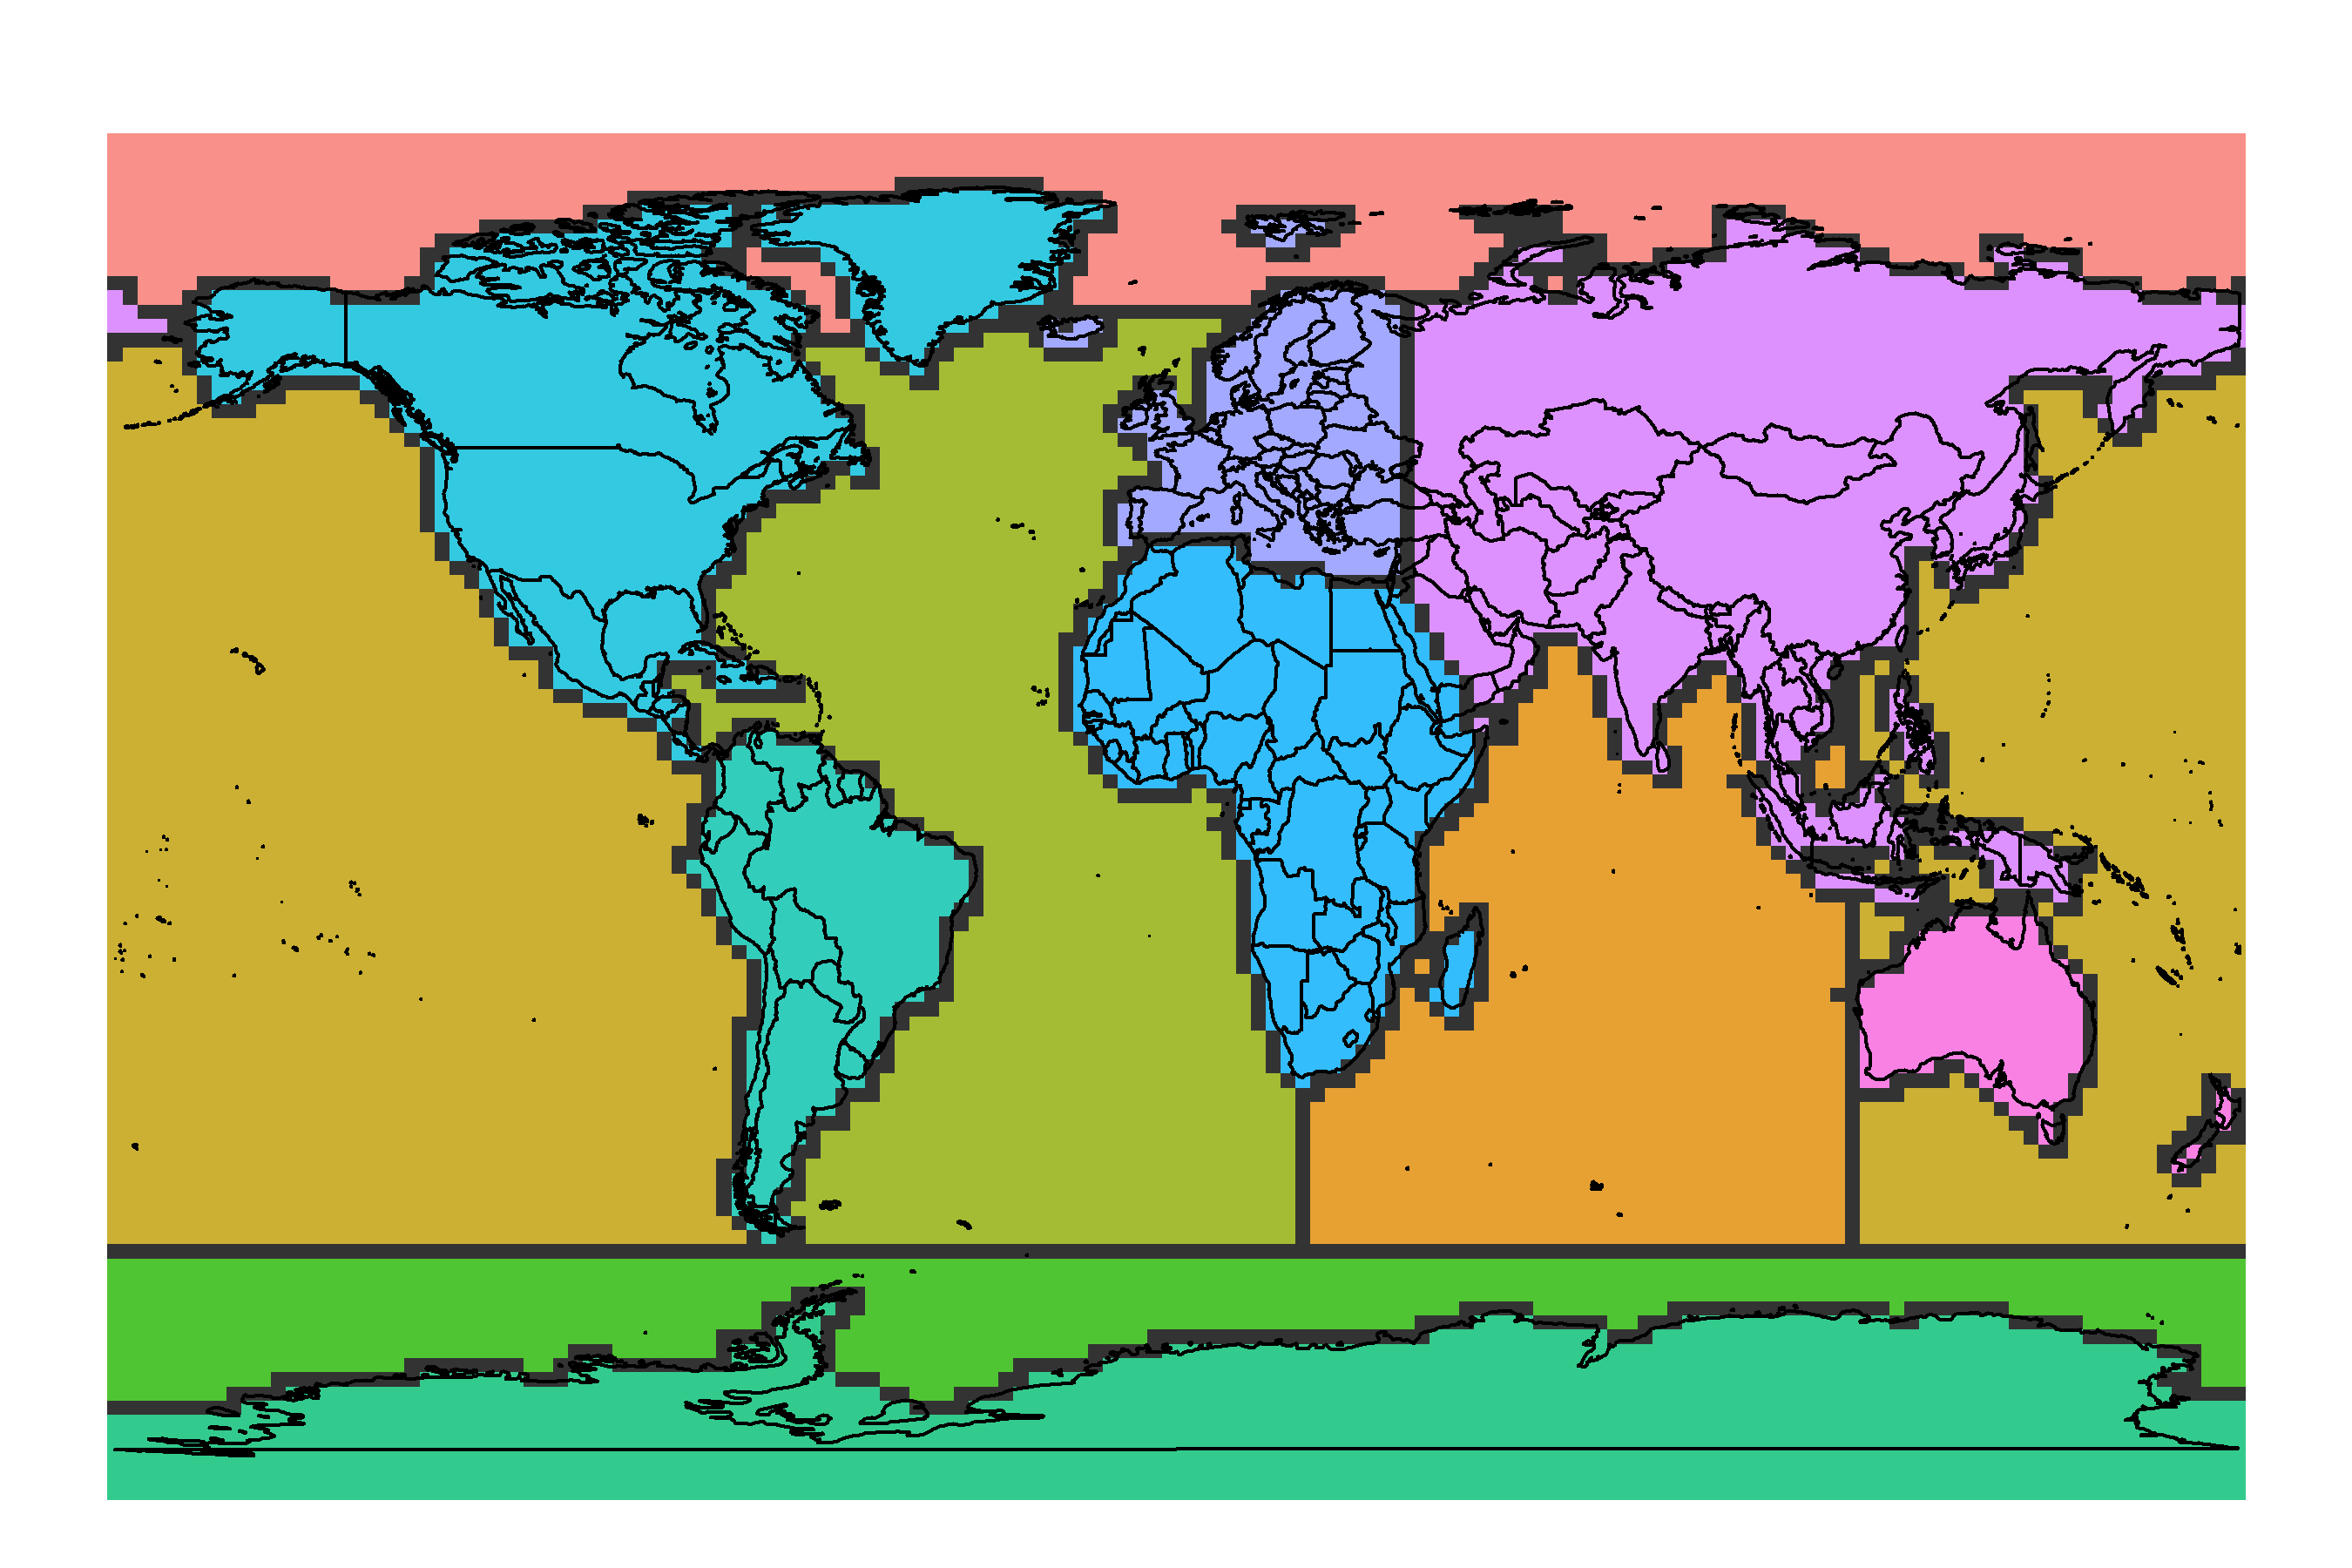
\includegraphics[width=0.4\textwidth]{misc/regions.png}
  }
  \subfloat{%
    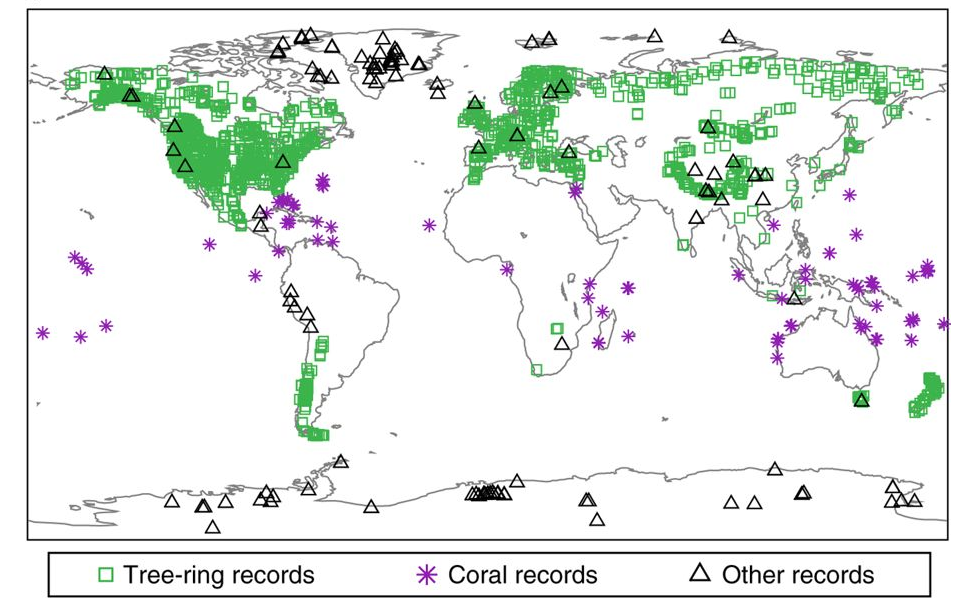
\includegraphics[width=0.4\textwidth]{misc/proxies.png}
  }
  \caption{Regions versus proxy locations. The vast majority of proxies are collected in convenient locations such as North America and Europe. Not all of the displayed proxies are available every year in the reconstruction, as reconstruction gets closer to the present day more become available.}
  \label{regions}
\end{figure}

We split the global background and analysis ensembles into 12 regions corresponding to the five oceans and seven continents, Fig. \ref{regions}. Within each of the twelve regions we used our $K$ statistic to test for differences in the background and analysis states over the full reconstruction period. 
\begin{figure}
	\begin{center}
    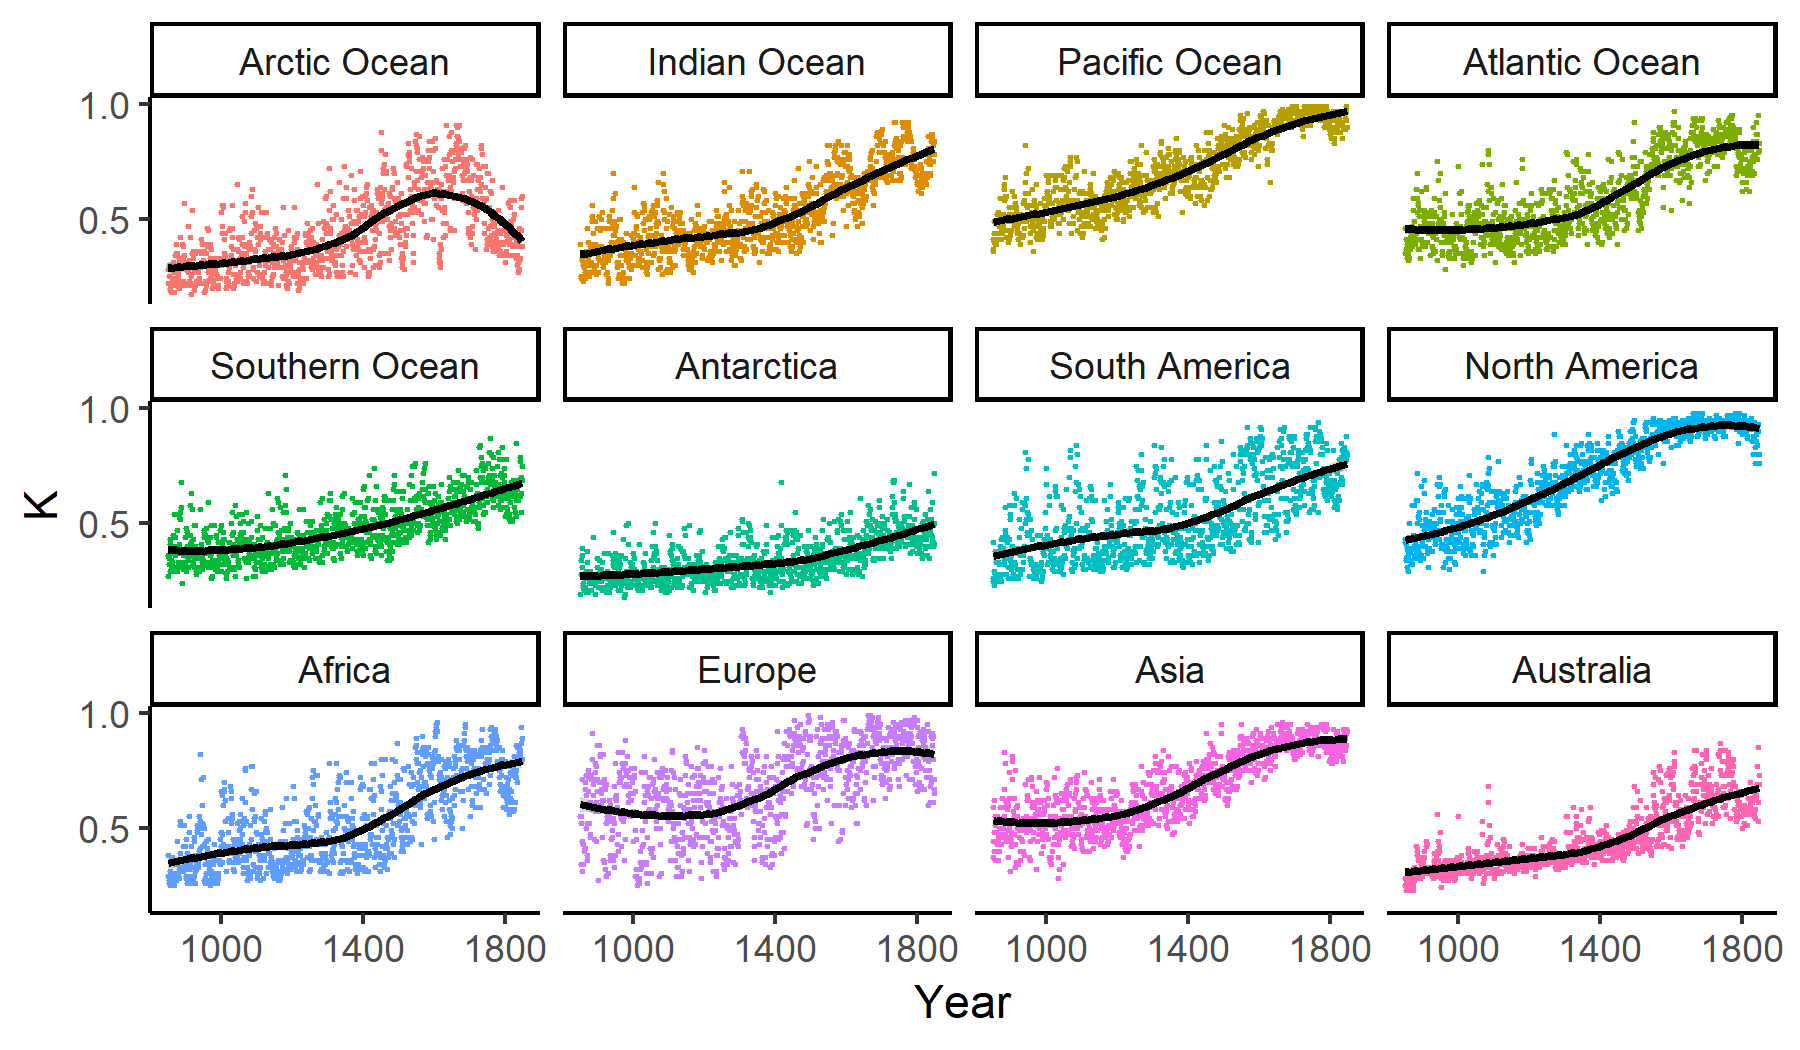
\includegraphics[width=0.80\textwidth,valign=c]{results/k_region.png}
    \caption{K over time by region. Regional K values were computed by only measuring differences in the region of interest within the Global reconstructions. They generally follow the pattern of the Global K values with the exception of the Arctic Ocean.}
    \label{kregion}
    \end{center}
\end{figure}
Our findings are summarized in Figure \ref{kregion} and supported by Figures \ref{corr} and \ref{pvalregion}. Figure \ref{kregion} shows $K$'s progression over time for each region, analogous to the global study in Fig. \ref{global}. The increasing effect size over time in each region is determined most strongly by the increasing proxy information availability in time. As proxy information is gradually introduced over time the analysis states becomes more and more distinct from the background. This effect holds true even for some regions where proxy information is relatively scarce. However, because the strength of the climatological connections between various regions are different from one another, the proxy information will not be uniformly dispersed and so not all regions will benefit equally. Therefore it can be helpful to consider the spatial extent over which proxies in different locations can have an influence on the analysis state. This can be estimated by looking at proxy-point correlation maps at different points in time, Fig. \ref{corr}. A thorough explanation of how these maps are created can be found in the appendix.

\begin{figure}
	\begin{center}
    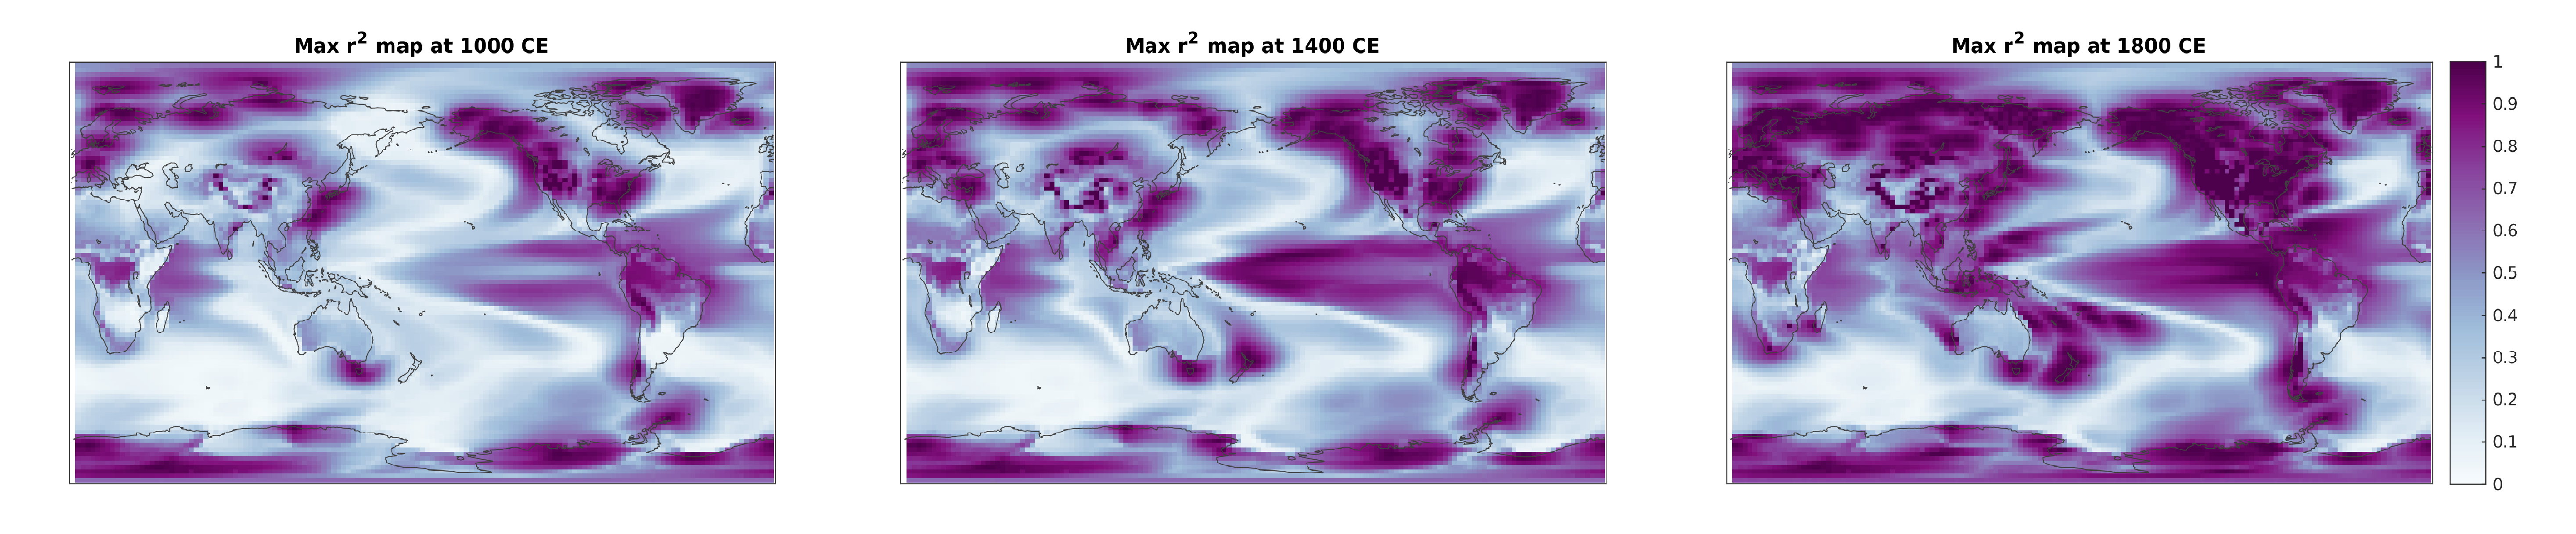
\includegraphics[width=\textwidth,valign=c]{misc/corr_map.png}
    \caption{Proxy-point correlation maps for representative years 1000, 1400, and 1850 CE. There is an overall increasing proxy point correlation (purple) in time. This is reflected in the increasing effect sizes seen in regions with little proxy representation.}
    \label{corr}
    \end{center}
\end{figure}

The maximum $r^2$ values decrease further back in time as fewer proxies are available. The spatial extent of the correlations thus provide a guide to interpreting the  general decrease in effect size as well as the differences in the effect size between regions. Regions with higher max $r^2$ values generally have higher effect sizes (e.g., comparing North America with Australia). Note that some regions (particularly the Pacific ocean) can have few proxies but are highly correlated with other regions of the globe that have many proxies (seen in the larger max $r^2$ values in Fig. \ref{corr}), therefore their effect sizes can remain high despite the lack of local proxies. 

The Arctic and Southern oceans represent two anomalies with regards to their supposed proxy information. Most noticeably around 1600 the Arctic ocean experiences a strong trend reversal in $K$, just when other regions are experiencing trend increases. This runs counter to the fact that number proxies and the proxy-point correlation are both increasing in the Arctic over this time period. Conversely the Southern ocean has relatively large values of $K$ when proxy information would lead us to believe they should be much smaller. The Southern ocean has no collected proxies and it has some of the weakest overall proxy-point correlation strength, yet it experiences a strong and significant divergence between its background and analysis states. It is currently unclear why either the Arctic or Southern ocean are behaving differently than their levels of proxy information would indicate.

% Figure XX is constructed by first computing point correlation maps for the prior 2 m temperature time series for each proxy location: the prior is a continuous climate model simulation and the correlation is computed between the 2 m temperature time series at a given proxy location and all global grid point 2 m temperature time series in the prior. This generates nearly 3,000 correlation maps, one for each proxy location. Then for the representative years of 1000, 1400, and 1800 CE, the maximum $r^2$ value is found for each grid point among all the correlation maps that correspond to the proxies that are available during those specific years. 

\begin{figure}
	\begin{center}
    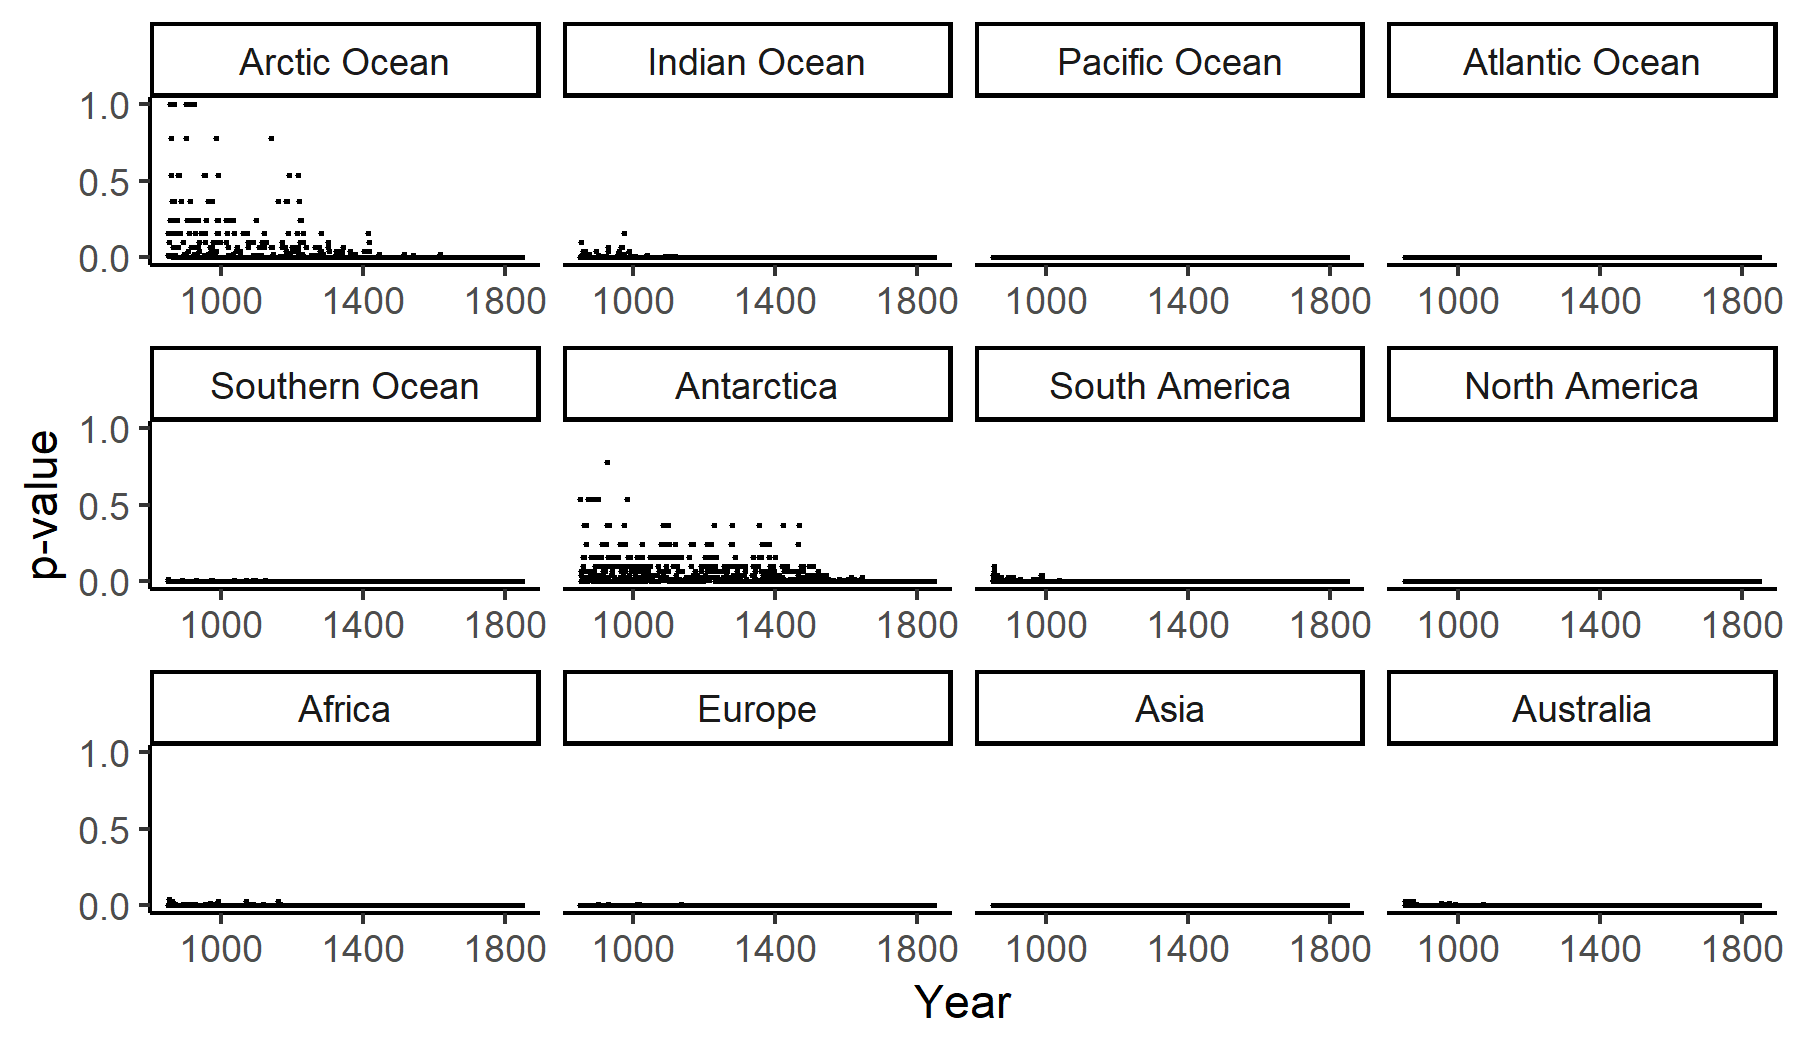
\includegraphics[width=0.80\textwidth,valign=c]{results/pval_region.png}
    \caption{P-values of K over time by region}
    \label{pvalregion}
    \end{center}
\end{figure}

% \begin{figure}
% 	\begin{center}
%     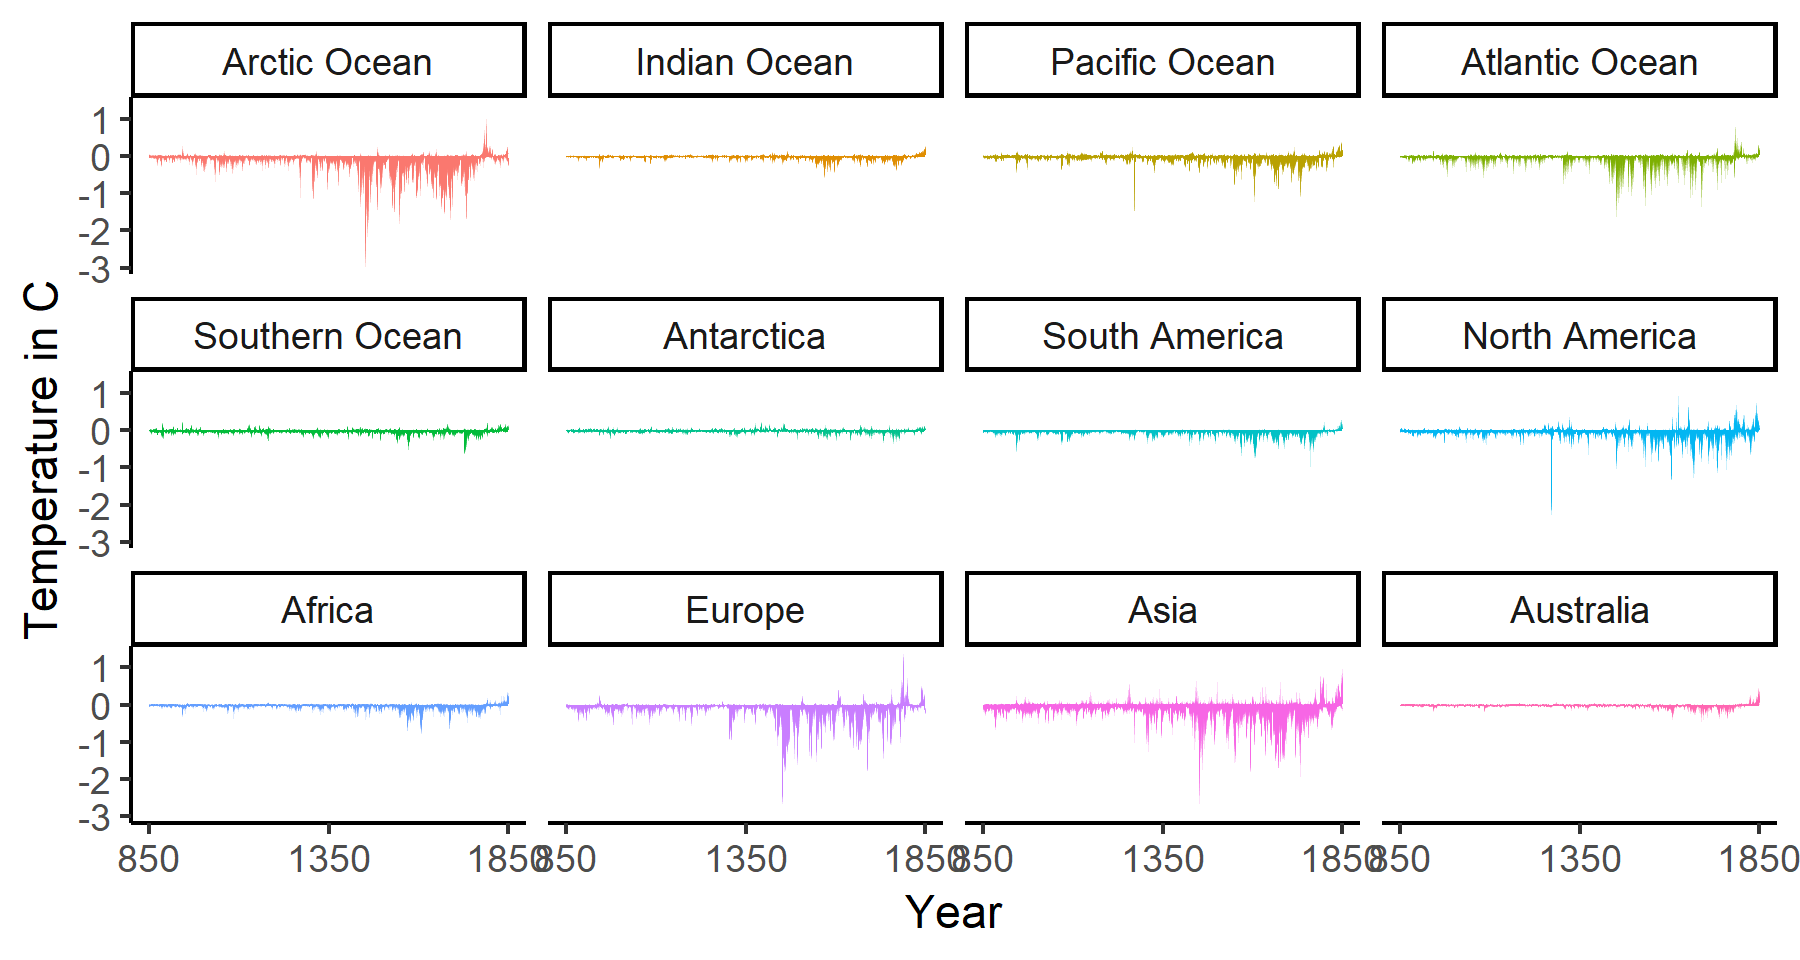
\includegraphics[width=0.80\textwidth,valign=c]{results/regional_exceedence.png}
%     \caption{Pointwise exceedence trend. Each curve represents the $95\%$ CR exceedence time series for a geospatial location.}
%     \end{center}
% \end{figure}

\section{Discussion} \label{discussion}
By estimating differences in the background and analysis's distributions we were able to investigate the influence proxies hold over the data assimilation process. Our investigation centered on studying the existence and degree of influence, how influence develops over time, and how influence is distributed spatially. Existing two sample functional data tests were found to be insufficient for answering these questions due to both testing and data limitations. Most tests only consider specific quantities such as mean differences which do not represent the full role that proxies can play. Of those that do consider distributional differences they either rely on bootstrapping (hall) and are thus too slow for data of this size or they utilize basis representations (strecu) which struggle to capture the subtle variations proxies induce. To overcome these limitations we developed a new non-parametric two sample test for functional distributions. This test was seen to control the size well, even with small sample sizes, and to be powerful against changes in location, scale, and correlation structure. Its foundation in a computationally efficient data depth function means that it is also fast enough to evaluate on large climate data sets, such as considered here.

Our results on the global reconstructions provide strong evidence of a clear separation between the background and analysis, but that the degree of separation depends heavily on reconstruction location and period. There was seen to be overall upward trend in proxy influence which is generally maintained even when subdividing the data into oceanic and continental sub-regions. With the notable exception of the Arctic, these findings are consistent with the fact that proxy information steadily increases as the reconstruction period approaches the present day. This is the first rigorous confirmation of the long standing, educated, belief that increasing proxy information should correlate with a commensurate increase in separation.

It was also seen that, despite the stark imbalance in proxy density across the various regions, most regions still exhibited an increasing separation. This mitigating effect is mostly attributable to the long range correlation structure proxies and temperatures often display. Some regions such as Pacific and South America have very few local proxies but due to their significant correlation with other regions still benefit from proxies collected remotely.

Looking forward, our results indicate that as more proxy data is collected and assimilated climate models will increasingly reflect the climatic states of past Earth. This has far reaching consequences for those who use long run paleoclimate reconstructions to inform predictions about future climate. Furthermore the two sample test developed here is much more broadly applicable than for studying proxy influence. Our generic formulation allows it to be applied seamlessly on any functional data that the depth function can handle, including curves in $\mathbbm{R}$ and higher dimensional functions in $\mathbbm{R}^n$. We hope that future work can both establish our tests asymptotic distribution and study its efficacy in higher dimensions.

Also, because our test is based on integrated depth and not distances or principal components the assumptions we need to make about the data are very light. We do not need to assume that the curves are square integrable, second order stationary, densely sampled, or even strictly continuous. Computing the integrated Tukey depth merely requires that the functions are almost everywhere continuous and observed at the same locations. The first requirement allows us to consider discrete or continuous functions without any modification to the procedure. The second is typically not an issue for densely sampled data since it can be interpolated onto a shared grid with little loss in accuracy. The assumptions that $P$ and $Q$ are absolutely continuous distributions and that each $X_i$ and $Y_j$ is univariate could also be relaxed. Letting $P$ and $Q$ be discrete distributions simply changes the measure used for integration to the counting measure. Each $X_i$ and $Y_j$ could also be multivariate valued so long as they both map to the same subspace of $\mathbbm{R}^p$. This only changes our integration to be over a multivariate depth instead of a univariate depth. We did not explore or test these generalized settings in this paper but we make note of them to highlight the flexibility allowed for by depth based testing.


% Because the PHYDA reconstruction design does not propagate information forward in time we were able to isolate proxy influence down to differences in background and analysis's distributions. 

% In summary we have developed a new non-parametric two-sample test for testing if two functional distributions are equal and derived its asymptotic distribution. Our test is based on the concept of integrated functional data depth which makes it highly efficient and completely distribution free. We used it to study the influence of proxies in data assimilation algorithms by treating the GCM estimates (background) and the data assimilation estimates (analysis) as samples of random continuous surfaces. Our results show that the inclusion of proxies significantly alters the distribution of the GCM estimates and but that these differences are not uniform across the globe. We also found that proxies are registering climatic events such as the medieval little ice age and forcing the data assimilation ensembles to reflect them. 

\section*{Acknowledgments}
This paper describes objective technical results and analysis. Any subjective views or opinions that might be expressed in the paper do not necessarily represent the views of the U.S. Department of Energy or the United States Government.
This work was supported by the Laboratory Directed Research and Development program at
Sandia National Laboratories, a multi-mission laboratory managed and
operated by National Technology and Engineering Solutions of Sandia,
LLC, a wholly owned subsidiary of Honeywell International, Inc., for the
U.S. Department of Energy's National Nuclear Security Administration
under contract DE-NA0003525.
Working datasets were provided by Jason Smerdon and Nathan Steiger of the Lamont-Doherty Earth Observatory (LDEO) at Columbia University.

\appendix
\section{Appendix}

\subsection{Proofs}

\textbf{Proposition \ref{asymptotic}}
% \begin{proposition}
% Suppose that $n \gg m$, then 
% \[
% K_{P_n}(P, Q) = \sqrt{\frac{nm}{n+m}} \max_{x \in X}|\widehat{F}_n(x) - \widehat{G}_m(x)|
% \]
% converges in law to the Kolmogorov Distribution under the null hypothesis.
% \end{proposition}

% \begin{proof}
% \begin{align*}
%     \sqrt{\frac{nm}{n+m}} \max_{x \in X}|\widehat{F}_n(x) - \widehat{G}_m(x)| &= \sqrt{m} \max_{x \in X}|\widehat{F}_n(x) - \widehat{G}_m(x)| \\
%     &= \sqrt{m} \max_{x \in X}|F(x) - \widehat{G}_m(x)| \\
%     &= \sqrt{m} \max_{x \in X}|G(x) - \widehat{G}_m(x)|
% \end{align*}
% \end{proof}

\begin{proof}
let $P$ be a distribution on $C[0, 1]^p$ and suppose $X = \{X_1,...,X_n\}$ and $Y = \{Y_1,...,Y_n\}$ are two i.i.d samples from $P$. Let $\widehat{F}_n(\cdot)$ and $\widehat{G}_m(\cdot)$ be defined as before with each converging in distribution to $F$, the distribution over $D(\cdot, P)$. Let $x \in X$, then
\begin{align*}
    &\quad \sqrt{\frac{nm}{n+m}} \max_{x \in X}|\widehat{F}_n(x) - \widehat{G}_m(x)| \\
    &\leq \sqrt{\frac{nm}{n+m}} \max_{x \in X}|\widehat{F}_n(x) - F(x)| +  \sqrt{\frac{nm}{n+m}} \max_{x \in X}| F(x) - \widehat{G}_m(x)| \\
    &\simeq \sqrt{m} \max_{x \in X}|\widehat{F}_n(x) - F(x)| +  \sqrt{m} \max_{x \in X}| F(x) - \widehat{G}_m(x)|,
\end{align*}
Since $n \gg m$. By the enforced uniformity of $\widehat{F}_n(x)$ we get that $\max_{x \in X}|\widehat{F}_n(x) - F(x)| = o_p(\frac{1}{\sqrt{n}})$ and so the following upper bound
\begin{align*}
    &\leq o_p(1) +  \sqrt{m} \max_{x \in X}| F(x) - \widehat{G}_m(x)|
\end{align*}
The second term is simply a one sample Kolmogorov-Smirnov statistic so the whole quantity converges to the Kolmogorov distribution.
\end{proof}

% \begin{proof}
% Let $F$ be the distribution of $D(x, P)$ for some known $P$ and assuming $x \sim P$. Then  
% \begin{align*}
%     &\quad \sqrt{\frac{nm}{n+m}} \max_{x \in X}|\widehat{F}_n(x) - \widehat{G}_m(x)| \\
%     &\leq \sqrt{\frac{nm}{n+m}} \max_{x \in X}|\widehat{F}_n(x) - F(x)| +  \sqrt{\frac{nm}{n+m}} \max_{x \in X}| F(x) - \widehat{G}_m(x)| \\
%     &\simeq \sqrt{m} \max_{x \in X}|\widehat{F}_n(x) - F(x)| +  \sqrt{m} \max_{x \in X}| F(x) - \widehat{G}_m(x)|,
% \end{align*}
% Since $n \gg m$. Using this fact again and that $\max_{x \in X}|\widehat{F}_n(x) - F(x)| = o_p(\frac{1}{\sqrt{n}})$ we get the following upper bound
% \begin{align*}
%     &\leq o_p(1) +  \sqrt{m} \max_{x \in X}| F(x) - \widehat{G}_m(x)| \\
%     &= o_p(1) +  \sqrt{m} \max_{x \in X}| G(x) - \widehat{G}_m(x)|,
% \end{align*}
% under the null hypothesis. The second term is simply a one sample Kolmogorov-Smirnov statistic so the whole quantity converges to the Kolmogorov distribution.
% \end{proof}

\subsection{Correlation Maps}
The correlation maps in figure \ref{corr} are constructed by first computing point correlation maps for the background 2 m temperature time series for each proxy location: the background is a continuous climate model simulation and the correlation is computed between the 2 m temperature time series at a given proxy location and all global grid point 2 m temperature time series in the background. This generates nearly 3,000 correlation maps, one for each proxy location. Then for the representative years of 1000, 1400, and 1800 CE, the maximum $r^2$ value is found for each grid point among all the correlation maps that correspond to the proxies that are available during those specific years.

\subsection{Power Plots}
% \begin{figure}[H]
% 	\begin{center}
%     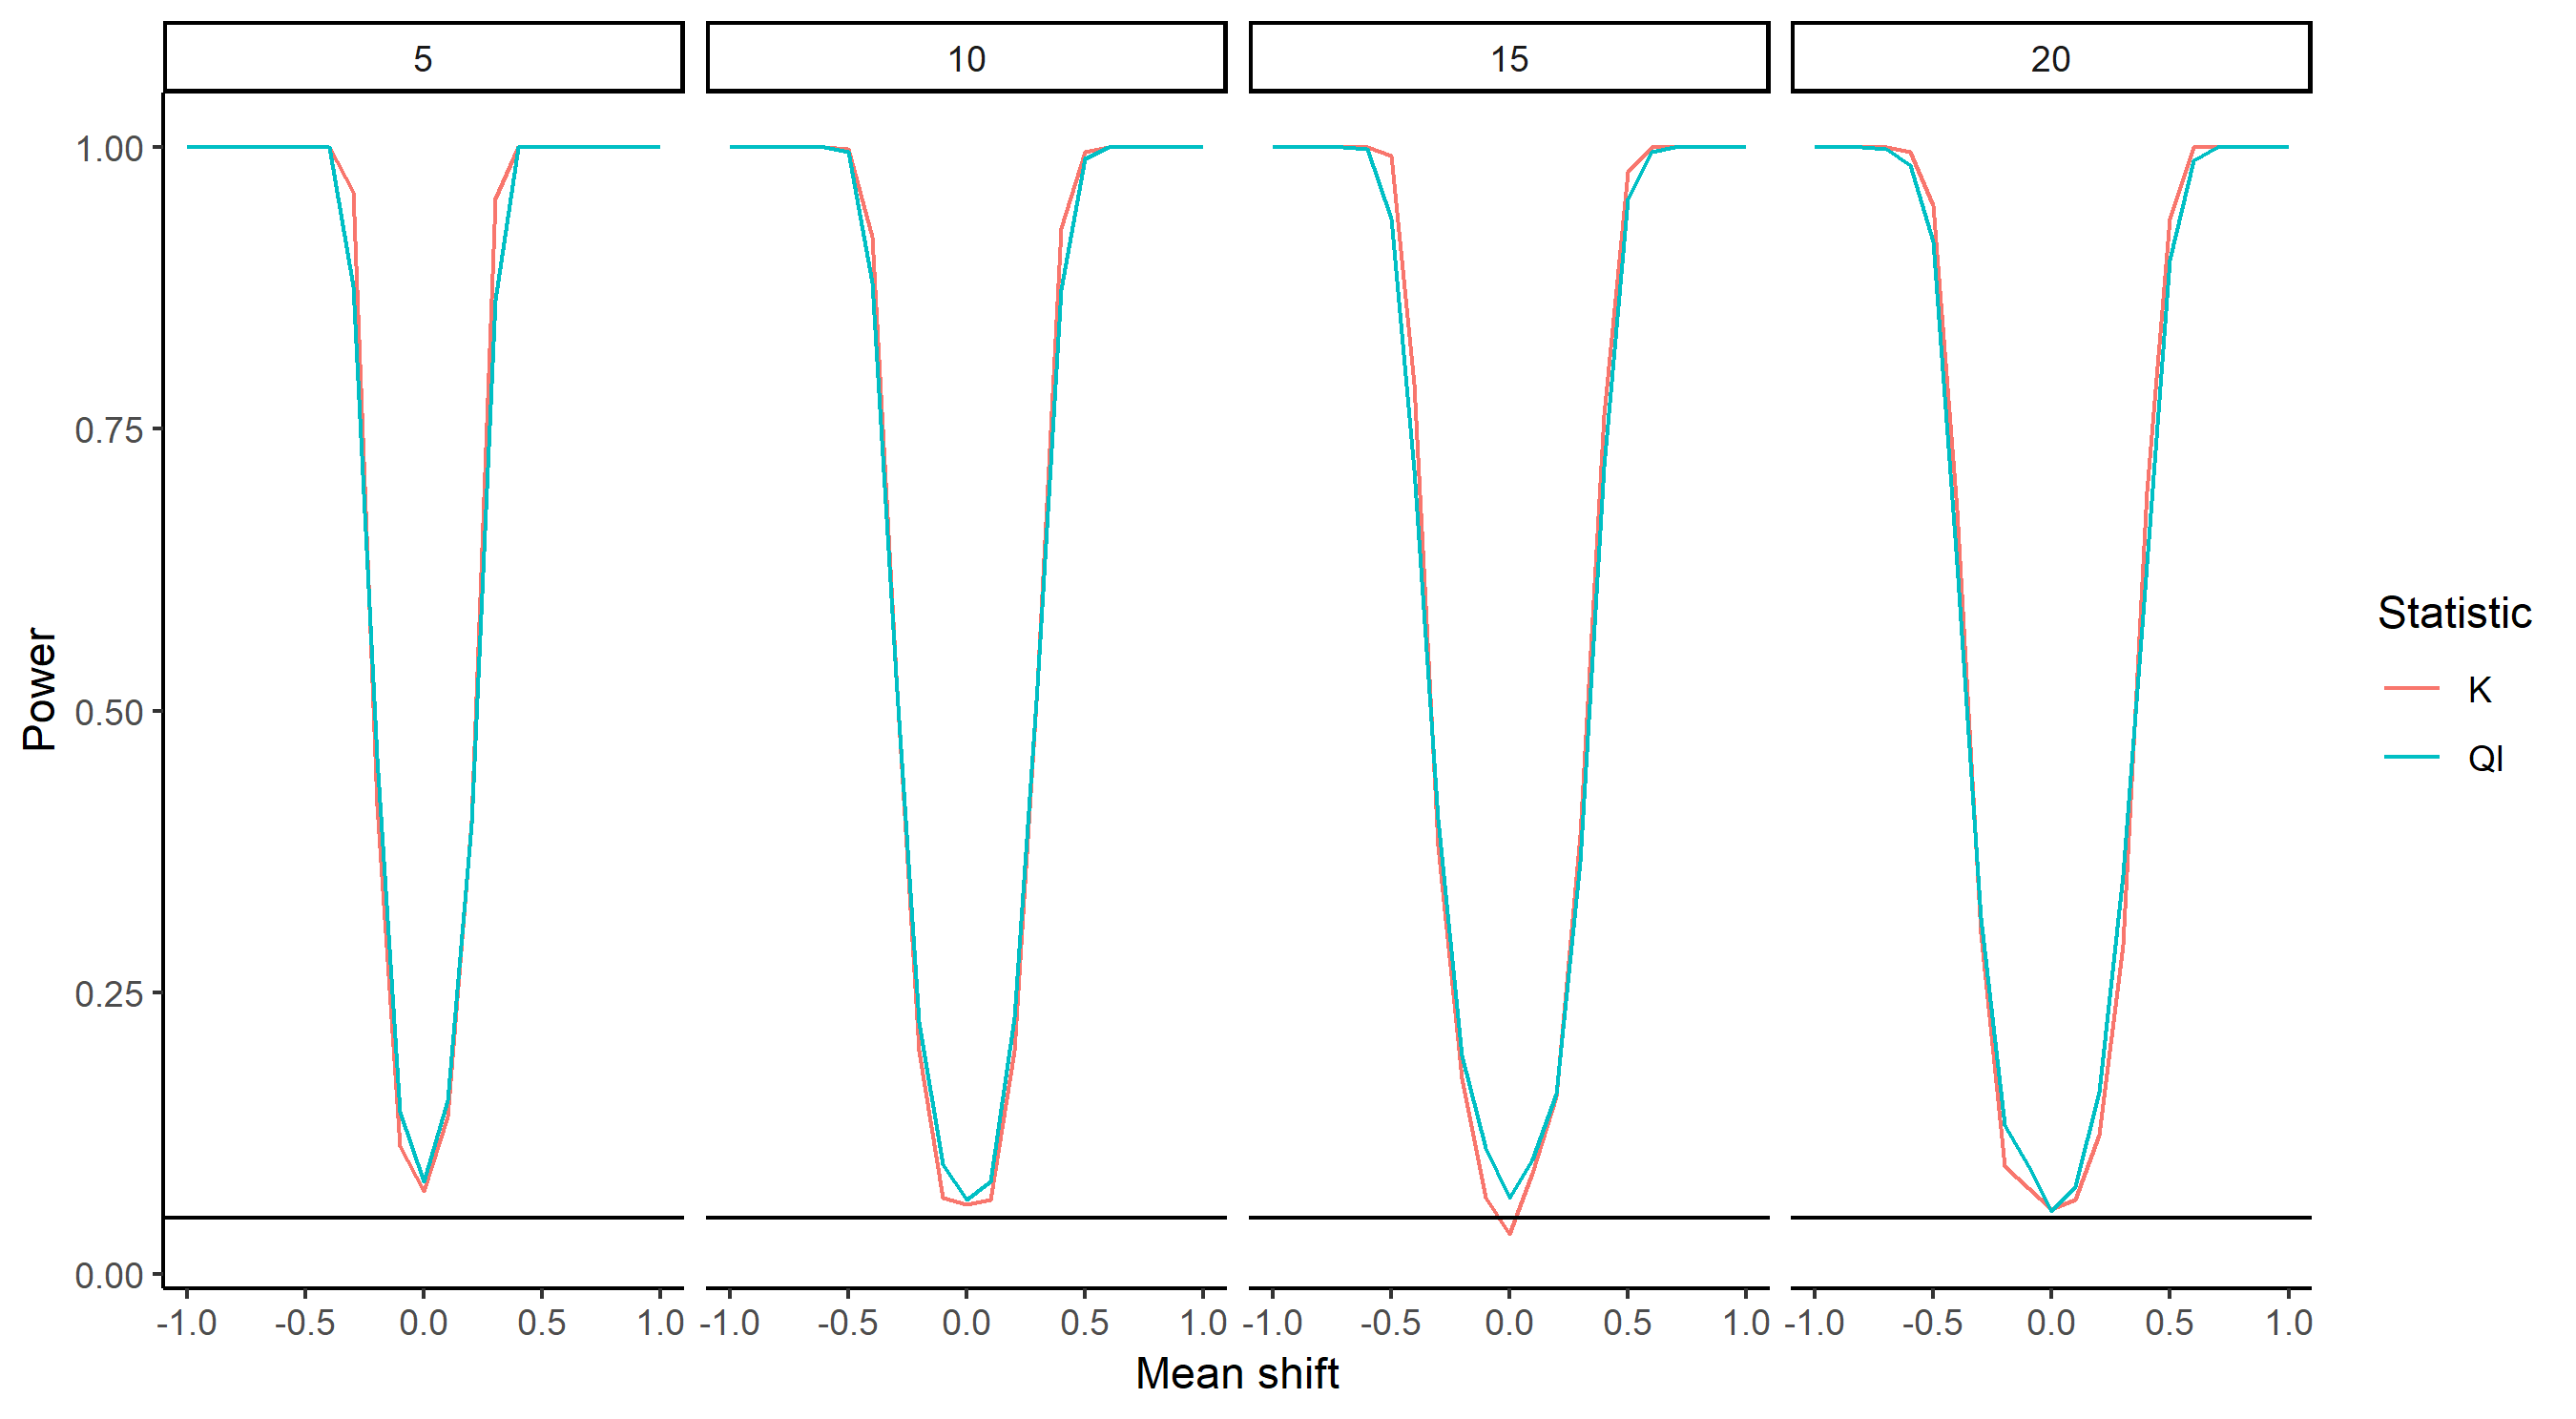
\includegraphics[width=0.6\textwidth,valign=c]{power/mu2d.png}
%     \caption{Power 2d mean}
%     \end{center}
% \end{figure}

% \begin{figure}[H]
% 	\begin{center}
%     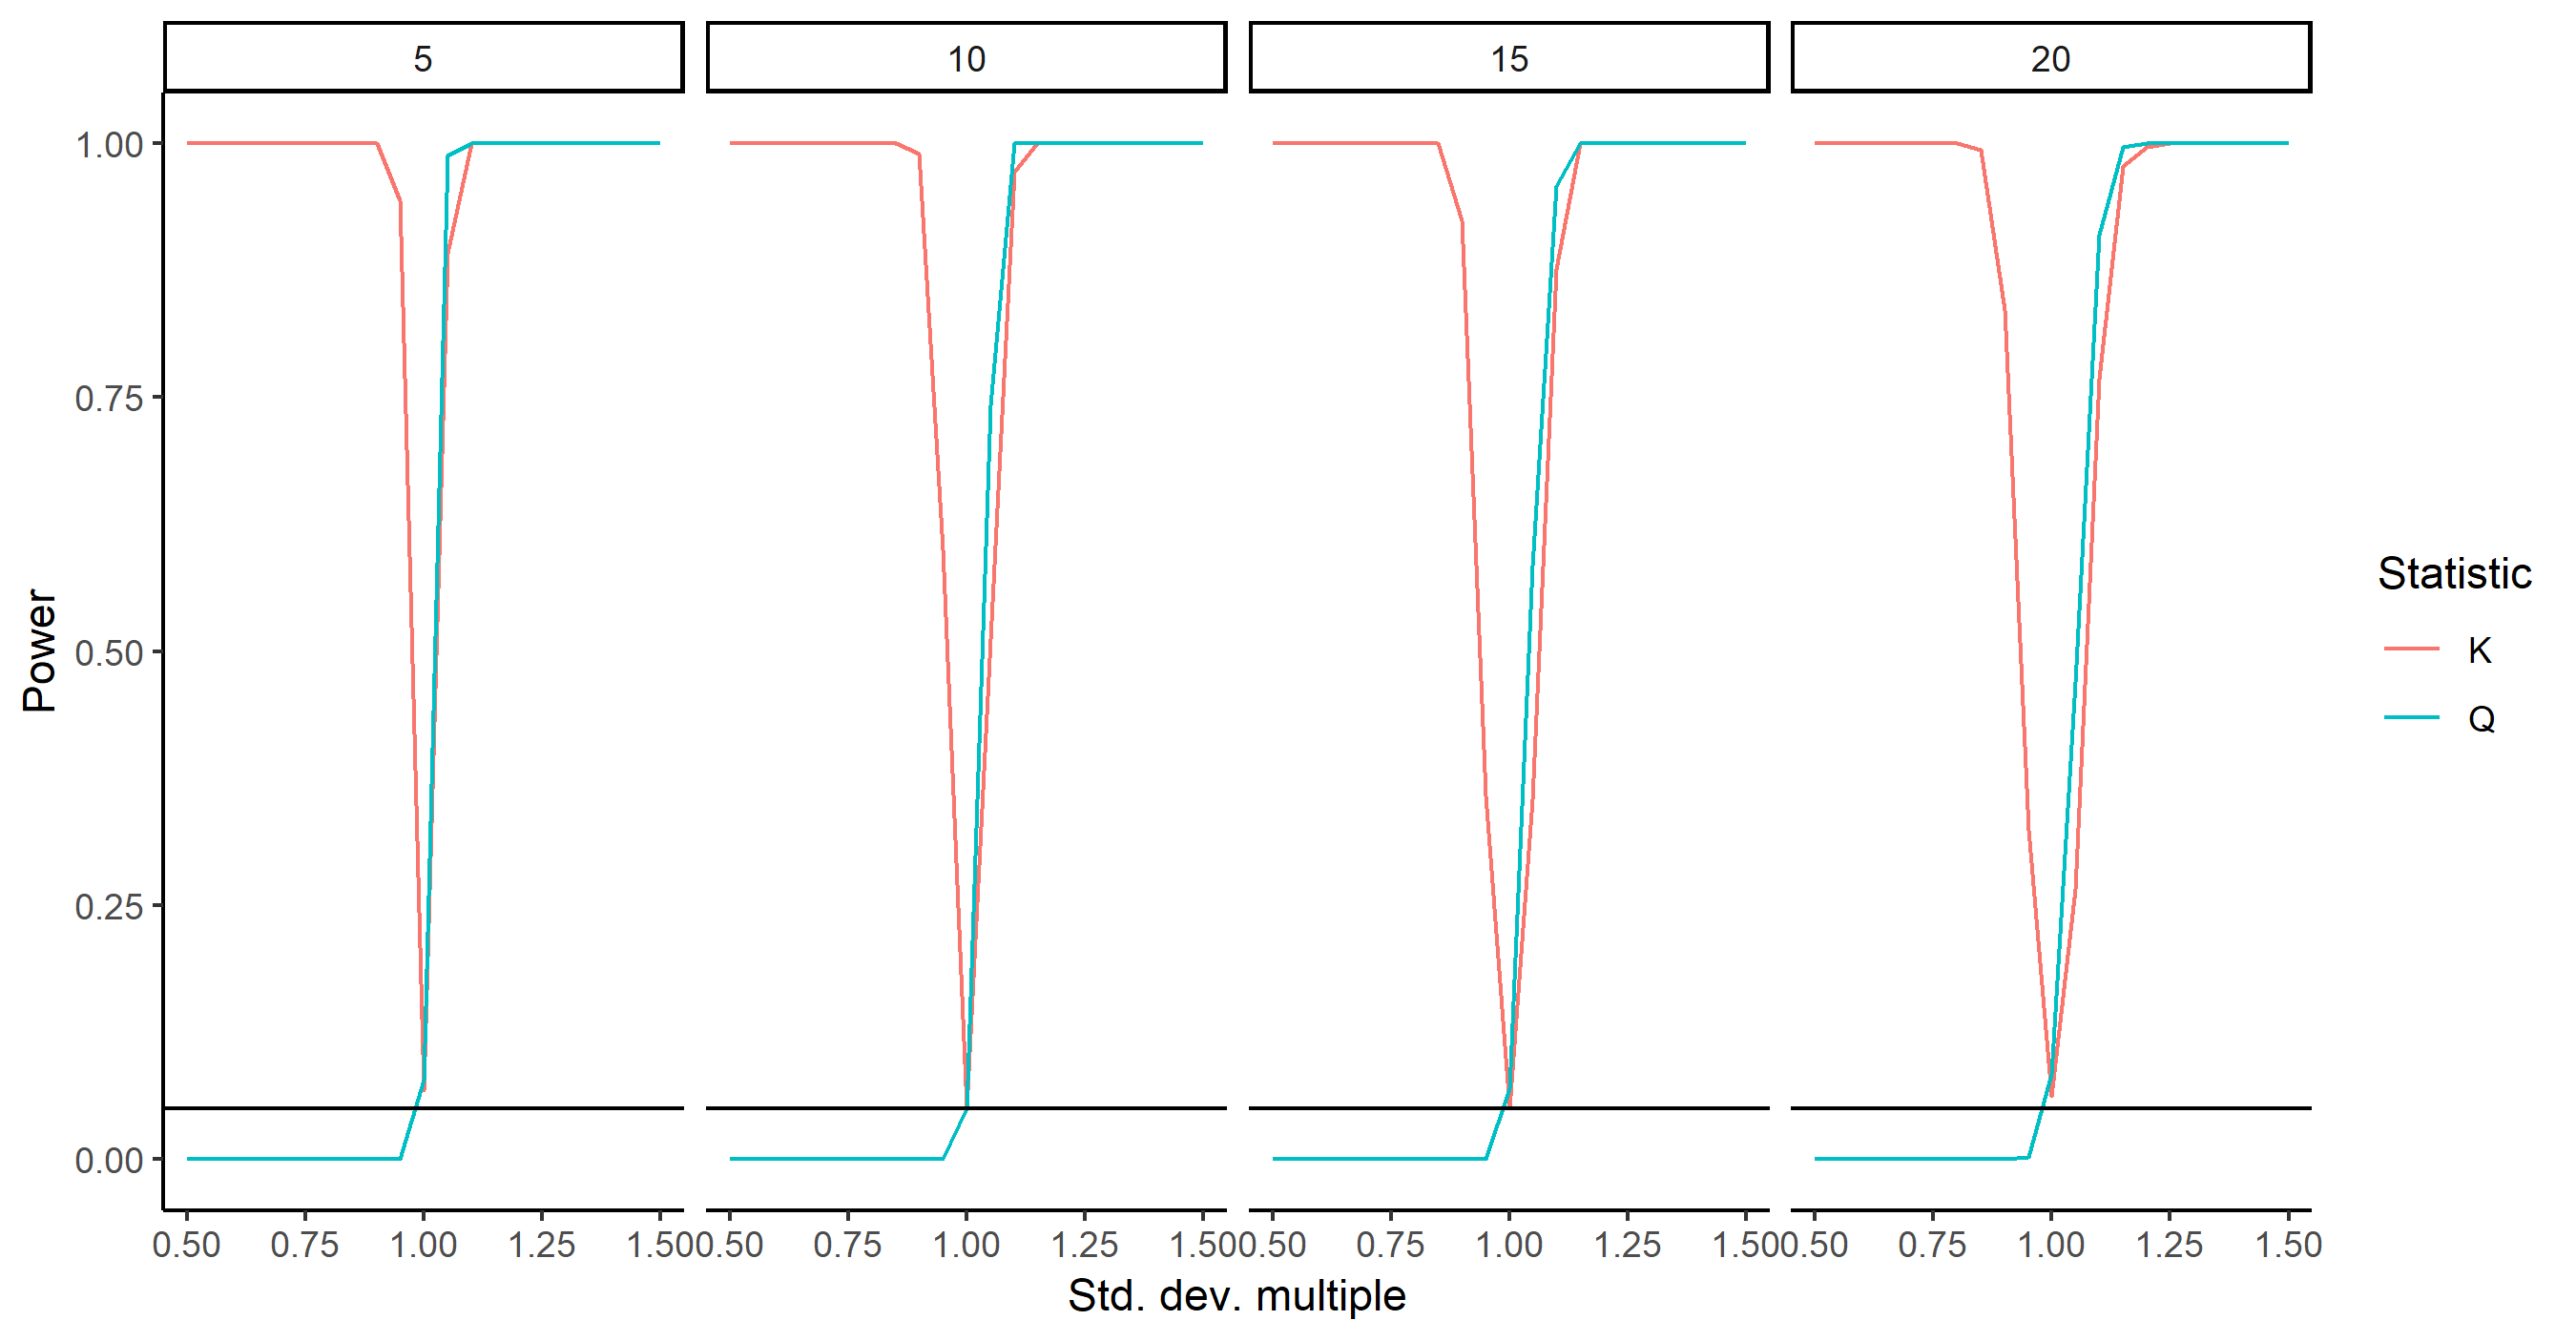
\includegraphics[width=0.6\textwidth,valign=c]{power/sd2d.png}
%     \caption{Power 2d sd}
%     \end{center}
% \end{figure}

% \begin{figure}[H]
% 	\begin{center}
%     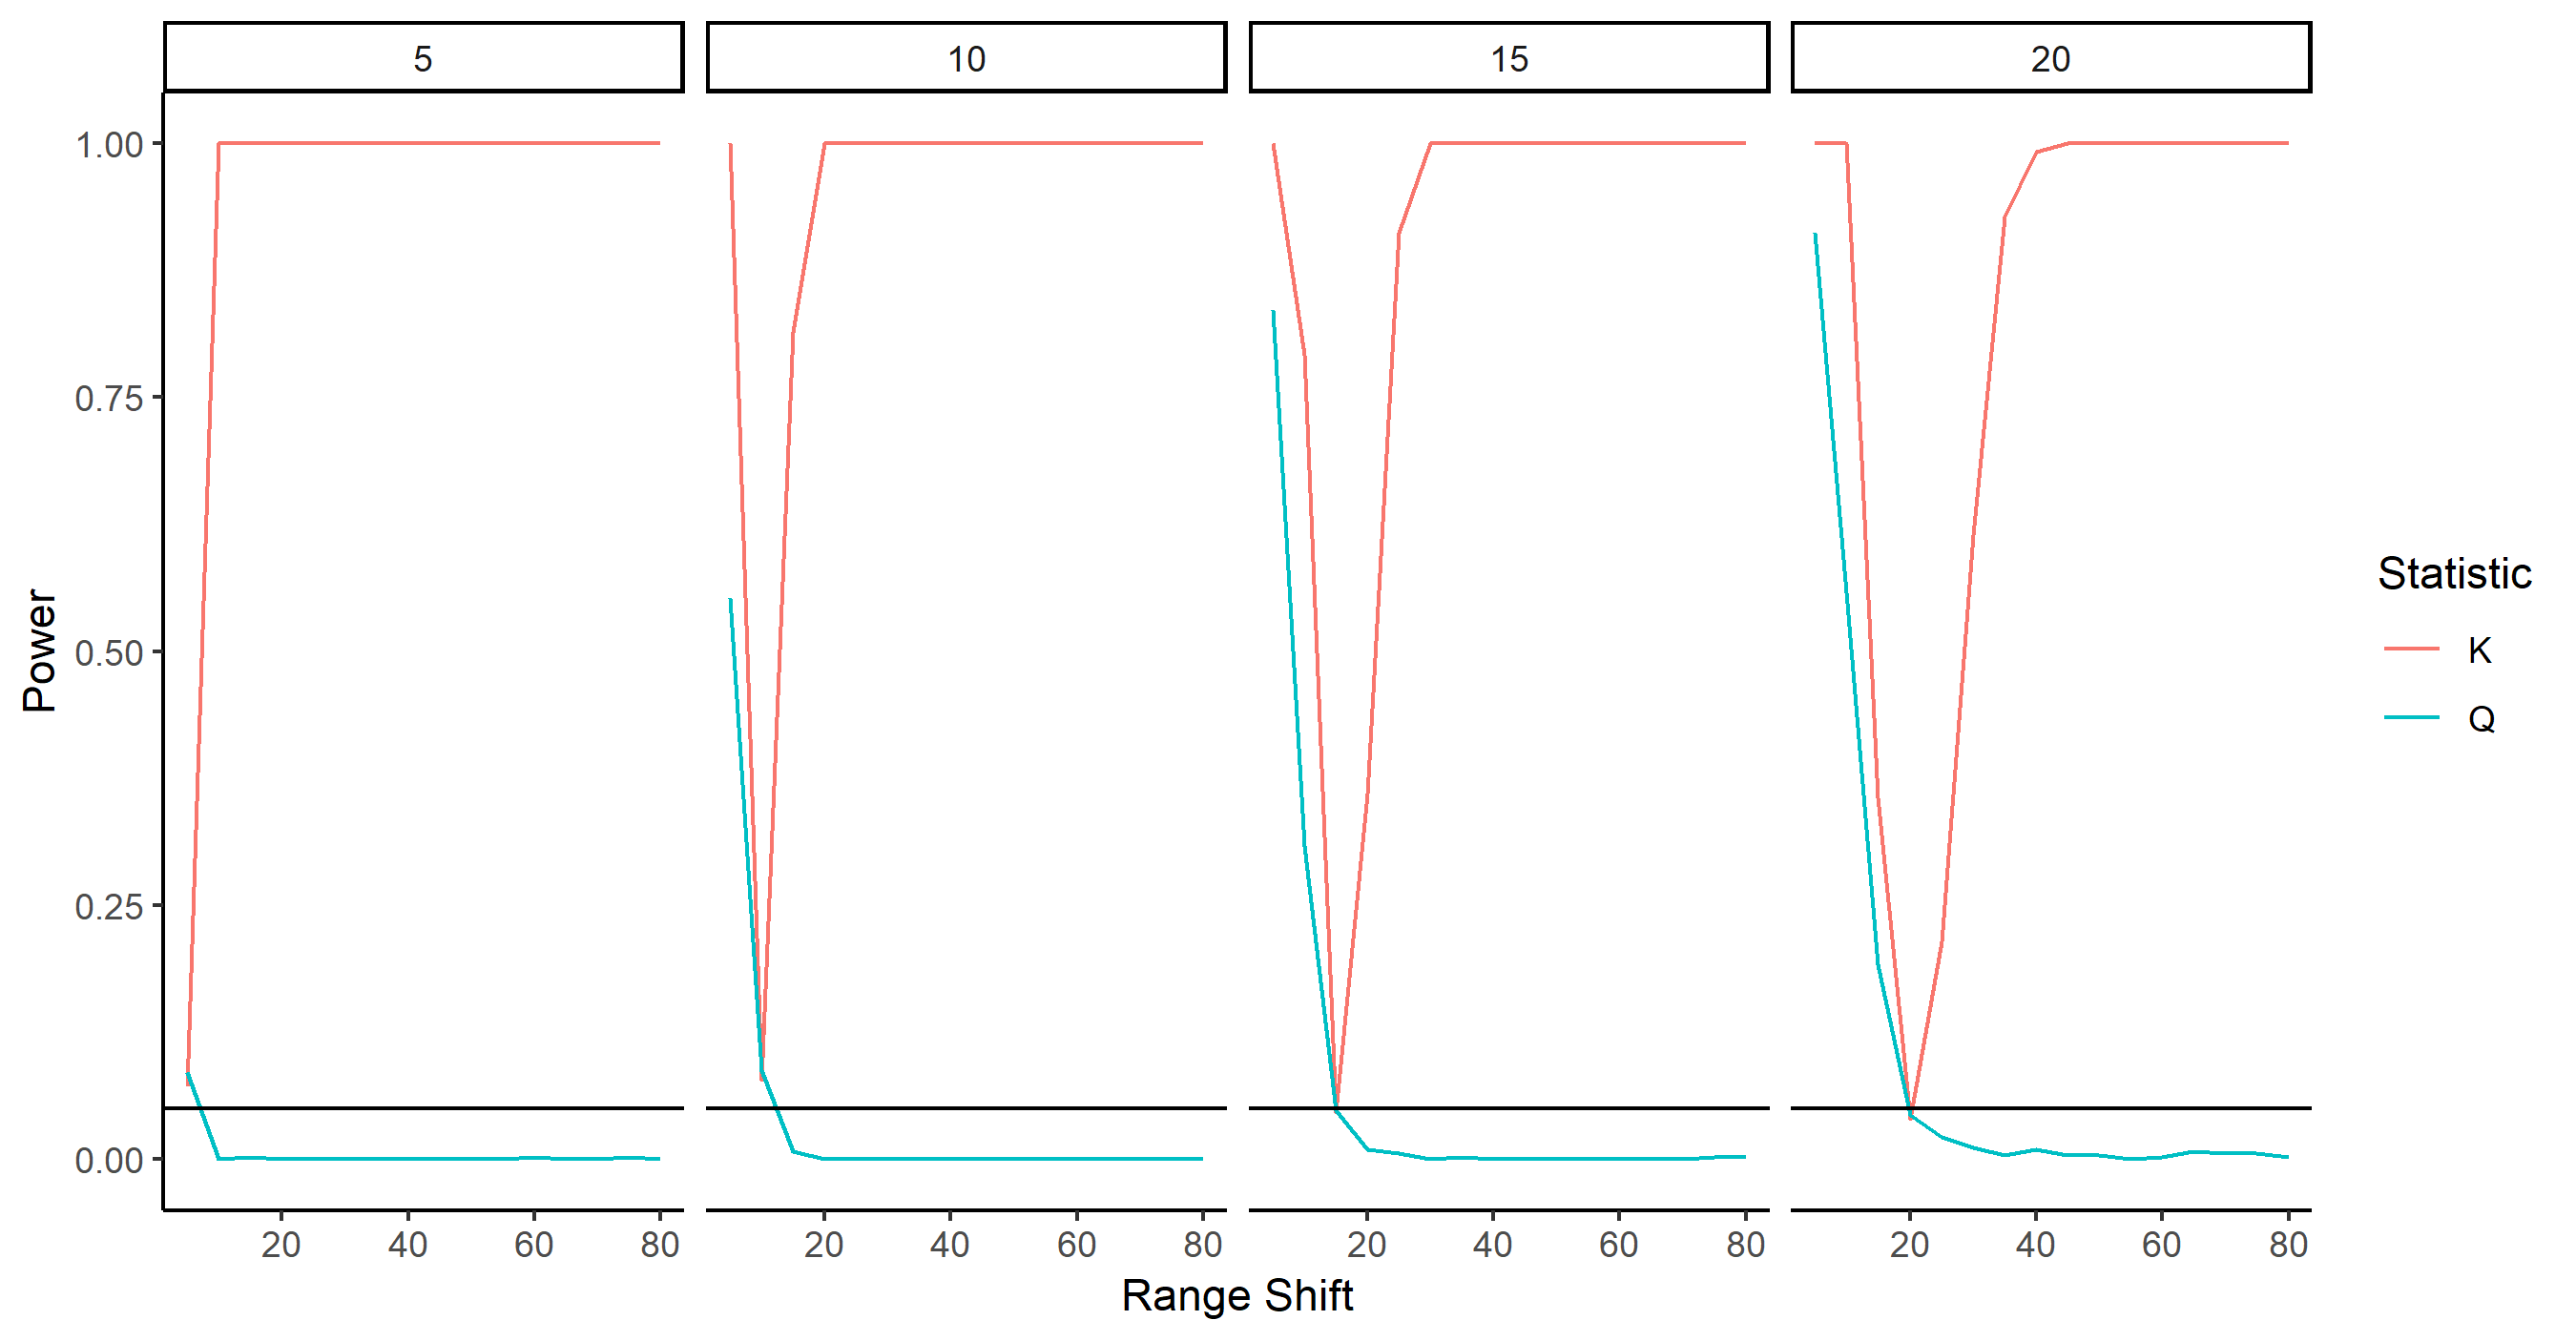
\includegraphics[width=0.6\textwidth,valign=c]{power/cr2d.png}
%     \caption{Power 2d range}
%     \end{center}
% \end{figure}

% \begin{figure}[H]
% 	\begin{center}
%     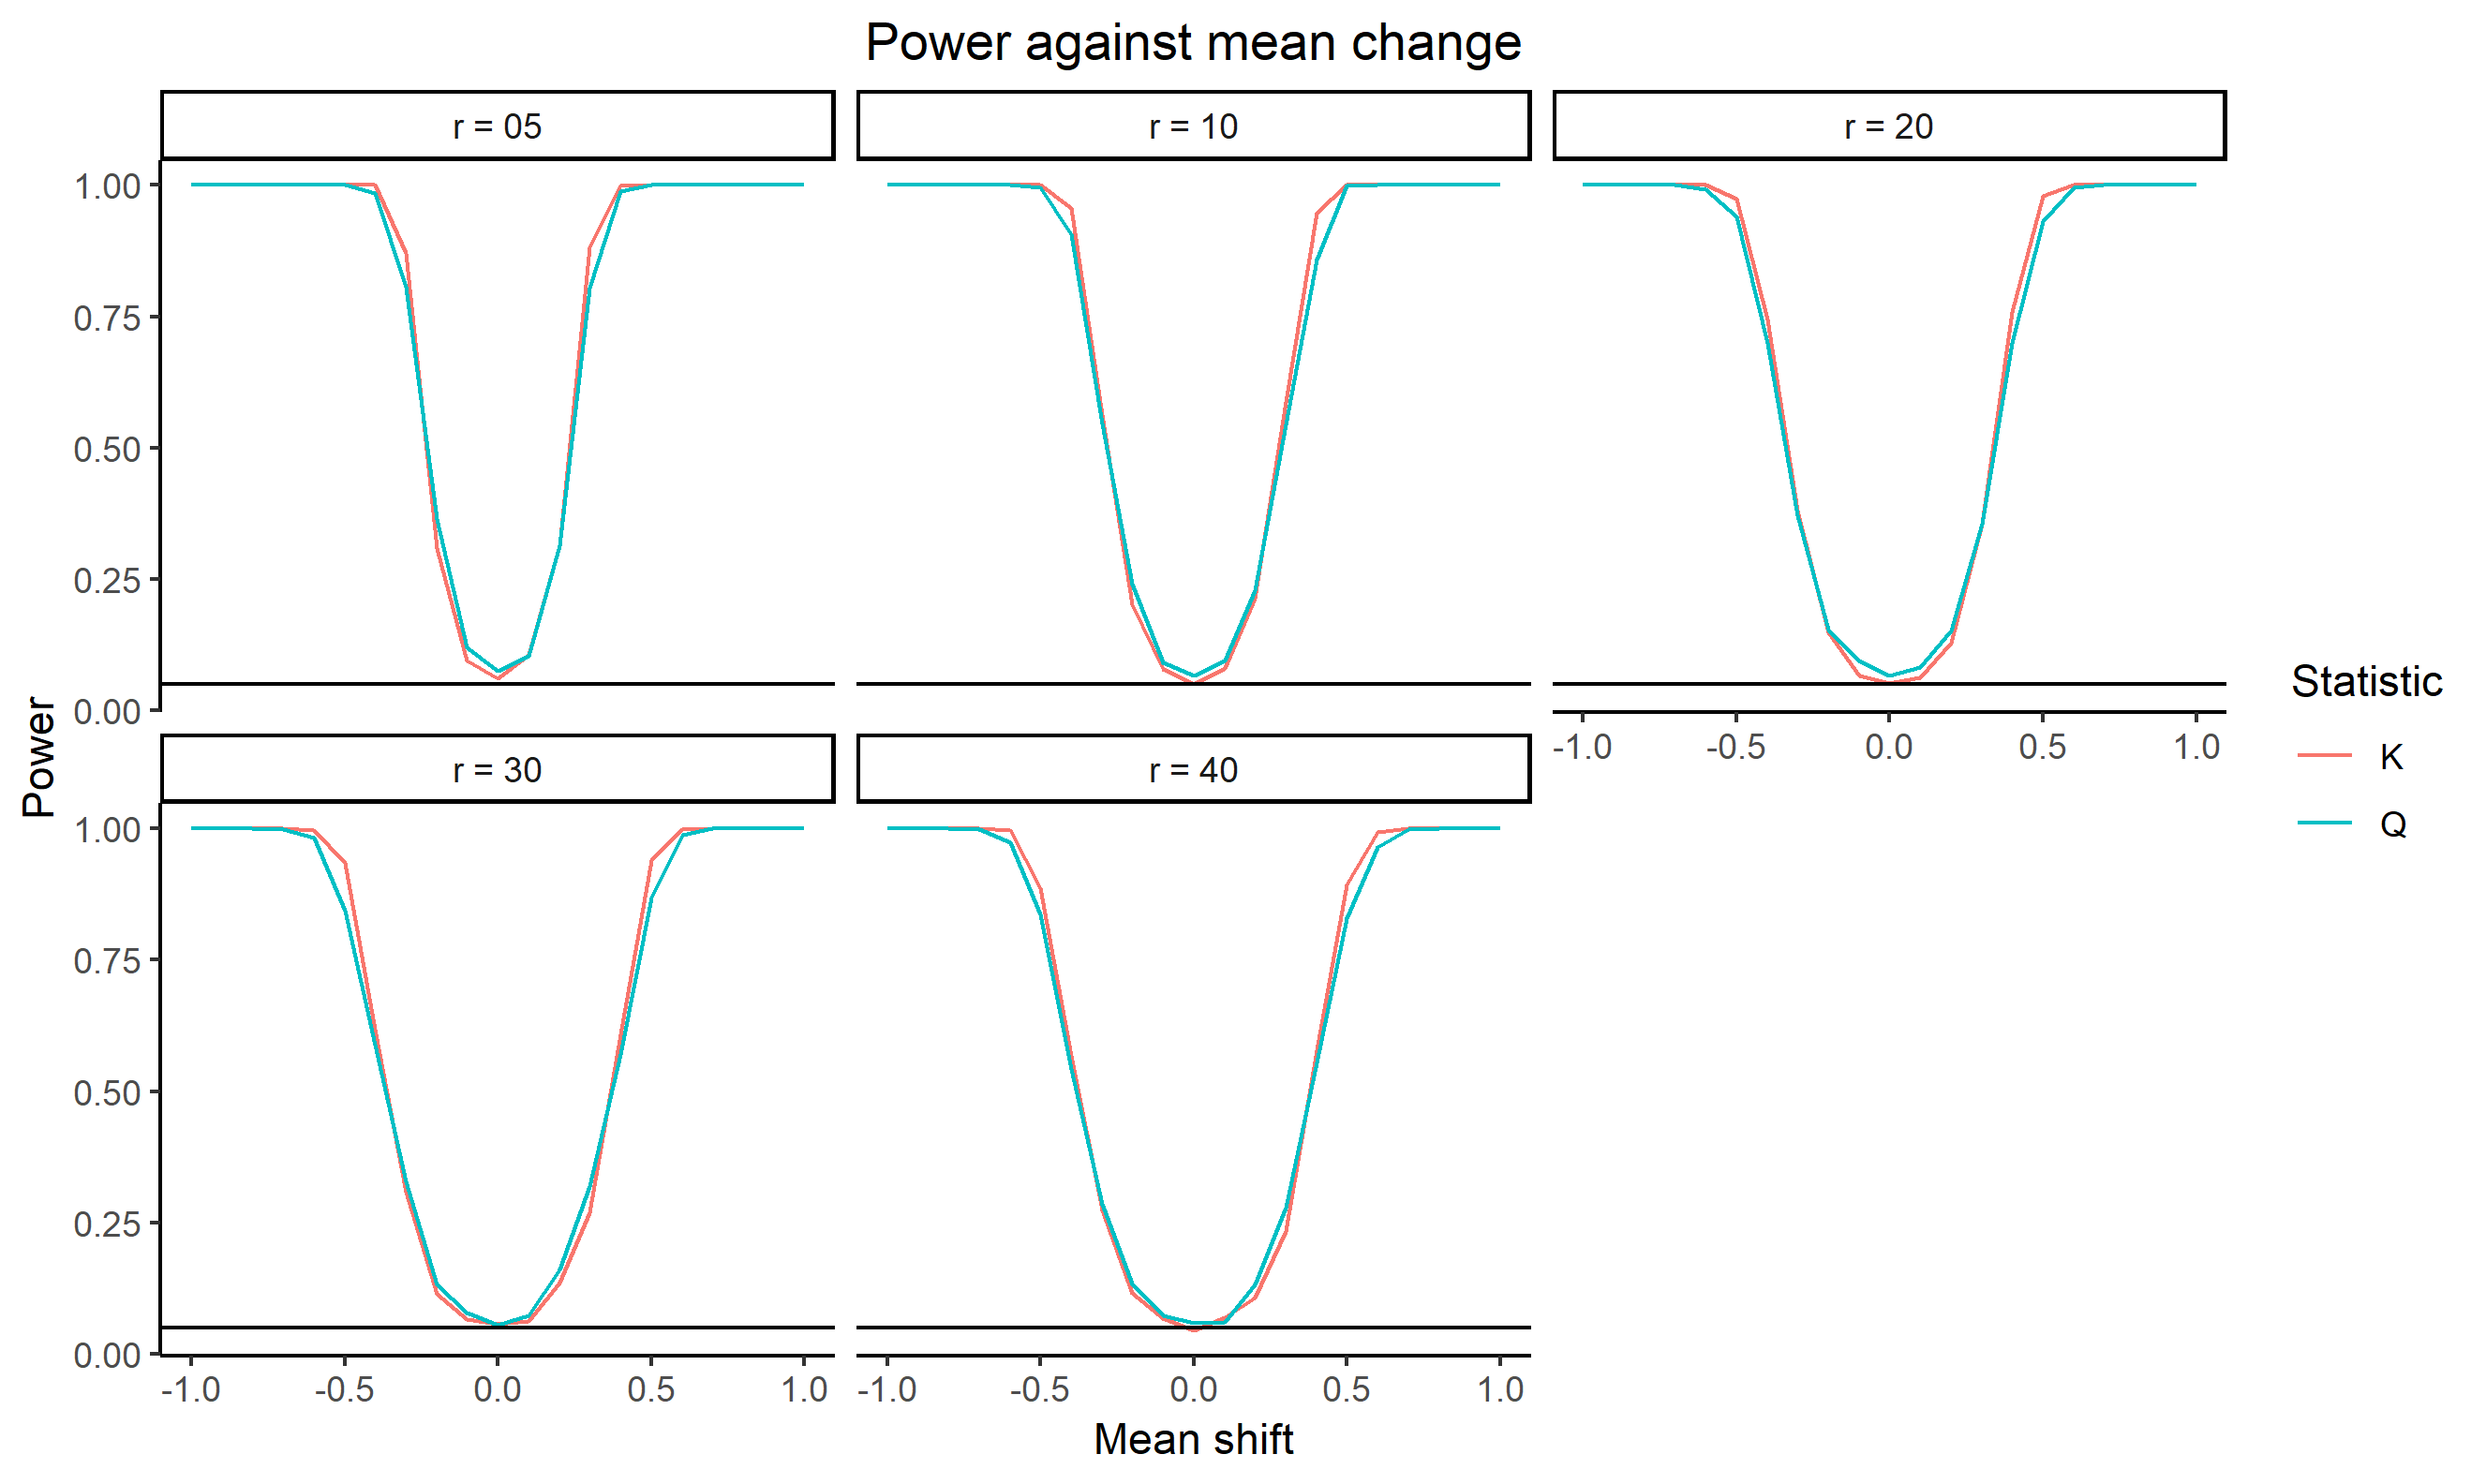
\includegraphics[width=0.6\textwidth,valign=c]{power/location1d_rng.png}
%     \caption{Power 1d mean}
%     \end{center}
% \end{figure}

% \begin{figure}[H]
% 	\begin{center}
%     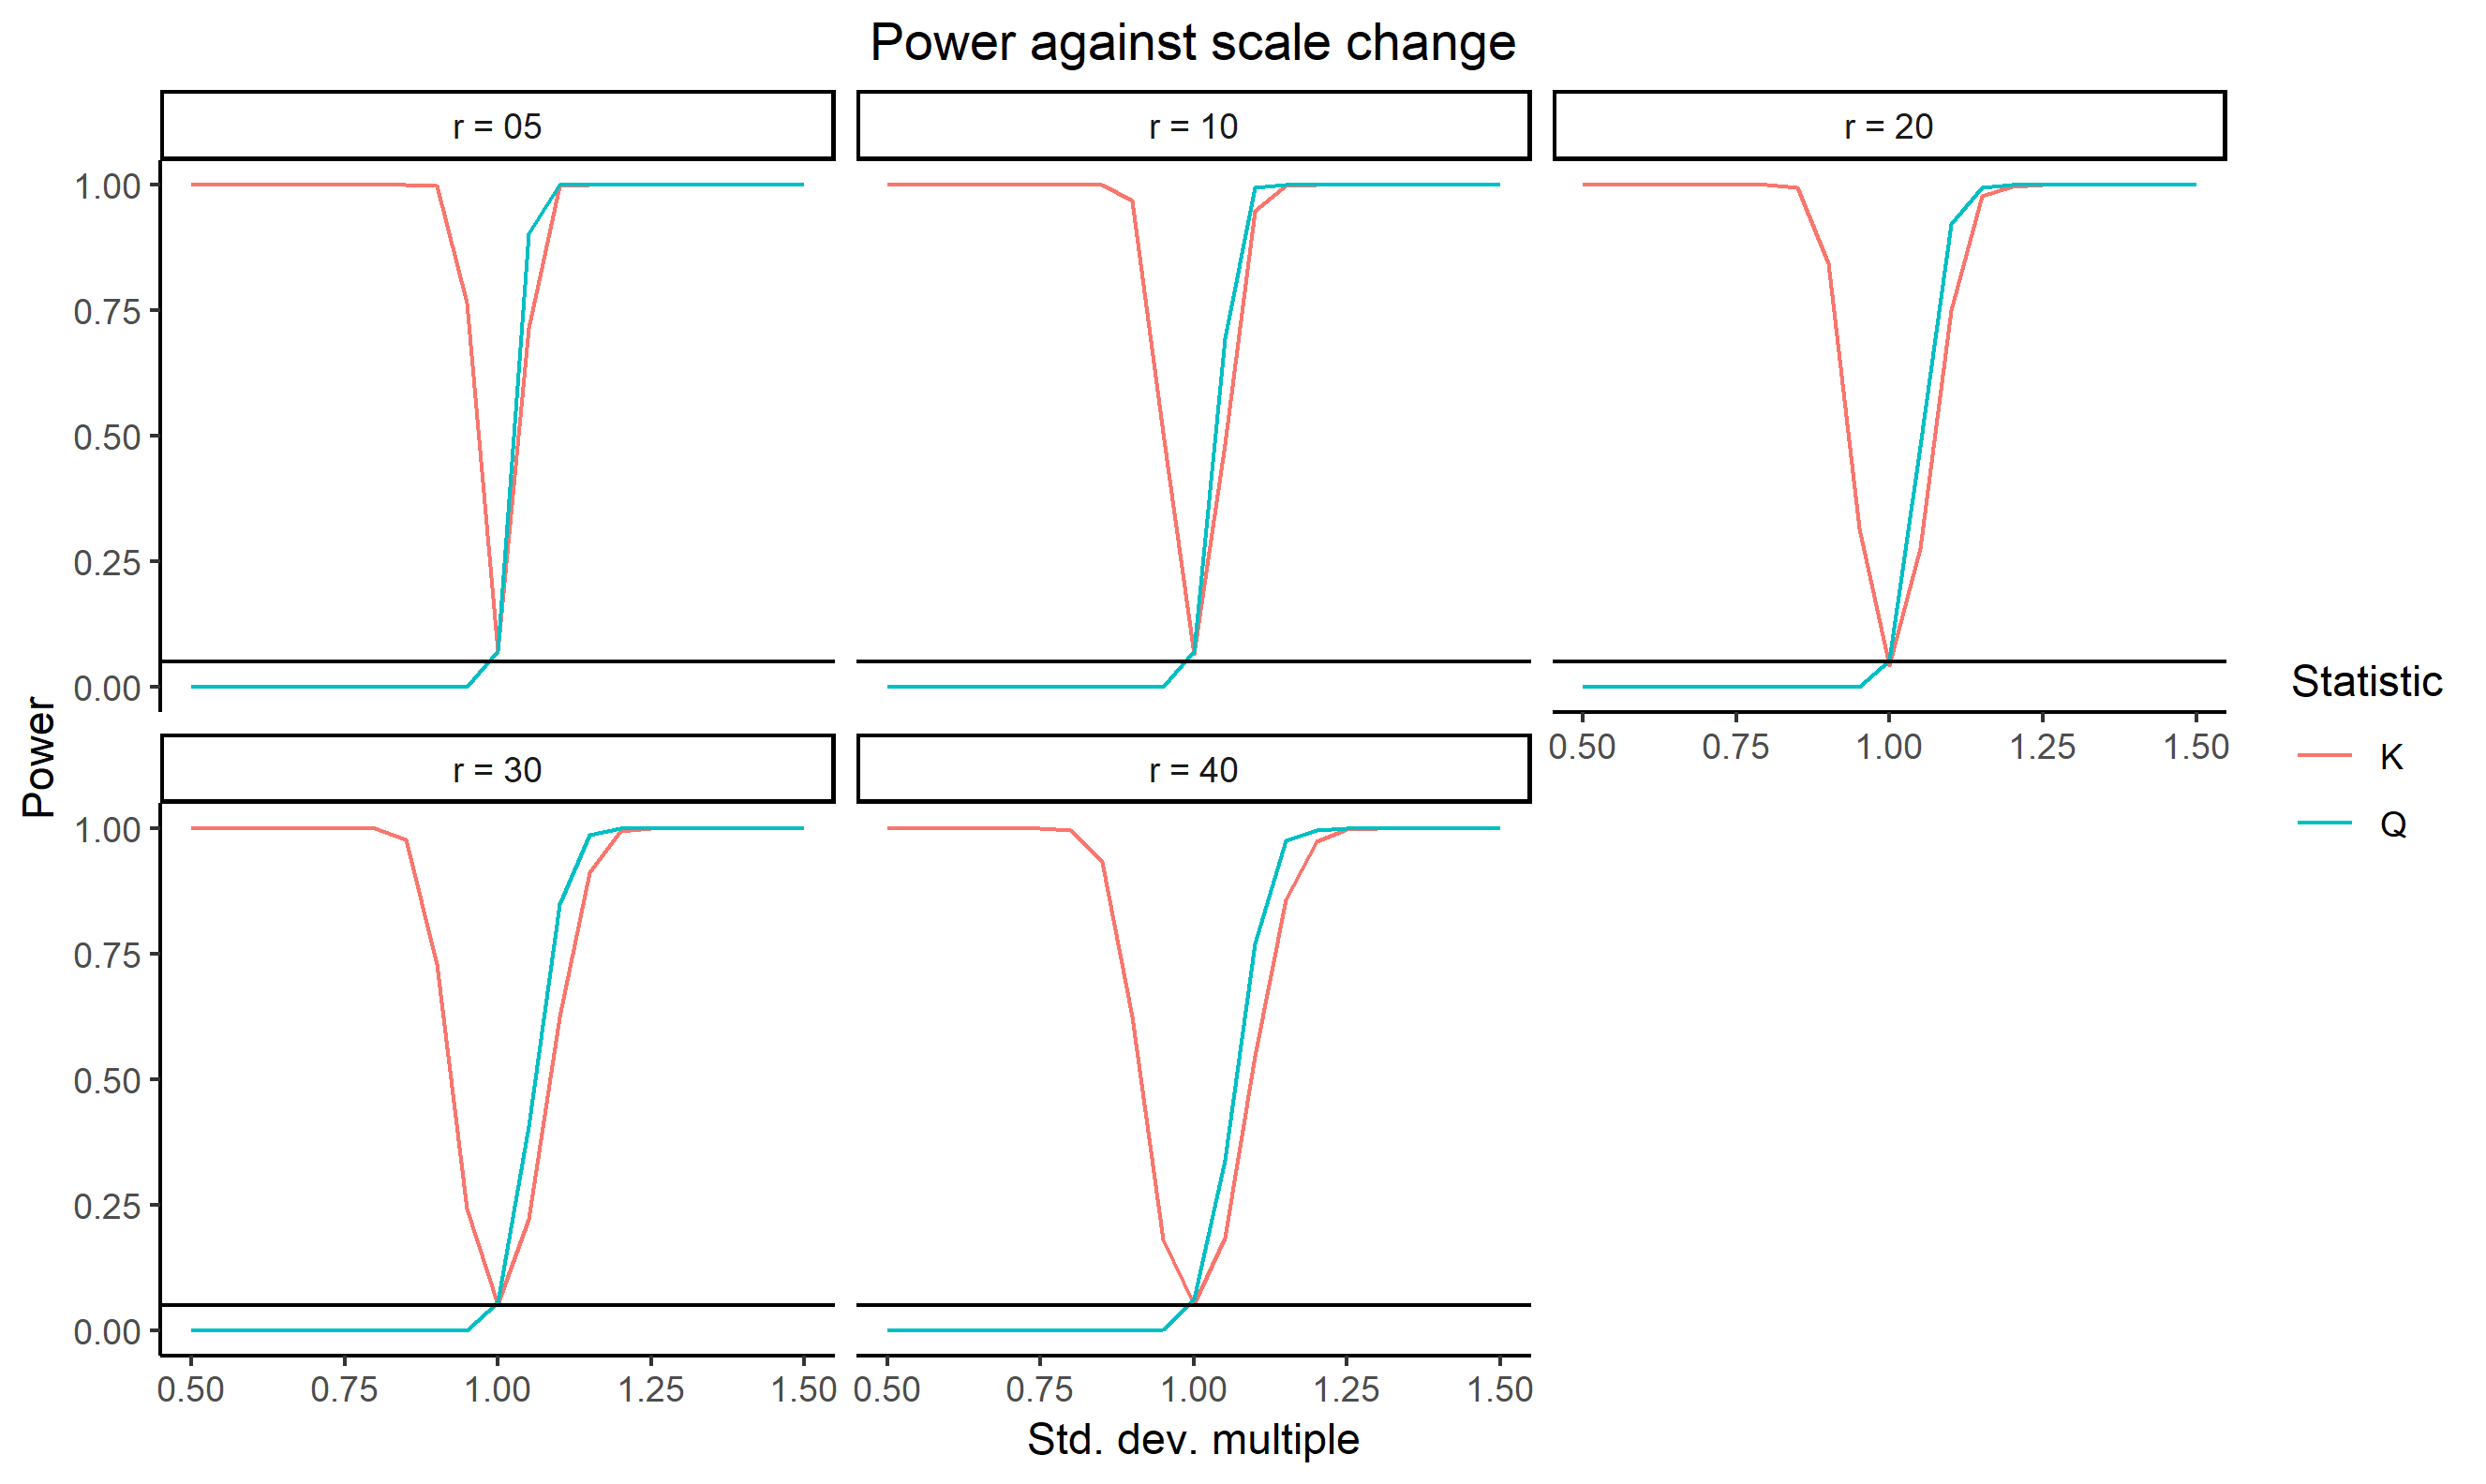
\includegraphics[width=0.6\textwidth,valign=c]{power/scale1d_rng.png}
%     \caption{Power 1d sd}
%     \end{center}
% \end{figure}

% \begin{figure}[H]
% 	\begin{center}
%     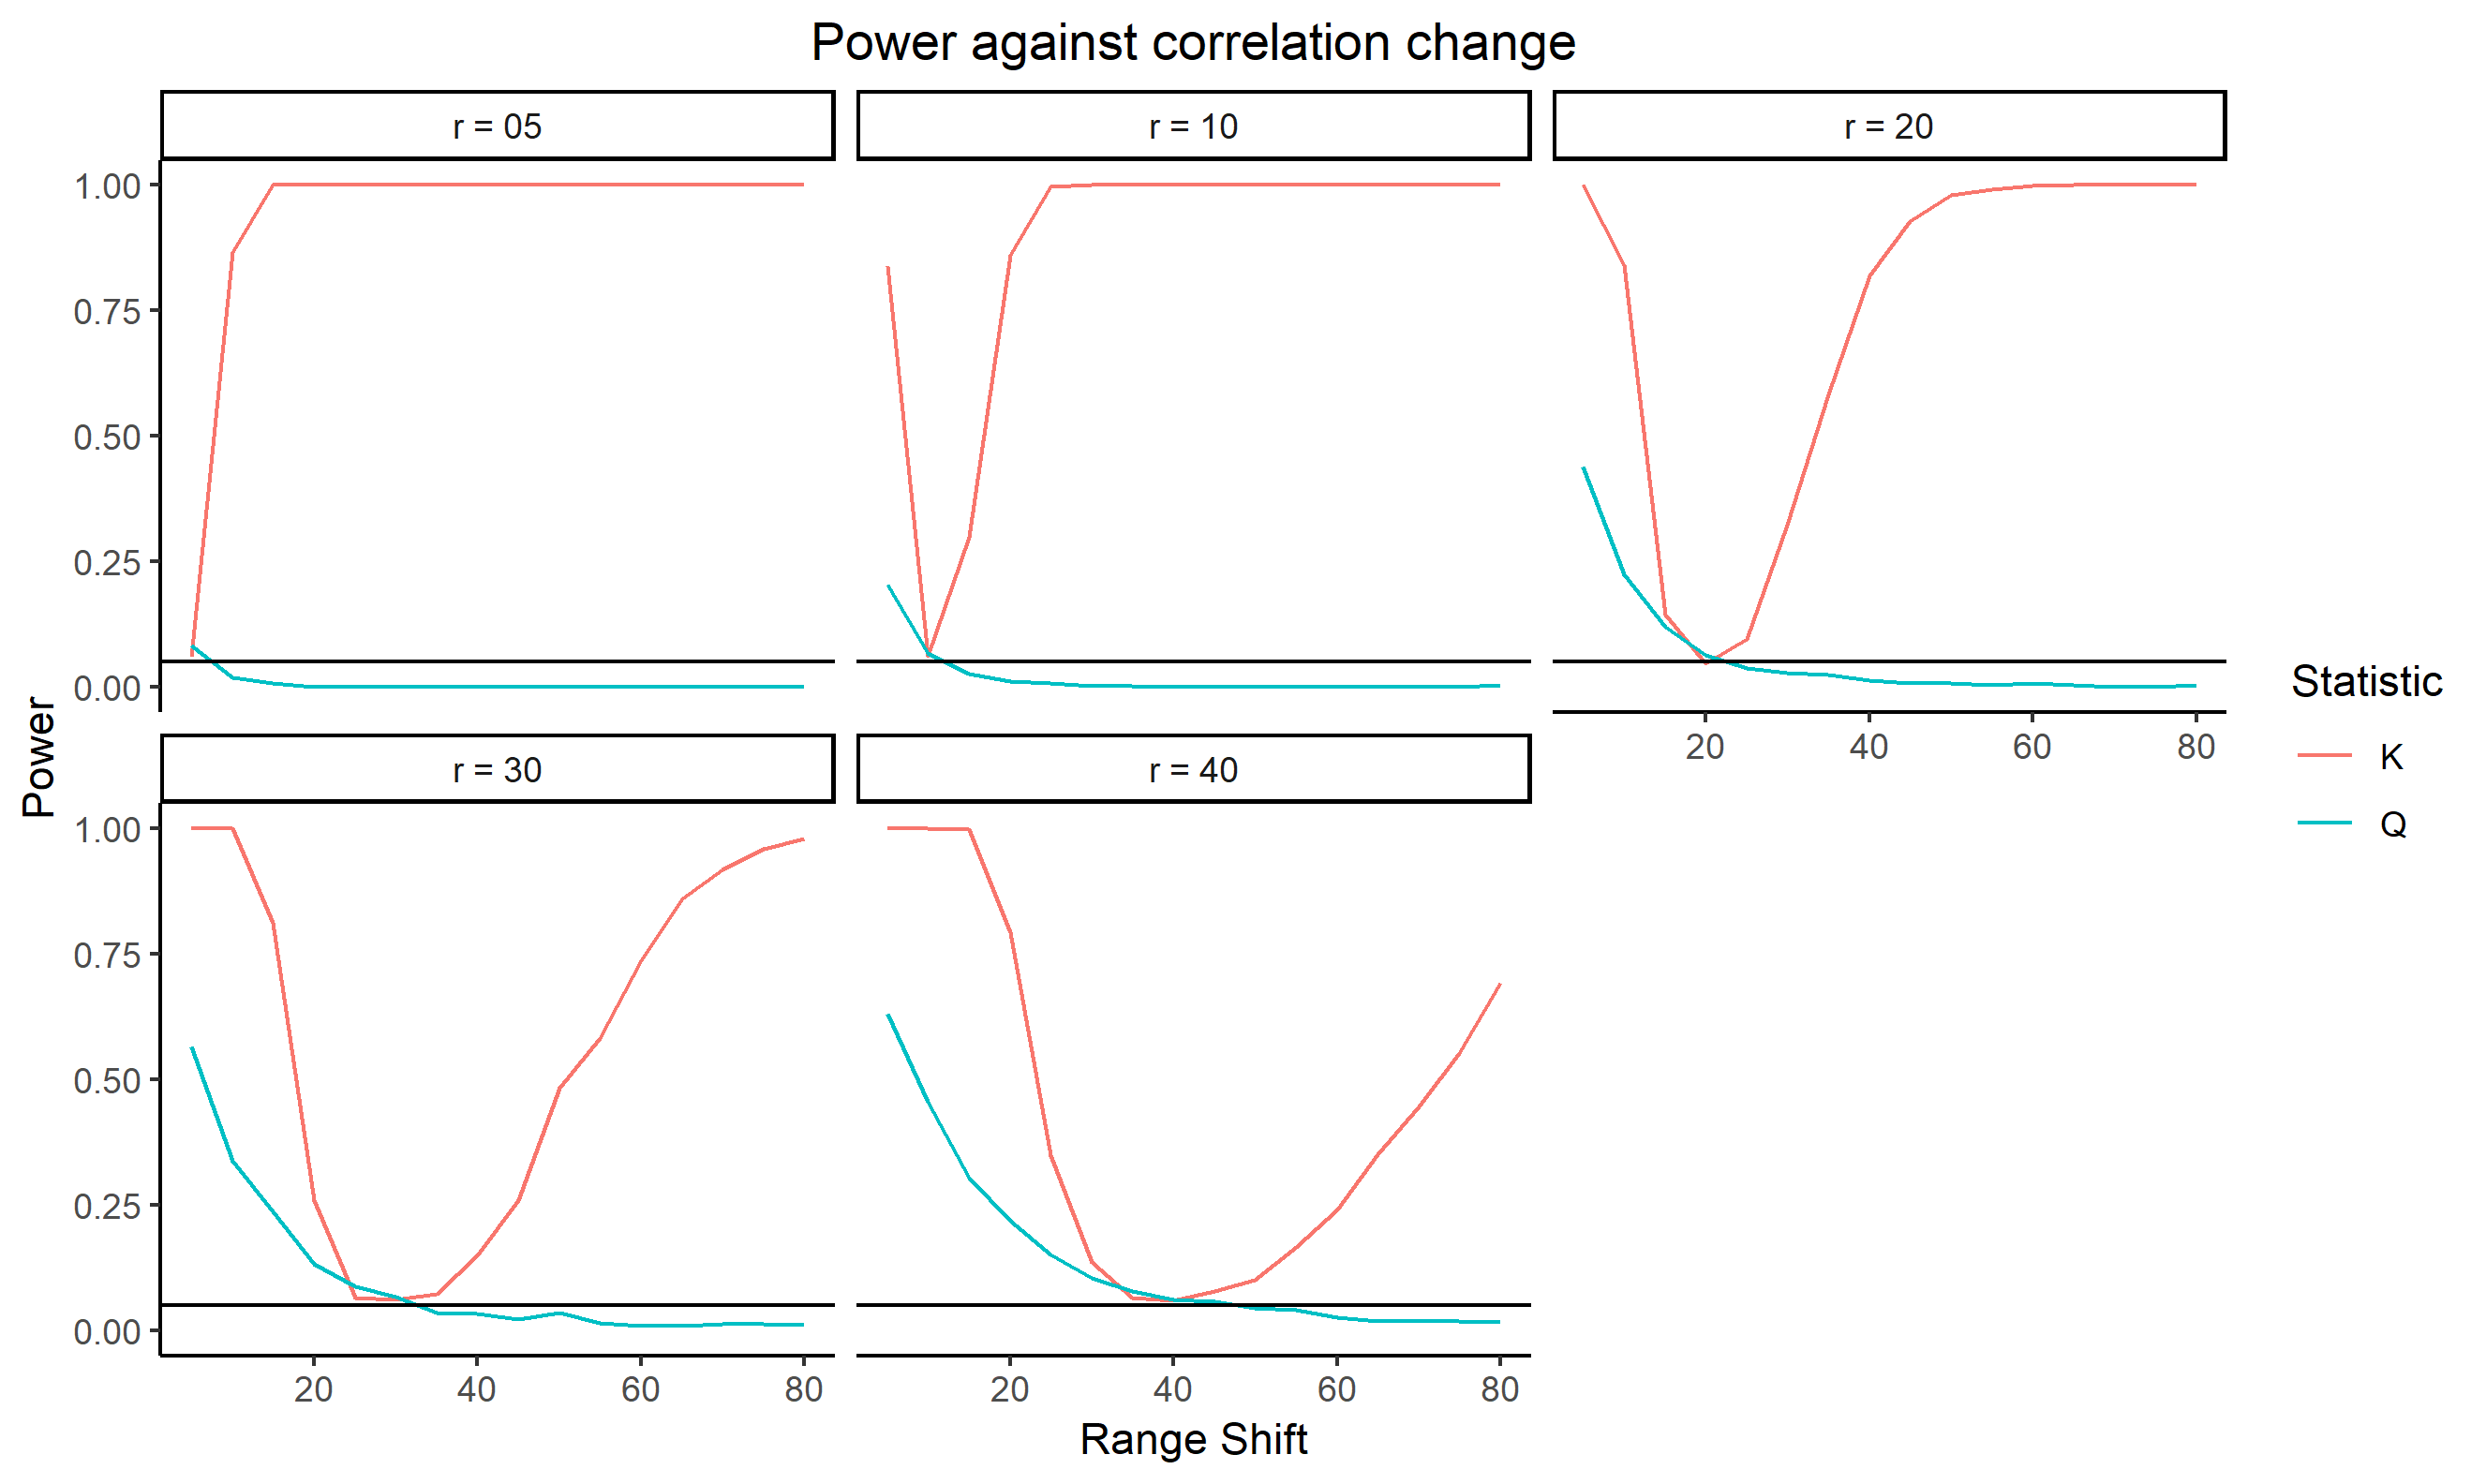
\includegraphics[width=0.6\textwidth,valign=c]{power/correlation1d_rng.png}
%     \caption{Power 1d range}
%     \end{center}
% \end{figure}

% \subsection{Proofs}
% To prove the following results we first reintroduce some notation. Let $P$ be some distribution on $C[0, 1]$ and let $X = \{X_1,...,X_n\}$ be an \textit{i.i.d} sample from $P$, having empirical distribution $P_n$. Similarly let $Q$ be another distribution on $C[0, 1]$ and let $Y = \{Y_1,...,Y_n\} \sim Q$, having empirical distribution $Q_n$. Let $\widehat{F}_n(t)$, $\widehat{G}_n(t)$, $\widetilde{F}_n(t)$, and $\widetilde{G}_n(t)$ be defined as in section 2.2 and let $\widehat{F}(t)$, $\widehat{G}(t)$, $\widetilde{F}(t)$, and $\widetilde{G}(t)$ be their respective counterparts using the population level depths, $D(\cdot, P)$ and  $D(\cdot, Q)$. For instance
% \begin{align*}
%     \widehat{F}_n(t) &= \frac{1}{n}\sum_{i=1}^n \mathbbm{1}(D(X_i, P_n) \leq t) \\
%     \widehat{F}(t) &= \frac{1}{n}\sum_{i=1}^n \mathbbm{1}(D(X_i, P) \leq t),
% \end{align*}
% etc. We have assumed here without loss of generality that $X$ and $Y$ have the same sample size. The depth function $D(\cdot, P)$ is always taken to be the integrated depth described in section 2.1. We also work under the null hypothesis that $P = Q$.
 
% \begin{lemma}
% If $t$ in $[0, 1]$ then $\sqrt{\frac{n}{2}} (\widehat{F}_n(t) - \widehat{F}(t)) \xrightarrow{P} 0$.
% \end{lemma}

% \begin{proof}
% To show convergence in $P$ we will instead show convergence in $L^1$.
%  \begin{align*}
%     E\left| \sqrt{\frac{n}{2}} (\widehat{F}_n(t) - \widehat{F}(t)) \right| &= E\left| \sqrt{\frac{n}{2}} \frac{1}{n}\sum_{i=1}^n \mathbbm{1}(D(X_i, P_n) \leq t) - \mathbbm{1}(D(X_i, P) \leq t) \right| \\
%     &\leq \frac{1}{\sqrt{2n}} \sum_{i=1}^n E\left| \mathbbm{1}(D(X_i, P_n) \leq t) - \mathbbm{1}(D(X_i, P) \leq t) \right|
% \end{align*}
% The inner absolute value term can be rewritten as the sum of two disjoint indicators due to the fact that it itself is an indicator on two disjoint events. Namely,
% \begin{align*}
%     \left| \mathbbm{1}(D(X_i, P_n) \leq t) - \mathbbm{1}(D(X_i, P) \leq t) \right| &= \mathbbm{1}(D(X_i, P_n) \leq t < D(X_i, P)) \\
%                               &\quad\quad + \mathbbm{1}(D(X_i, P) \leq t < D(X_i, P_n)).
% \end{align*}
% Therefore our inequality becomes 
% \begin{align*}
% E\left| \sqrt{\frac{n}{2}} (\widehat{F}_n(t) - \widehat{F}(t)) \right| &\leq  \frac{1}{\sqrt{2n}} \sum_{i=1}^n P(D(X_i, P_n) \leq t < D(X_i, P)) \\ 
%  &\quad\quad + \frac{1}{\sqrt{2n}} \sum_{i=1}^n P(D(X_i, P) \leq t < D(X_i, P_n)).
% \end{align*}
% We will concentrate on bounding the second series since the first is nearly identical. The U-statistic formulation of (citation) is useful here to decompose $D(X_i, P_n)$ into three parts 
% \[
% D(X_i, P_n) = \frac{1}{n} \sum_{k=1}^n h_i(X_k) + B_{1n} + B_{2n},
% \]
% where the $h(X_k)$ are $i.i.d$ and $B_{1n} + B_{2n} = o_p(\frac{1}{\sqrt{n}})$. Formally $h_i(X_k)$ is defined to be 
% \[
% h_i(X_k) = \int_{A_1} \mathbbm{1}(X_k(t) < X_i(t)) dt + \int_{A_2} \mathbbm{1}(X_k(t) > X_i(t)) dt 
% \]
% where $A_1 = \{t: F_t(X_i(t)) < \frac{1}{2}\}$, $A_2 = \{t: F_t(X_i(t)) > \frac{1}{2}\}$, and $F_t$ is the continuous univariate CDF defined on the projections $X(t)$ in section 2.2. $B_{1n}$ and $B_{2n}$ are defined similarly as 
% \begin{align*}
%     B_{1n} &=  \int_{A_1 \cap A_{2n}} [1 - 2\widehat{F}_{n,t}(X(t))]dt \\
%     B_{2n} &= \int_{A_2 \cap A_{1n}} [2\widehat{F}_{n,t}(X(t)) - 1]dt
% \end{align*}
% where $A_{1n} = \{t: \widehat{F}_{n,t}(X(t)) < \frac{1}{2}\}$, $A_{2n} = \{t: \widehat{F}_{n,t}(X(t)) > \frac{1}{2}\}$, and $\widehat{F}_{n,t}$ is the empirical estimator of $F_t$. We can use this decomposition to rearrange $P(D(X_i, P) \leq t < D(X_i, P_n))$ as
% \begin{align*}
%   P(D(X_i, P) \leq t < D(X_i, P_n)) &= P(D(X_i, P_n) -  D(X_i, P) > t - D(X_i, P) \geq 0) \\
%   &= P \left( \frac{1}{n} \sum_{k=1}^n \left[ h_i(X_k) + B_{1n} + B_{2n} - D(X_i, P) \right] > t - D(X_i, P) \geq 0 \right) \\
%   &= P \left( \frac{1}{n} \sum_{k=1}^n \left[ h_i(X_k) - D(X_i, P) \right] > t - D(X_i, P) \geq 0 \right). \\
%   &= E \left[ P \left( \frac{1}{n} \sum_{k=1}^n \left[ h_i(X_k) - D(x, P) \right] > t - D(x, P) \geq 0 \middle| X_i = x \right) \right].
% \end{align*}
% Since $h_i(X_i) = 0$,  this can be written as the sum of $n - 1$ i.i.d variables
% \[
% E_X \left[ P \left( \frac{1}{n-1} \sum_{k \neq i} \left[ h_i(X_k) - D(x, P) \right] > \frac{n}{n-1}(t - D(x, P)) \geq 0 \middle| X_i = x \right) \right]. \\
% \]
% Note that $E[D(X_i, P_n) - D(X_i, P)] = 0$ and $D(X_i, P_n) - D(X_i, P)$ is bounded between $[-1, 1]$. Since $t - D(X_i, P) \geq 0$ we can apply Hoeffding's inequality to the inner probability to get the upper bound 
% \[
% P \left( \frac{1}{n-1} \sum_{k \neq i} \left[ h_i(X_k) - D(x, P) \right] > \frac{n}{n-1}(t - D(x, P)) \geq 0 \middle| X_i = x \right) \leq \text{exp}\left( -\frac{n}{2}(t - D(x, P))^2 \right).
% \]
% Furthermore, since $D(X_i, P)$ is bounded between $[0, 1]$ it's sub Gaussian so there exists some constant $C < \infty$ such that 
% \[
% E_X \left[\text{exp}\left( -\frac{n}{2}(t - D(x, P))^2 \right) \right] \leq \text{exp}\left( -\frac{n}{2}C \right)
% \]
% A similar result holds for $P(D(X_i, P_n) \leq t < D(X_i, P))$, so our inequality becomes
% \begin{align*}
%         E\left| \sqrt{\frac{n}{2}} (\widehat{F}_n(t) - \widehat{F}(t)) \right| &\leq \frac{1}{\sqrt{2n}} \sum_{i=1}^n 2 e^{-\frac{n}{2}C} \\
%         &= \sqrt{2n} e^{-\frac{n}{2}C}. \\
%         &\rightarrow 0, \quad n \rightarrow \infty.
% \end{align*}
% Thus $\sqrt{\frac{n}{2}} (\widehat{F}_n(t) - \widehat{F}(t)) \xrightarrow{P} 0$ by Markov's inequality.
% \end{proof}

% \begin{lemma}
% If $t$ in $[0, 1]$ then $\sqrt{\frac{n}{2}} (\widehat{F}_n(t) - \widehat{G}_n(t)) \xrightarrow{D} N(0, F(t)(1-F(t))$ where $F(t) = P(D(X, P) < t)$.
% \end{lemma}

% \begin{proof}
% We start by showing that $\sqrt{n}(\widehat{F}(t) - F(t)) \xrightarrow{D} N(0, F(t)(1-F(t))$. Note that $\widehat{F}(t)$ is the mean of \textit{i.i.d} random variables $\mathbbm{1}(D(x_i, P) \leq t))$, since the $X_i$ are \textit{i.i.d} and $D(\cdot, P)$ does not depend on the rest of the sample. By definition
% \begin{align*}
%   E[\mathbbm{1}(D(x_i, P) \leq t))] &= F(t) \\
%   Var[\mathbbm{1}(D(x_i, P) \leq t))] &= F(t) - F(t)^2,
% \end{align*}
% so by the central limit theorem $\sqrt{n}(\widehat{F}(t) - F(t)) \xrightarrow{D} N(0, F(t)(1-F(t))$.
% With a nearly identical argument it can also be shown that $\sqrt{n}(\widehat{G}(t) - G(t)) \xrightarrow{D} N(0, G(t)(1-G(t))$. Under the null $X$ and $Y$ have the same distribution which implies that their depths do too, since depth is a deterministic function of $X$ and $Y$. Therefore $\sqrt{n}(\widehat{G}(t) - F(t)) \xrightarrow{D} N(0, F(t)(1-F(t))$. Moreover, since $X$ and $Y$ are independent 
% \[
% \sqrt{\frac{n}{2}} (\widehat{F}(t) - \widehat{G}(t)) \xrightarrow{D} N(0, F(t)(1-F(t)).
% \]
% A direct application of Lemma A.1 and Slutksy's theorem yields  
% \[
% \sqrt{\frac{n}{2}} (\widehat{F}_n(t) - \widehat{G}_n(t)) \xrightarrow{D} N(0, F(t)(1-F(t)).
% \]
% \end{proof}

% \begin{proposition}
% Let $K$ follow the Kolmogorov distribution then $\sqrt{\frac{n}{2}} \sup_t \left| \widehat{F}_n(t) - \widehat{G}_n(t) \right| \xrightarrow{D} K$ 
% \end{proposition}

% \begin{proof}
% By lemma A.2 $\sqrt{\frac{n}{2}} (\widehat{F}_n(t) - \widehat{G}_n(t)) \xrightarrow{D} N(0, F(t)(1-F(t))$ for all $t$ in $[0, 1]$. Let $t_1, t_2$ be in $[0, 1]$ and suppose $t_1 < t_2$. With a little manipulation we can see that the covariance between two times is
% \[
% \text{cov}(\mathbbm{1}(D(x_i, P) < t_1), \mathbbm{1}(D(x_i, P) < t_2)) = F(t_1)(1 - F(t_2)).
% \]
% The same holds for $\mathbbm{1}(D(y_i, P) < t_1)$ and $\mathbbm{1}(D(y_i, P) < t_2)$ which implies the joint convergence 
% \[
% \sqrt{\frac{n}{2}} \begin{pmatrix} \widehat{F}(t_1) - \widehat{G}(t_1) \\
%                   \widehat{F}(t_1) - \widehat{G}(t_2) \end{pmatrix} \xrightarrow{D}
%                   N \left( \begin{pmatrix} 0 \\ 0 \end{pmatrix}, \begin{pmatrix} F(t_1) & F(t_1) \\ F(t_1) & F(t_2) \end{pmatrix}\right).
% \]
% By definition this asymptotic normal distribution is the joint distribution of a Brownian bridge sampled on $F(t_1)$ and $F(t_2)$ (citation). Extending this result to all $t$ in $[0, 1]$ yields on a Brownian bridge  on the interval $[0, 1]$, since $F(t)$ is boundary preserving and monotonically increasing on $[0, 1]$. Denote this Brownian bridge $B_t$. From (Billingsley pg. 103) we know that for all $s$ in $\mathbbm{R}$
% \[
% P(\sup_t \left| B_t \right| < s) = 1 - 2\sum_{n=1}^{\infty}(-1)^ne^{-2n^2s^2},
% \]
% which is known as the Kolmogorov distribution $K$. Consequently by continuous mapping
% \[
% \sqrt{\frac{n}{2}} \sup_t \left| \widehat{F}_n(t) - \widehat{G}_n(t) \right| \xrightarrow{D} K.
% \]
% \end{proof}

% \begin{proposition}
% Let $K_{P_n}$ and $K_{Q_n}$ be as defined in section 2.1. Define $K_P = \sqrt{\frac{n}{2}} \sup_t \left| \widehat{F}(t) - \widehat{G}(t) \right|$ and $K_Q = \sqrt{\frac{n}{2}} \sup_t \left| \widetilde{F}(t) - \widetilde{G}(t) \right|$ as their counterparts using the population depths. Then
% \[
% K_n = \max(K_{P_n}, K_{Q_n}) \xrightarrow{D} K,
% \]
% where $K$ follows the Kolmogorov distribution.
% \end{proposition}

% \begin{proof}
% From lemma A.1 we know that $\sqrt{\frac{n}{2}} (\widehat{F}_n(t) - \widehat{F}(t)) \xrightarrow{P} 0$ and $\sqrt{\frac{n}{2}} (\widehat{G}_n(t) - \widehat{G}(t)) \xrightarrow{P} 0$. With a direct application of the continuous mapping theorem we also get that
% \[
% \sqrt{\frac{n}{2}} \left| \widehat{F}_n(t) - \widehat{F}(t) \right| + \sqrt{\frac{n}{2}} \left| \widehat{G}_n(t) - \widehat{G}(t) \right| \xrightarrow{P} 0,
% \]
% since $|\cdot|$ is almost everywhere continuous. The right hand side can can be lower bounded via the triangle inequality as 
% \begin{align*}
%   \sqrt{\frac{n}{2}} \left| \widehat{F}_n(t) - \widehat{F}(t) \right| + \sqrt{\frac{n}{2}} \left| \widehat{G}_n(t) - \widehat{G}(t) \right| &\geq \sqrt{\frac{n}{2}} \left| \widehat{F}_n(t) - \widehat{F}(t) - \widehat{G}_n(t) + \widehat{G}(t) \right| \\
%   &\geq \sqrt{\frac{n}{2}} \left| \widehat{F}_n(t) - \widehat{G}_n(t) \right| - \sqrt{\frac{n}{2}} \left| \widehat{F}(t) - \widehat{G}(t) \right|
% \end{align*}
% Therefore $\sqrt{\frac{n}{2}} \left| \widehat{F}_n(t) - \widehat{G}_n(t) \right| - \sqrt{\frac{n}{2}} \left| \widehat{F}(t) - \widehat{G}(t) \right| \xrightarrow{P} 0$ as well. By another application of continuous mapping we get that $\sup_t \left( \sqrt{\frac{n}{2}} \left| \widehat{F}_n(t) - \widehat{G}_n(t) \right| - \sqrt{\frac{n}{2}} \left| \widehat{F}(t) - \widehat{G}(t) \right| \right) \xrightarrow{P} 0$. Now since 
% \begin{align*}
%   &\quad \sup_t \left( \sqrt{\frac{n}{2}} \left| \widehat{F}_n(t) - \widehat{G}_n(t) \right| - \sqrt{\frac{n}{2}} \left| \widehat{F}(t) - \widehat{G}(t) \right| \right) \\
%   &\geq \sqrt{\frac{n}{2}} \sup_t \left| \widehat{F}_n(t) - \widehat{G}_n(t) \right| - \sqrt{\frac{n}{2}} \sup_t \left| \widehat{F}(t) - \widehat{G}(t) \right| \\
%   &= K_{P_n} - K_P
% \end{align*}
% We finally get that
% \[
% K_{P_n} - K_P \xrightarrow{P} 0.
% \]
% Using an almost identical argument we see that the depths based on $Q_n$ and $Q$ exhibit the same convergence, 
% \[
% K_{Q_n} - K_Q \xrightarrow{P} 0.
% \]
% With a final application of continuous mapping we then have 
% \[
% \max(K_{P_n}, K_{Q_n}) - \max(K_{P}, K_{Q}) \xrightarrow{P} 0.
% \]
% Under the null $K_{P} = K_{Q}$ exactly so we can say that $\max(K_{P_n}, K_{Q_n}) - K_{P} \xrightarrow{P} 0$. Therefore, since $K_P \xrightarrow{D} K$ by proposition A.1, we have by Slutsky's theorem 
% \[
% \max(K_{P_n}, K_{Q_n}) \xrightarrow{D} K.
% \]
% \end{proof}

%\printbibliography
\bibliographystyle{Chicago}

 \bibliography{refs}

\end{document}

